% !TEX program = xelatex
%========= File containing the main LaTex document ========%
%                                                          %
% Copyright (C) ISI - All Rights Reserved                  %
% Proprietary                                              %
% Written by Med Hossam <med.hossam@gmail.com>, April 2016 %
%                                                          %
% @author: HEDHILI Med Houssemeddine                       %
% @linkedin: http://tn.linkedin.com/in/medhossam           %
%==========================================================%

%\documentclass[pfe]{./tpl/isipfe}
\PassOptionsToPackage{shortlabels,inline}{enumitem}
\PassOptionsToPackage{colorlinks=true,linkcolor=black,urlcolor=blue,citecolor=black}{hyperref}
\documentclass[]{isipfe}
\graphicspath{{./images/}}
\usepackage{pdfpages}

%\usepackage{hyperref}


%=========== File containing some new commands ============%
%                                                          %
% Copyright (C) ISI - All Rights Reserved                  %
% Proprietary                                              %
% Written by Med Hossam <med.hossam@gmail.com>, April 2016 %
%                                                          %
% @author: HEDHILI Med Houssemeddine                       %
% @linkedin: http://tn.linkedin.com/in/medhossam           %
%==========================================================%

\newenvironment{changemargin}[2]{%
\begin{list}{}{%
\setlength{\leftmargin}{#1}%
\setlength{\rightmargin}{#2}%
}%
\item[]}
{\end{list}}

\makeatletter

%================= front cover variables =================%

\newcommand{\secondAuthor}[1]{\gdef\@secondAuthor{#1}}%
\newcommand{\@secondAuthor}{\@latex@warning@no@line{No \noexpand\secondAuthor given}}

\newcommand{\diplomaName}[1]{\gdef\@diplomaName{#1}}%
\newcommand{\@diplomaName}{\@latex@warning@no@line{No \noexpand\diplomaName given}}

\newcommand{\speciality}[1]{\gdef\@speciality{#1}}%
\newcommand{\@speciality}{\@latex@warning@no@line{No \noexpand\speciality given}}

\newcommand{\proFramerName}[1]{\gdef\@proFramerName{#1}}%
\newcommand{\@proFramerName}{\@latex@warning@no@line{No \noexpand\proFramerName given}}

\newcommand{\proFramerSpeciality}[1]{\gdef\@proFramerSpeciality{#1}}%
\newcommand{\@proFramerSpeciality}{\@latex@warning@no@line{No \noexpand\proFramerSpeciality given}}

\newcommand{\academicFramerName}[1]{\gdef\@academicFramerName{#1}}%
\newcommand{\@academicFramerName}{\@latex@warning@no@line{No \noexpand\academicFramerName given}}

\newcommand{\academicFramerSpeciality}[1]{\gdef\@academicFramerSpeciality{#1}}%
\newcommand{\@academicFramerSpeciality}{\@latex@warning@no@line{No \noexpand\academicFramerSpeciality given}}

\newcommand{\collegeYear}[1]{\gdef\@collegeYear{#1}}%
\newcommand{\@collegeYear}{\@latex@warning@no@line{No \noexpand\collegeYear given}}

\newcommand{\companyName}[1]{\gdef\@companyName{#1}}%
\newcommand{\@companyName}{\@latex@warning@no@line{No \noexpand\companyName given}}

%================== Signatures variables ==================%

\newcommand{\proSignSentence}[1]{\gdef\@proSignSentence{#1}}%
\newcommand{\@proSignSentence}{\@latex@warning@no@line{No \noexpand\proSignSentence given}}

\newcommand{\academicSignSentence}[1]{\gdef\@academicSignSentence{#1}}%
\newcommand{\@academicSignSentence}{\@latex@warning@no@line{No \noexpand\academicSignSentence given}}

%================== Backcover variables ==================%

\newcommand{\arabicAbstract}[1]{\gdef\@arabicAbstract{#1}}%
\newcommand{\@arabicAbstract}{\@latex@warning@no@line{No \noexpand\arabicAbstract given}}

\newcommand{\arabicAbstractKeywords}[1]{\gdef\@arabicAbstractKeywords{#1}}%
\newcommand{\@arabicAbstractKeywords}{\@latex@warning@no@line{No \noexpand\arabicAbstractKeywords given}}

\newcommand{\frenchAbstract}[1]{\gdef\@frenchAbstract{#1}}%
\newcommand{\@frenchAbstract}{\@latex@warning@no@line{No \noexpand\frenchAbstract given}}

\newcommand{\frenchAbstractKeywords}[1]{\gdef\@frenchAbstractKeywords{#1}}%
\newcommand{\@frenchAbstractKeywords}{\@latex@warning@no@line{No \noexpand\frenchAbstractKeywords given}}

\newcommand{\englishAbstract}[1]{\gdef\@englishAbstract{#1}}%
\newcommand{\@englishAbstract}{\@latex@warning@no@line{No \noexpand\englishAbstract given}}

\newcommand{\englishAbstractKeywords}[1]{\gdef\@englishAbstractKeywords{#1}}%
\newcommand{\@englishAbstractKeywords}{\@latex@warning@no@line{No \noexpand\englishAbstractKeywords given}}

\newcommand{\companyEmail}[1]{\gdef\@companyEmail{#1}}%
\newcommand{\@companyEmail}{\@latex@warning@no@line{No \noexpand\companyEmail given}}

\newcommand{\companyTel}[1]{\gdef\@companyTel{#1}}%
\newcommand{\@companyTel}{\@latex@warning@no@line{No \noexpand\companyTel given}}

\newcommand{\companyFax}[1]{\gdef\@companyFax{#1}}%
\newcommand{\@companyFax}{\@latex@warning@no@line{No \noexpand\companyFax given}}

\newcommand{\companyAddressFR}[1]{\gdef\@companyAddressFR{#1}}%
\newcommand{\@companyAddressFR}{\@latex@warning@no@line{No \noexpand\companyAddressFR given}}

\newcommand{\companyAddressAR}[1]{\gdef\@companyAddressAR{#1}}%
\newcommand{\@companyAddressAR}{\@latex@warning@no@line{No \noexpand\companyAddressAR given}}

%============= cmd for inserting blank page =============%
\newcommand\blankpage{%
    \null
    \thispagestyle{empty}%
    \addtocounter{page}{-1}%
    \newpage}

%================ document main language ================%
%\selectlanguage{english}
%\selectlanguage{french}
\selectlanguage{italian}


%================== required packages ===================%

\usepackage{tcolorbox}
\usepackage{afterpage}
\usepackage{array,longtable,multirow}% http://ctan.org/pkg/{array,longtable,multirow}
\usepackage{pifont}

\usepackage{pdflscape}
\usepackage{rotating}
\usepackage{wrapfig}
\usepackage[shortlabels,inline]{enumitem}
\usepackage{titlesec}
\usepackage{tocloft}
\usepackage{needspace}
\usepackage{listings}
\usepackage{textcomp}
\usepackage{pmboxdraw}
\usepackage{amsmath}
\usepackage{amsfonts}
\usepackage{amssymb}
\usepackage{mathrsfs}
\usepackage{array}
\usepackage{booktabs}
\usepackage{longtable}
\usepackage{multirow}
\usepackage{colortbl}

\usepackage{graphicx}
\usepackage{parskip}

\usepackage{caption}
\usepackage{subcaption}
\usepackage{float}
\usepackage{wrapfig}
\usepackage{amsmath, amssymb}    % Mathématiques
\usepackage{graphicx}            % Gestion des images
\usepackage{float}               % Positionnement des figures
\usepackage{caption}             % Légendes
\usepackage{subcaption}          % Sous-figures
\usepackage{hyperref}            % Liens hypertextes
\usepackage{url}                 % URLs
\usepackage{enumitem}            % Listes personnalisées
\usepackage{array}               % Tableaux avancés
\usepackage{booktabs}            % Tableaux professionnels
\usepackage{longtable}           % Tableaux sur plusieurs pages
\usepackage{multirow}            % Fusion de cellules
\usepackage{listings}            % Affichage de code
\usepackage{xcolor}              % Couleurs
\usepackage[colorlinks=true, linkcolor=black, urlcolor=blue, citecolor=black]{hyperref}
%%%%%%%%%%%%%%%%%
%%%%%%%%%%%%%%%%%
%%%%%%%%%%%%%%%%%
\usepackage[utf8]{inputenc}
\usepackage[T1]{fontenc}
\usepackage[italian]{babel}
\usepackage{lmodern}
\usepackage{geometry}
\usepackage{graphicx}
\usepackage{float}
\usepackage{caption}
\usepackage{subcaption}
\usepackage{array}
\usepackage{tabularx}
\usepackage{longtable}
\usepackage{booktabs}
\usepackage{multirow}
\usepackage{xcolor}
\usepackage{hyperref}
\usepackage{titlesec}
\usepackage{fancyhdr}
\usepackage{enumitem}


\begin{document}
    
%=== File containing Global Configuration of the report ===%
%                                                          %
% Copyright (C) ISI - All Rights Reserved                  %
% Proprietary                                              %
% Written by Med Hossam <med.hossam@gmail.com>, April 2016 %
%                                                          %
% @author: HEDHILI Med Houssemeddine                       %
% @linkedin: http://tn.linkedin.com/in/medhossam           %
%==========================================================%

%=========== You MUST type your information here ==========%
% global_config.tex file is designed to configure your     %
% cover pages (main, back and black covers)                %
%==========================================================%

%============= Config new columns type ==============%
\newcolumntype{L}{>{\raggedright\arraybackslash}}
\newcolumntype{R}{>{\raggedleft\arraybackslash}}
\newcolumntype{C}{>{\centering\arraybackslash}}
%==================================================%

%========= Config the cover section ==========%

\title{

Riaya: An AI-Powered Voice-First Doctor Appointment Platform for Tunisia

}

\author{Atri Omar}
%%% if necessary
% Set isBinomal to true and type second author name
%\setboolean{isBinomal}{true}
%\secondAuthor{Prénom NOM}

\diplomaName{Department of Engineering and Architecture}
\speciality{ Telecommunication and Network Engineering }
%\speciality{Génie des Télécommunications et Réseaux}
%\speciality{Génie Informatique des Systèmes Industriels}

%% Encadrant professionnel
\proFramerName{Monsieur XXX YYY}
\proFramerSpeciality{Directeur technique}

%% Encadrant académique
\academicFramerName{Monsieur ZZZ WWW}
\academicFramerSpeciality{Ingénieur Informatique}

%% Entreprise d'accueil
\companyName{Università di Parma }

%% Année universitaire
\collegeYear{2025 - 2026}

%%%%%% Signatures section %%%%%%

% You can simply remove theses sentences by typing an empty string
% \proSignSentence{}

\proSignSentence{I authorize the student to submit his/her internship report for the purpose of a defense.}

\academicSignSentence{I authorize the student to submit his/her internship report for the purpose of a defense. }

%%% FR
\frenchAbstract{Ce rapport présente Riaya, une plateforme de prise de rendez-vous médicaux par IA vocale développée par Pengguin. Les patients interagissent par appel téléphonique avec un agent multilingue et reçoivent des messages WhatsApp, sans compte. Le rapport analyse les besoins, compare les solutions existantes et détaille la méthodologie Kanban et les diagrammes UML/BPMN. L’architecture repose sur deux dépôts (Next.js et Express.js) avec PostgreSQL, OpenAI Realtime, Twilio et un déploiement Docker sur VPS. Les défis (latence, best-fit, urgences) et perspectives sont abordés.}

\frenchAbstractKeywords{ IA, rendez-vous médicaux, agent vocal, WhatsApp, Kanban, BPMN.}

%%% EN
\englishAbstract{This report presents Riaya, an AI-powered doctor appointment platform developed by Pengguin. Patients interact via phone call with a multilingual AI agent and receive WhatsApp messages, without an account. The report covers requirements, existing solutions, Kanban methodology, and UML/BPMN diagrams. The architecture uses two repositories (Next.js and Express.js) with PostgreSQL, OpenAI Realtime, Twilio, and Docker deployment on a VPS. Challenges (latency, best-fit, emergencies) and future work are discussed.}

\englishAbstractKeywords{AI, medical appointment, voice agent, WhatsApp, Kanban, BPMN.}

%% if you want to get rid of the company address just set the boolean variable to false
% PS : it's optional
\setboolean{wantToTypeCompanyAddress}{false}

\companyEmail{contact@company.com}
\companyTel{71 111 111}
\companyFax{71 222 222}
\companyAddressAR{نهج بحيرة ملاران - ضفاف البحيرة - تونس}
\companyAddressFR{Rue du Lac Malaren, Les Berges du Lac 1053 Tunis}
    
    \frontmatter
        % Official university cover, included as-is (no headers, no scaling crop)
        \includepdf[pages=1,fitpaper=true,pagecommand={\thispagestyle{empty}}]{images/page_de_garde.pdf}
        \newpage
        \thispagestyle{empty}
        \null
        \newpage
        
        \setcounter{page}{1}
        \chapter*{Dedication}
\thispagestyle{empty}

\newfontfamily\dedicationfont[Path=/System/Library/Fonts/Supplemental/,UprightFont=Georgia.ttf,ItalicFont=Georgia Italic.ttf,BoldFont=Georgia Bold.ttf,BoldItalicFont=Georgia Bold Italic.ttf]{Georgia.ttf}

\begin{flushleft}
{\dedicationfont\itshape\large
I dedicate this work

\vspace{0.3cm}
To my dear parents,\\
who gave me everything they had and asked for nothing in return.\\
Whatever I become, I owe it to you.

\vspace{0.3cm}
To my brother Ahmed,\\
who has always been in my corner.

\vspace{0.3cm}
To my family,\\
for your encouragement and your presence at every stage of my life.

\vspace{0.3cm}
To my friends and colleagues,\\
for the advice and the moments we shared along the way.

\vspace{0.3cm}
To everyone who, near or far,\\
helped this project become what it is.
}
\end{flushleft}

\vspace{1cm}
\begin{flushright}
{\dedicationfont\large Omar Atri}
\end{flushright}

\newpage

        \thispagestyle{frontmatter}
        \chapter*{Acknowledgements}
\thispagestyle{empty}

I would like to express my sincere gratitude to all those who have contributed, directly or indirectly, to the completion of this project and the writing of this report.

First and foremost, I would like to thank \textbf{Pengguin}, and especially its founder \textbf{John Jang}, for giving me the opportunity to work on the \textbf{Riaya} project. Their trust, guidance, and technical expertise have been invaluable throughout this journey. I am deeply grateful for the professional environment and the resources they provided, which allowed me to develop my skills and contribute meaningfully to this innovative platform.

I also wish to extend my heartfelt thanks to my academic supervisor, whose advice, patience, and constructive feedback helped me structure my work and overcome the challenges encountered along the way. Their support was essential in bringing this report to fruition.

My appreciation also goes to the entire team at Pengguin for their collaboration, their availability, and the knowledge they shared with me. Working alongside such talented and dedicated professionals has been a truly enriching experience.

I am also thankful to my family for their unwavering support, encouragement, and understanding during the long hours spent on this project. Their belief in me has been a constant source of motivation.

Finally, I would like to thank all my friends and colleagues who offered their help, advice, and moral support throughout this period. Every conversation and every piece of advice contributed, in one way or another, to the success of this work.

To all of you, I express my deepest gratitude.

\vspace{1.5cm}

\begin{flushright}
\textbf{Omar Atri}
\end{flushright}

\newpage
        \thispagestyle{frontmatter}
        
        \setcounter{secnumdepth}{3}
        \setcounter{tocdepth}{2}
        \dominitoc
        \tableofcontents
        \adjustmtc
        \thispagestyle{frontmatter}
        
        \clearpage
        \listoffigures
        \thispagestyle{frontmatter}
        \clearpage
        \listoftables
        \thispagestyle{frontmatter}
        
        \clearpage
        \chapter*{List of Abbreviations}
\addcontentsline{toc}{chapter}{List of Abbreviations}

\begin{description}
  \item[AI] Artificial Intelligence
  \item[API] Application Programming Interface
  \item[ASAP] As Soon As Possible
  \item[BPMN] Business Process Model and Notation
  \item[CI/CD] Continuous Integration / Continuous Deployment
  \item[CIN] Carte d'Identité Nationale (National Identity Card)
  \item[ERD] Entity-Relationship Diagram
  \item[GDPR] General Data Protection Regulation
  \item[GHCR] GitHub Container Registry
  \item[GMT] Greenwich Mean Time
  \item[GPS] Global Positioning System
  \item[INPDP] Instance Nationale de Protection des Données Personnelles
  \item[IVR] Interactive Voice Response
  \item[JWT] JSON Web Token
  \item[LLM] Large Language Model
  \item[LeSS] Large-Scale Scrum
  \item[OAuth] Open Authorization
  \item[OpenID] OpenID Connect
  \item[ORM] Object-Relational Mapping
  \item[OTP] One-Time Password
  \item[PDF] Portable Document Format
  \item[QR] Quick Response
  \item[REST] Representational State Transfer
  \item[SAMU] Service d'Aide Médicale Urgente (Emergency Medical Service)
  \item[SMS] Short Message Service
  \item[SSG] Static Site Generation
  \item[SSR] Server-Side Rendering
  \item[STT] Speech-to-Text
  \item[TDD] Test-Driven Development
  \item[TIN] Tax Identification Number
  \item[TND] Tunisian Dinar
  \item[TTS] Text-to-Speech
  \item[TwiML] Twilio Markup Language
  \item[UI] User Interface
  \item[UTC] Coordinated Universal Time
  \item[UML] Unified Modeling Language
  \item[UX] User Experience
  \item[VPS] Virtual Private Server
  \item[WIP] Work In Progress
\end{description}
        \thispagestyle{frontmatter}
    
    \mainmatter
        \chapter*{General Introduction}
\addcontentsline{toc}{chapter}{General Introduction}

% the report uses parskip (no indent); restore indented paragraphs for this chapter only
\begingroup
\setlength{\parindent}{12mm}
\setlength{\parskip}{3pt}

Healthcare services are moving online in many countries, and Tunisia is no exception. Several platforms now connect patients with doctors over the web, and internet and smartphone use keep growing.

Booking a doctor is still hard for many patients. It usually means calling a cabinet during working hours, going there in person, or using a website that asks for an account. Older patients and people who are not at ease with apps are the most affected.

Urgent situations make things worse. The patient has to call cabinet after cabinet to find a doctor who is free, and most existing solutions are built around a web portal or a mobile application. None of them lets a patient book by speaking naturally in Tunisian Arabic (Derja).

Recent progress in artificial intelligence, especially in models that can hold a spoken conversation in real time, opens another option: booking an appointment by simply talking on the phone. A voice assistant has several advantages over a human agent.

A human agent needs time to check agendas, look for the best fit and call back. The assistant searches for a nearby doctor with a free slot within seconds. It is also available at any hour, and it can contact several doctors at the same time for an urgent request, which a person making calls one by one cannot do.

Patients also behave differently with an assistant. With a human agent, many people hesitate to ask several questions, to change their mind or to call a second time, because they do not want to bother anyone. With an assistant, there is no such hesitation. The patient can call as often as needed and take as long as needed.

Finally, an AI agent scales easily. It can take many calls at once, so no patient meets a busy line, and handling ten times more calls does not require recruiting and training ten times more staff. For a human team, recruitment is often the main limit to growth.

Pengguin, the host company, built \textbf{Riaya} on this idea. Riaya is an AI doctor appointment platform made for Tunisia. Patients have no account and no website: they call a phone number, talk to the assistant in Derja, French or English, and receive messages on WhatsApp. The assistant asks for the reason of the visit, the place and the preferred time, then sends a booking request to a suitable doctor.

Doctors manage their practice from a web dashboard, and administrators verify doctors, monitor live calls and handle abusive callers. Chapter 1 describes all of this in detail.

The report has three chapters.

Chapter 1 introduces Pengguin and the Riaya product with its Free and Pro plans. It sets out the functional and non-functional requirements, compares Riaya with existing solutions and models the booking process in BPMN.

Chapter 2 covers the project management method. It explains what Kanban is, how it compares with other methods and how we used it, then presents the modeling diagrams of the project.

Chapter 3 describes the technical architecture and the implementation: the technology stack, the deployment pipeline and annotated screenshots. It ends with security, the technical challenges we met, and the evaluations behind our choices of place search and voice model.

A general conclusion sums up the work, the lessons learned and the next steps.

\endgroup

        % the introduction is an unnumbered chapter listed in the TOC; skip its minitoc slot
        \adjustmtc
        \clearpage
        
        \chapter{Context, Presentation, and Needs Analysis}\label{chap:context}

\section{Introduction}
This chapter sets the context of the Riaya project. It introduces the host company, Pengguin, then presents the Riaya product and its actors: the patient, the doctor with an optional secretary, and the administrator. It describes the business model, then lists the functional and non-functional requirements, and compares Riaya with existing booking solutions.

\section{Presentation of the Host Company: Pengguin}

Pengguin is a company founded by John Jang, and its core business is language e-learning. Its main product is SpeakDuo, a platform where people learn a language by speaking face to face with a partner.

Besides SpeakDuo, Pengguin sometimes takes on web development work for outside clients. This internship was part of one of those projects: Riaya, a doctor appointment platform for Tunisia, built for a client.

\begin{figure}[H]
    \centering
    
\includegraphics[width=0.45\textwidth]{images/pengguin_logo.png}
    \caption{Pengguin Company Logo}
    \label{fig:pengguin_logo}
\end{figure}

\section{Presentation of the Riaya Product (Client of Pengguin)}

\subsection{Definition and Genesis of the Project}
Riaya is an AI doctor appointment platform made for Tunisia. The project started from the observation that many patients are not comfortable with web portals or mobile applications, while almost everyone can make a phone call.

Patients book an appointment by calling a phone line and talking, without installing an application or creating an account. Doctors use a web tool to run their practice: their agenda, their patients and medical files, and their invoices. The phone line can only book doctors who keep their agenda up to date in that tool, so each side depends on the other.

\subsection{Value Proposition: The ``AI-first'' and ``Voice-first'' Concept}
``Voice-first'' means the phone call is the main channel for patients. We chose this on purpose: in Tunisia, a phone call is a familiar and trusted way to reach a cabinet. WhatsApp, already widely used in Tunisia, is the second channel, used after the call for confirmations, medical documents, invoices and rating links. Patients never need a website.

``AI-first'' means the patient side is built around an AI agent instead of menus or forms. The voice agent uses the Gemini Live API with the Gemini 3.1 Flash Live preview model. It listens and answers with its own voice, so the conversation flows like a normal call and the patient can interrupt it. We picked it after comparing several realtime models and chains of separate speech-to-text, language and text-to-speech models; \chapref{chap:technical} explains that choice. During the call the agent uses tools in the Riaya system to look up places, search for doctors and free slots, book or cancel requests and save the caller's name and language. It keeps its replies short, asks one question at a time and never gives medical advice.

The doctor side uses AI as well. A doctor can record a consultation in the browser, get a transcript that separates the speakers, and ask an AI assistant about medical questions, the product or the practice's own data. The assistant can prepare an invoice or a booking decision, but nothing changes until the doctor confirms it.

\subsection{The Actors of the Platform}
The platform has five actors: the patient, the visitor, the doctor, the secretary who works on behalf of a doctor, and the administrator.
\begin{itemize}
    \item \textbf{Patient:} has no account and uses only the phone and WhatsApp. The calling number identifies the line. The patient can book standard or urgent appointments for themselves or for a family member on the same phone, list or cancel pending bookings, and rate the doctor after a visit. The AI assistant handles the rest of the call, such as the language, the callbacks and the WhatsApp messages.
    \item \textbf{Visitor:} someone who has not signed up yet, usually a doctor discovering the platform. The visitor can only sign up, with an email code, and then becomes a doctor who applies for verification.
    \item \textbf{Doctor:} signs up on the website, submits professional documents and waits for an administrator's approval. Once verified, the doctor sets weekly availability, accepts or refuses phone bookings, manages patients, medical files and invoices, records consultations, uses the AI assistant, links their own WhatsApp number and manages the subscription.
    \item \textbf{Secretary:} is invited by email by a doctor on the Pro plan. A secretary handles appointments, patients, invoices and availability for that doctor, without access to medical files, recordings, the AI assistant or billing.
    \item \textbf{Administrator:} runs the platform from a back-office. The administrator verifies doctors, monitors live calls, reviews calls reported as abusive, blocks numbers, runs best-fit searches, reads the patients' ratings of each doctor and can stop sending new patients to a doctor, manages specialities and users, links the platform WhatsApp account and reads platform statistics.
\end{itemize}

\section{Business Model}

\subsection{Free and Pro Plans}
Riaya offers doctors two plans, Free and Pro. Both give the main practice features: patients, appointments, availability, invoices and medical files. Phone booking by the AI assistant is unlimited on both plans, so a patient is never turned away because of the plan a doctor chose. The plans differ on the features that cost Riaya money to run: WhatsApp messages started by the doctor, recording and transcription time, and the AI assistant. \xref{tab:plans} compares the two plans.

Doctors can upgrade at any time. Payments go through the Konnect.network API. Konnect has no built-in subscriptions, so Riaya manages the cycle itself: a daily BullMQ job at 08:00 UTC finds Pro subscriptions that end within three days and creates the next invoice with a payment link. The doctor pays it from the Subscription page to keep Pro. A Pro plan that is not renewed falls back to Free.

\begin{table}[H]
    \centering
    \caption{Comparison of Free and Pro Subscription Plans}
    \label{tab:plans}
    \small
    \begin{tabular}{>{\raggedright\arraybackslash}p{\dimexpr 0.4074\dimexpr\textwidth-6\tabcolsep\relax\relax}>{\raggedright\arraybackslash}p{\dimexpr 0.2593\dimexpr\textwidth-6\tabcolsep\relax\relax}>{\raggedright\arraybackslash}p{\dimexpr 0.3333\dimexpr\textwidth-6\tabcolsep\relax\relax}}
        \toprule
        \textbf{Feature} & \textbf{Free} & \textbf{Pro} \\
        \midrule
        Price & 0 TND & 49 TND per month \\
        Patients, appointments, availability, invoices, medical files & Yes & Yes \\
        AI phone bookings & Unlimited & Unlimited \\
        WhatsApp sends started by the doctor & 30 per month & Unlimited \\
        Automatic WhatsApp messages to patients & Not counted & Not counted \\
        Recording and transcription time & 2 hours per month & 100 hours per month \\
        Extra recording hour packs & No & 25 h for 15 TND, 100 h for 50 TND \\
        AI assistant allowance & About 20 questions per month & About 2,000 questions per month \\
        AI consultation note on each recording & No & Yes \\
        Secretary accounts & None & Unlimited \\
        Logo and stamp on invoices & No & Yes \\
        Support & Standard & Priority \\
        Payment & None & Monthly invoice via Konnect.network \\
        \bottomrule
    \end{tabular}
    \\[0.2cm]
\end{table}

\subsection{Plan Limits}\label{subsec:usage-limits}

The two plans set their limits for different reasons. The Free limits give a doctor enough credit to try each feature, but they are too small to run a practice on, so a doctor who wants to use these features in daily work subscribes to Pro. The Pro limits follow what each feature costs us to run.

Automatic WhatsApp messages to patients, such as confirmations and review requests, have no limit on either plan. Recording time is counted when a recording is transcribed. The AI assistant is limited by what its replies cost us and not by the number of messages, because a long chat with a transcript attached costs far more than a short question. All counters reset every month.

\section{Functional Requirements}

\subsection{Functional Requirements of the Patient}
The patient has no account and uses only the phone and WhatsApp. The patient must be able to:
\begin{itemize}
    \item \textbf{Talk to the assistant in their language:} the call can be held in Tunisian Derja, French or English.
    \item \textbf{Book an appointment:} the patient asks for a nearby doctor of the right speciality, or names a doctor directly, and chooses a free slot.
    \item \textbf{Book for a family member:} one phone can serve a whole family, so the patient can book for a relative who uses the same phone.
    \item \textbf{Send an urgent request:} in an urgent case, one request goes to several nearby doctors at once and the first one who accepts keeps it.
    \item \textbf{Manage pending bookings:} in a later call, the patient can list the bookings still waiting for a doctor and cancel them.
    \item \textbf{Rate the doctor:} after the visit, the patient receives a link to rate the doctor and leave a comment.
\end{itemize}

\subsection{Functional Requirements of the Doctor}
The doctor must be able to:
\begin{itemize}
    \item \textbf{Sign up and get verified:} the doctor creates an account, submits professional documents and waits for an administrator's approval.
    \item \textbf{Manage availability and appointments:} the doctor sets the weekly working hours and manages appointments on a calendar.
    \item \textbf{Answer phone bookings:} the doctor accepts or refuses each booking made over the phone, and sees what the caller said.
    \item \textbf{Manage patients and medical files:} the doctor keeps a file for each patient, with prescriptions, consultation notes and lab reports.
    \item \textbf{Create invoices:} the doctor bills a patient, records payments and sends the invoice on WhatsApp.
    \item \textbf{Record consultations:} the doctor records a consultation in the browser and gets a transcript that keeps the doctor's words apart from the patient's. Riaya then writes a structured consultation note that the doctor can edit or regenerate, and a recording attached to a patient appears in that patient's file. Recording time counts against the plan, and extra hours can be bought.
    \item \textbf{Use the AI assistant:} the doctor asks questions in a chat about medicine, about Riaya or about a recorded consultation. The assistant reads the practice's data (schedule, pending bookings, patients, free slots, invoices and statistics) and can prepare an invoice, a booking decision, a medical note, a new appointment or a new time for an existing one. Each change appears as a card, and nothing is saved until the doctor accepts it.
    \item \textbf{Link a WhatsApp number:} the doctor links a personal WhatsApp number, so that documents and invoices reach patients from that number.
    \item \textbf{Manage the subscription and the team:} the doctor chooses a plan and, on the Pro plan, invites secretaries.
\end{itemize}

\subsection{Functional Requirements of the Secretary}
A secretary is invited by a doctor on the Pro plan. The secretary must be able to:
\begin{itemize}
    \item \textbf{Manage the doctor's appointments:} create and move appointments on the doctor's calendar, and accept or refuse phone bookings.
    \item \textbf{Manage patients and invoices:} add patients, create invoices and record payments for that doctor.
    \item \textbf{Manage availability:} set the doctor's weekly working hours.
\end{itemize}
The secretary has no access to medical files, recordings, the AI assistant or billing.

\subsection{Functional Requirements of the Administrator}
The administrator must be able to:
\begin{itemize}
    \item \textbf{Verify doctors:} review each application with its documents, then approve, reject or ban the doctor.
    \item \textbf{Monitor calls:} follow live calls with their transcript and listen to call recordings.
    \item \textbf{Handle abuse:} review calls reported as abusive and block the number for a period or for good.
    \item \textbf{Search for doctors:} run the same doctor search as the phone assistant.
    \item \textbf{Follow doctor quality:} read the patients' ratings and comments for each doctor, and stop or resume referrals to a doctor with a reason the doctor can read.
    \item \textbf{Manage the platform:} manage users, specialities and the platform WhatsApp account, and read platform statistics.
\end{itemize}

\section{Non-Functional Requirements}

\subsection{Performance and Real-Time}
The assistant must answer fast enough for a natural phone conversation, and the doctor search must finish while the caller waits on the line. New bookings must appear on the doctor's calendar without reloading the page.

\subsection{Security and Confidentiality}
Each user must only reach the data of their own role and practice, and secretaries must never see medical data. Patient data must not be kept or used for training by the AI providers. The platform must respect the Tunisian data protection law (INPDP) and, where applicable, the principles of the GDPR.

\subsection{Scalability and High Availability}
The platform must handle several calls at once, and the web application and the voice server must be deployable separately, so that updating one does not stop the other.

\subsection{Resilience and Fault Tolerance}
A failure of an outside service must never leave a patient without an answer, and no plan limit may block a patient's booking.

\subsection{Ergonomics and User Experience (UX/UI)}
Patients must not need to install anything or create an account. The assistant must speak briefly and ask one question at a time. The doctor dashboard must work on mobile and desktop.

\subsection{Technical and Regulatory Constraints}
The assistant must speak Tunisian Derja and never another Arabic dialect. Place search is limited to Tunisia, patients speak in Tunisia time, and amounts are in Tunisian dinars.

\section{Existing Solutions}
Before designing Riaya, we looked at the existing ways to book a medical appointment. They fall into three groups: international web and mobile platforms, local Tunisian directories, and classic Interactive Voice Response (IVR) systems. For each one we noted its features, its strengths and what it leaves out for Tunisian patients.

\subsection{Solution 1: Doctolib (Classic Web/Mobile Platform)}
Doctolib is one of the main European platforms for online medical appointments. It was founded in France in 2013 and is widely used in France, Germany and Italy.

\paragraph{Features.} For patients, Doctolib offers doctor search by speciality, location and availability, online booking, reminders by email and SMS, access to medical documents and teleconsultation. For doctors, it provides a practice management dashboard with a calendar, patient records, billing and connections to other software. In some countries it also connects to national health insurance and electronic health record systems.

\paragraph{Strengths.} Doctolib is easy to use, has a large network of healthcare professionals and is integrated with the health systems of the countries where it operates. In France it has become the usual way to book a doctor online.

\paragraph{Limitations.} Doctolib is designed for European healthcare systems. Patients must create an account and use the website or the mobile application, which leaves out people who are not comfortable with apps or who have unreliable internet access. There is no voice assistant for patients who cannot or do not want to use the app, and no Tunisian Arabic. It does not use WhatsApp for follow-up messages, and it has no flow that sends an urgent request to several doctors at once.

\begin{table}[H]
    \centering
    \caption{Doctolib: Main Features and Limitations}
    \label{tab:doctolib}
    \small
    \begin{tabular}{>{\raggedright\arraybackslash}p{\dimexpr 0.3571\dimexpr\textwidth-4\tabcolsep\relax\relax}>{\raggedright\arraybackslash}p{\dimexpr 0.6429\dimexpr\textwidth-4\tabcolsep\relax\relax}}
        \toprule
        \textbf{Aspect} & \textbf{Description} \\
        \midrule
        Main features & Doctor search, online booking, reminders, teleconsultation, practice management dashboard. \\
        Target market & France, Germany, Italy and other European countries. \\
        Strengths & Large network, easy interface, integration with health systems. \\
        Limitations & Patient account required, no voice assistant, no Tunisian Arabic, no WhatsApp, no multi-doctor urgent booking, built for European systems. \\
        \bottomrule
    \end{tabular}
    \\[0.2cm]
\end{table}

\subsection{Solution 2: TunisieDocteur / Mondocteur (Local Directories)}
TunisieDocteur and Mondocteur are two well-known Tunisian websites for finding a doctor. They work as directories that list doctors by speciality and city, and patients can request an appointment through them.

\paragraph{Features.} These platforms offer a searchable list of doctors with their speciality, address and contact details, simple filters by speciality, city and name, and appointment requests that the doctor confirms or declines. Some of them also show patient reviews.

\paragraph{Strengths.} They know the Tunisian market and list local doctors. Patients who are comfortable with websites find them fairly easy to use.

\paragraph{Limitations.} The patient needs internet access and, to book, an account. All interaction is text on a web page, with no voice assistant. Search relies on simple filters instead of ranking doctors by distance and the nearest free slot, and there is no way to send an urgent request to several doctors at once. Follow-up does not go through WhatsApp, and while some of these sites are available in French and Arabic, none offers a spoken conversation in Derja.

\begin{table}[H]
    \centering
    \caption{TunisieDocteur / Mondocteur: Main Features and Limitations}
    \label{tab:tunisiedoctor}
    \small
    \begin{tabular}{>{\raggedright\arraybackslash}p{\dimexpr 0.3571\dimexpr\textwidth-4\tabcolsep\relax\relax}>{\raggedright\arraybackslash}p{\dimexpr 0.6429\dimexpr\textwidth-4\tabcolsep\relax\relax}}
        \toprule
        \textbf{Aspect} & \textbf{Description} \\
        \midrule
        Main features & Doctor directory, appointment requests, patient reviews, basic search filters. \\
        Target market & Tunisia. \\
        Strengths & Local focus, knowledge of the Tunisian market, listing of local doctors. \\
        Limitations & Internet and account required, no voice assistant, no urgent booking, no WhatsApp, filter search without distance and slot ranking. \\
        \bottomrule
    \end{tabular}
    \\[0.2cm]
\end{table}

\subsection{Solution 3: Classic IVR Systems (Interactive Voice Response)}
Some hospitals and clinics handle appointment calls with a classic IVR system, an automated phone menu where the caller picks options with the keypad or short spoken commands.

\paragraph{Features.} A classic IVR plays a menu (``press 1 for appointments, press 2 for information''), reads the keys the caller presses, and routes the call to a department or a human operator. Some systems also let the caller choose a date and time with the keypad.

\paragraph{Strengths.} IVR systems are simple and cheap, and they handle many calls without staff. Anyone with a phone can use them, whatever their internet access or digital skills.

\paragraph{Limitations.} The caller has to go through a fixed menu, which is slow and often frustrating, and long menus lead people to hang up. The system does not understand speech, so it cannot take a description of symptoms. It does not know where the caller is, cannot find the nearest available doctor and has no urgent flow. It sends no WhatsApp follow-up, and most systems offer one or two languages at best.

\begin{table}[H]
    \centering
    \caption{Classic IVR Systems: Main Features and Limitations}
    \label{tab:ivr}
    \small
    \begin{tabular}{>{\raggedright\arraybackslash}p{\dimexpr 0.3571\dimexpr\textwidth-4\tabcolsep\relax\relax}>{\raggedright\arraybackslash}p{\dimexpr 0.6429\dimexpr\textwidth-4\tabcolsep\relax\relax}}
        \toprule
        \textbf{Aspect} & \textbf{Description} \\
        \midrule
        Main features & Automated menu, keypad input, basic routing, appointment scheduling. \\
        Target market & Hospitals and clinics in Tunisia and elsewhere. \\
        Strengths & Simple, low cost, usable by anyone with a phone. \\
        Limitations & Rigid menu, no speech understanding, no location, no matching, no urgent booking, no WhatsApp, few languages. \\
        \bottomrule
    \end{tabular}
    \\[0.2cm]
\end{table}

\subsection{What Riaya Adds}
None of these solutions fits the way most Tunisians look for a doctor. Doctolib is built for European health systems and requires an account. The local directories know the market, but they still expect a website, an account and an internet connection. Classic IVR systems reach anyone with a phone, but they cannot understand what the caller says or find them a doctor. Riaya keeps the phone call, which every patient already knows how to make, and puts an assistant on the line that speaks Derja, French and English. The patient explains what they need in their own words, and the assistant finds nearby doctors ranked by distance and the nearest free slot, with no account and no internet needed. When the need is urgent, it sends the request to up to three doctors at once, and the follow-up arrives on WhatsApp, which most patients already use every day. For patients who are not at ease with apps or who have no reliable internet, booking a doctor then takes a single phone call.

\section{Conclusion}
This chapter presented the host company Pengguin and the Riaya product, its actors and its plans, with the way their limits are counted. It listed the functional requirements of patients, doctors, secretaries and administrators, and the non-functional requirements on speed, security, scalability, resilience, usability and constraints. The comparison with Doctolib, local directories and classic IVR systems showed what Riaya adds for Tunisian patients. The next chapter covers the project management method, Kanban, and the modeling diagrams.

        \clearpage

        \chapter{Project Management Methodology and Modeling}

\section{Introduction}
This chapter presents the project management methodology adopted by the Pengguin team for the development of Riaya. It focuses on the Kanban method, explaining its definition, fundamental principles, advantages, disadvantages, and a comparative analysis with other methodologies such as Scrum and Waterfall \cite{schwaber2020scrum, pmi2021pmbok}. It also justifies the choice of Kanban for this project. The second part of the chapter lists and presents the main modeling diagrams used to design the platform, including the use case diagram, class/ERD diagram, sequence diagram, activity diagram, deployment diagram, and the global BPMN model. Each diagram is accompanied by a detailed description of its purpose, its components, and its relevance to the Riaya project. The chapter aims to show how the combination of an agile methodology \cite{beck2001agile} and rigorous modeling practices allowed the Pengguin team to deliver a complex, AI-driven platform while maintaining quality, transparency, and adaptability.

\section{Presentation of the Kanban Method}

\subsection{Historical Context and Origins}
Kanban is an agile project management method that originated in the manufacturing industry, specifically at Toyota in Japan during the late 1940s, and was later adapted to software development and IT operations in the early 2000s \cite{anderson2010kanban}. The term ``Kanban'' means ``visual signal'' or ``card'' in Japanese. At Toyota, Kanban cards were used to signal the need for replenishment of parts on the production line, enabling a just-in-time (JIT) manufacturing system. The method was formalized for knowledge work by David J. Anderson in 2007, who introduced the concept of limiting Work in Progress (WIP) to improve flow in software teams \cite{anderson2010kanban}.

\subsection{Definition and Fundamental Principles}
The method is based on three fundamental principles that guide the daily work of the team: visualization, WIP limits, and flow management. These three principles form the backbone of Kanban and are complemented by a set of practices that help teams deliver value continuously.

\begin{itemize}
    \item \textbf{Visualization:} The workflow is represented on a board (physical or digital) divided into columns such as ``To Do'', ``In Progress'', ``Review'', and ``Done''. Each task is represented by a card that moves from left to right as work progresses. This visual representation allows all team members to see the status of the project at a glance, identify bottlenecks, and understand priorities without the need for lengthy meetings. In the Riaya project, visualization was essential because the work spanned multiple domains: frontend development, backend development, voice server integration, database design, DevOps, and quality assurance. Without a shared visual board, coordinating these activities would have been extremely difficult.

    \item \textbf{Work in Progress (WIP) Limits:} Each column has a maximum number of tasks that can be in progress simultaneously. This constraint helps identify bottlenecks and encourages the team to finish tasks before starting new ones. For example, if the ``In Progress'' column has a WIP limit of three, the team cannot start a fourth task until one of the three is completed or moved to another column. This practice reduces context switching, improves focus, and increases the overall throughput of the team \cite{anderson2010kanban}. In the Riaya project, WIP limits were particularly important during the integration of the OpenAI Realtime API, a complex task that required deep concentration and could not be interrupted by other work.

    \item \textbf{Flow Management:} The goal is to maintain a smooth and continuous flow of work. By limiting WIP, the team reduces context switching and improves cycle time. Flow management also involves measuring key metrics such as lead time (the time between task creation and completion) and cycle time (the time between task start and completion). These metrics help the team identify areas for improvement and optimize their workflow. In the Riaya project, the team tracked these metrics weekly and used them to adjust priorities and resource allocation.
\end{itemize}

\subsection{Kanban Practices and Metrics}
Beyond the three fundamental principles, Kanban relies on a set of practices that guide its implementation. These practices include making policies explicit, implementing feedback loops, and improving collaboratively. The most common Kanban metrics are:

\begin{itemize}
    \item \textbf{Lead Time:} The total time between the creation of a task and its completion.
    \item \textbf{Cycle Time:} The time between the start of work on a task and its completion.
    \item \textbf{Throughput:} The number of tasks completed per unit of time.
    \item \textbf{WIP:} The number of tasks currently in progress.
    \item \textbf{Flow Efficiency:} The ratio between value-adding time and total lead time.
\end{itemize}

In the Riaya project, these metrics were tracked using a digital board integrated with GitHub. Table~\ref{tab:kanban_metrics} summarizes the metrics and their interpretation in the project context.

\begin{table}[H]
    \centering
    \caption{Kanban Metrics Tracked in the Riaya Project}
    \label{tab:kanban_metrics}
    \small
    \begin{tabular}{p{3.5cm}p{5cm}p{4.5cm}}
        \toprule
        \textbf{Metric} & \textbf{Definition} & \textbf{Observation in Riaya} \\
        \midrule
        Lead time & Creation to completion & Average 5 days for a feature \\
        Cycle time & Start to completion & Average 2 days \\
        Throughput & Tasks completed per week & 8--12 tasks per week \\
        WIP & Tasks in progress & Limited to 3 per column \\
        Flow efficiency & Value-adding time ratio & Approximately 40\% \\
        \bottomrule
    \end{tabular}
    \\[0.2cm]
    \small Source: Author's own work based on Pengguin internal tracking.
\end{table}

\subsection{Kanban Board Used by the Pengguin Team}
In the context of the Riaya project, Kanban was implemented using a digital board (Trello, Jira, or a custom solution) that was accessible to all team members. The board included columns for ``Backlog'', ``To Do'', ``In Progress'', ``Code Review'', ``Testing'', and ``Done''. Each task was represented by a card containing a description, an assignee, a priority level, and an estimated effort. The team held short daily stand-up meetings to discuss progress, blockers, and priorities. The board was also integrated with GitHub, so that pull requests and commits were automatically linked to the corresponding cards, providing full traceability from requirements to code.

\begin{figure}[H]
    \centering
    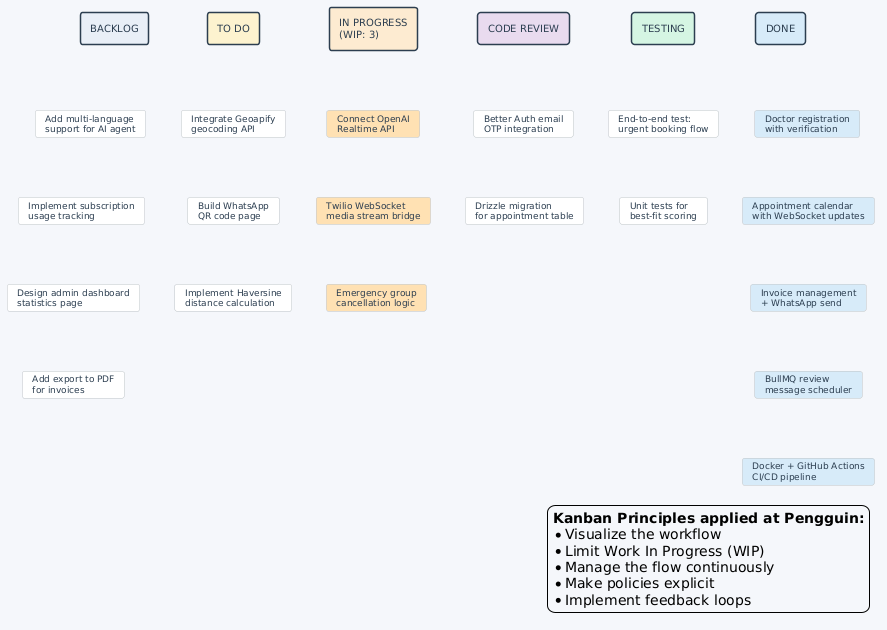
\includegraphics[width=0.8\textwidth]{images/kanban_board_example.png}
    \caption{Example of a Kanban Board Used by the Pengguin Team}
    \label{fig:kanban_board}
\end{figure}

Figure~\ref{fig:kanban_board} shows an example of the Kanban board used by the Pengguin team.

\subsection{Advantages of Kanban for the Riaya Project}
The Kanban method offers several advantages that are particularly relevant to the Riaya project:

\begin{itemize}
    \item \textbf{Flexibility:} Requirements can change at any time, which is essential when integrating AI and real-time communication features. In the Riaya project, the integration of the OpenAI Realtime API and Twilio required constant adjustments based on testing and client feedback \cite{twilio2024, openai2024realtime}. Kanban allowed the team to adapt quickly without being constrained by fixed sprint deadlines. For example, when the AI agent's language model needed to be fine-tuned to better understand Tunisian Arabic, the team was able to reprioritize tasks immediately without waiting for the next sprint.

    \item \textbf{Continuous Delivery:} Features can be delivered as soon as they are ready, allowing the client to provide feedback quickly. This was particularly valuable for the Riaya project, where the client wanted to see incremental progress and test features early. For example, the WhatsApp integration was delivered and tested before the AI voice agent was fully functional, allowing the client to validate the messaging workflow and provide feedback on the message templates.

    \item \textbf{Transparency:} The board gives all team members a clear view of the project status and priorities. This transparency reduces the need for status meetings and helps the team focus on the most important tasks. In the Riaya project, the board was accessible to both the development team and the project manager, ensuring that everyone had a shared understanding of the project's progress. The client also had read-only access to a simplified version of the board, which improved trust and communication.

    \item \textbf{Reduced Bottlenecks:} WIP limits help identify and resolve bottlenecks early, such as the integration of Twilio or OpenAI Realtime API. By limiting the number of tasks in progress, the team could focus on resolving blockers before they escalated. For example, when the Twilio integration encountered issues with WebSocket media streams, the team was able to dedicate resources to resolve the problem without being distracted by other tasks. This early detection prevented the bottleneck from delaying the entire project.

    \item \textbf{Improved Collaboration:} The visual nature of the board encourages communication and teamwork. Team members can see who is working on what and can offer help or advice when needed. In the Riaya project, the board facilitated collaboration between the frontend and backend developers, as well as between the web and voice server teams. When a frontend developer needed a new API endpoint, they could see which backend developer was working on the corresponding card and coordinate directly.

    \item \textbf{Metrics and Continuous Improvement:} Kanban encourages the collection and analysis of metrics such as lead time, cycle time, and throughput. These metrics help the team identify areas for improvement and make data-driven decisions. In the Riaya project, the team used these metrics to optimize their workflow and reduce the time required to deliver features. For example, after analyzing the cycle time of database migration tasks, the team decided to automate more of the migration process, reducing the average cycle time from three days to one day.
\end{itemize}

\subsection{Disadvantages and Limitations of the Method}
Despite its advantages, Kanban also has some limitations that the Pengguin team had to consider:

\begin{itemize}
    \item \textbf{Lack of Timeboxing:} Unlike Scrum, Kanban does not impose fixed iterations (sprints). This can lead to a lack of rhythm and deadlines if not managed carefully. In the Riaya project, the team mitigated this risk by setting internal deadlines and using time-based metrics to track progress. They also established a weekly review meeting to ensure that the project was moving forward at a satisfactory pace.

    \item \textbf{Role Ambiguity:} Kanban does not define specific roles such as Product Owner or Scrum Master. This can cause confusion in larger teams. In the Riaya project, the team was small and cross-functional, so role ambiguity was less of an issue. However, the project manager took on the responsibility of prioritizing tasks and ensuring that the board was up to date. Clear communication and regular stand-up meetings helped prevent misunderstandings.

    \item \textbf{Difficulty in Scaling:} For very large projects, Kanban can become difficult to coordinate without additional frameworks. In the Riaya project, the team was small enough to manage the board effectively. However, if the project were to grow, the team might need to adopt a scaling framework such as Scrum of Scrums or LeSS \cite{larman2016scaling}. This is an important consideration for future phases of the Riaya project.

    \item \textbf{Requires Discipline:} The team must be disciplined to respect WIP limits and keep the board updated. In the Riaya project, the team held daily stand-up meetings to ensure that the board was accurate and that WIP limits were respected. Without this discipline, the board could become outdated and lose its value. The project manager also performed regular audits of the board to ensure that it reflected reality.

    \item \textbf{Lack of Emphasis on Quality:} Kanban does not prescribe specific quality practices such as test-driven development (TDD) or code reviews \cite{beck2002tdd}. In the Riaya project, the team adopted these practices independently to ensure the quality of the code. The ``Code Review'' and ``Testing'' columns on the board helped enforce these practices. Automated tests were run on every pull request, and code reviews were mandatory before merging.
\end{itemize}

\subsection{Comparative Table: Kanban vs Scrum vs Waterfall (V-Model)}
Table~\ref{tab:comparison_methods} compares the three main project management methodologies considered by the Pengguin team.

\begin{table}[H]
    \centering
    \caption{Comparison of Kanban, Scrum, and Waterfall}
    \label{tab:comparison_methods}
    \small
    \begin{tabular}{p{2.5cm}p{3.5cm}p{3.5cm}p{3.5cm}}
        \toprule
        \textbf{Criteria} & \textbf{Kanban} & \textbf{Scrum} & \textbf{Waterfall (V-Model)} \\
        \midrule
        Approach & Continuous flow & Iterative (sprints) & Sequential \\
        Roles & Not defined & Product Owner, Scrum Master, Team & Project Manager \\
        Changes & At any time & Between sprints & Difficult after validation \\
        Delivery & Continuous & At the end of each sprint & At the end of the project \\
        WIP Limits & Yes & Implicit (sprint backlog) & No \\
        Meetings & Daily stand-up (optional) & Sprint planning, daily stand-up, review, retrospective & Milestone reviews \\
        Metrics & Lead time, cycle time, throughput & Velocity, burndown chart & Earned value management \\
        Best suited for & Support, DevOps, evolving projects & Complex products with changing requirements & Projects with fixed requirements \\
        \bottomrule
    \end{tabular}
    \\[0.2cm]
    \small Source: Adapted from Kniberg, H., \& Skarin, M. (2010). \textit{Kanban and Scrum: Making the Most of Both}. InfoQ \cite{kniberg2010kanban}.
\end{table}

\subsection{Justification of the Choice of Kanban by the Pengguin Team}
The Pengguin team chose Kanban for the Riaya project for several reasons.

First, the project involves a high degree of uncertainty and innovation, particularly in the integration of AI voice agents and real-time WebSocket communication. Kanban's flexibility allows the team to adapt quickly to technical challenges and client feedback. When the OpenAI Realtime API was first integrated, its behaviour differed from initial assumptions, and the team needed to adjust the prompt engineering and tool calling strategy. Kanban allowed this without disrupting the overall schedule.

Second, the project is developed by a small, cross-functional team that can benefit from the transparency and self-organization promoted by Kanban. Each developer was responsible for multiple areas (frontend, backend, DevOps), and the board helped them coordinate without the overhead of formal ceremonies.

Third, the continuous delivery model aligns well with the client's desire to see incremental progress and to test features early. The client was able to test the WhatsApp integration, the AI voice agent, and the doctor dashboard at different stages, providing valuable feedback that shaped subsequent iterations.

Fourth, the use of a digital Kanban board facilitates remote collaboration and integration with the CI/CD pipeline. The board was accessible from any device, and the GitHub integration ensured that each pull request was linked to its corresponding card. This provided full traceability from requirements to code and helped the team maintain a clear overview of the project at all times.

Finally, an important factor in the choice of Kanban was the need to handle urgent production issues alongside planned development work. Because Riaya is a live platform that handles real patient calls, the team needed a method that could accommodate unplanned work without disrupting the entire schedule. Kanban's flexible structure allowed the team to insert urgent tasks into the board and to prioritize them without having to wait for the next sprint. This was particularly valuable during the early weeks of production, when unexpected issues required immediate attention.

\begin{figure}[H]
    \centering
    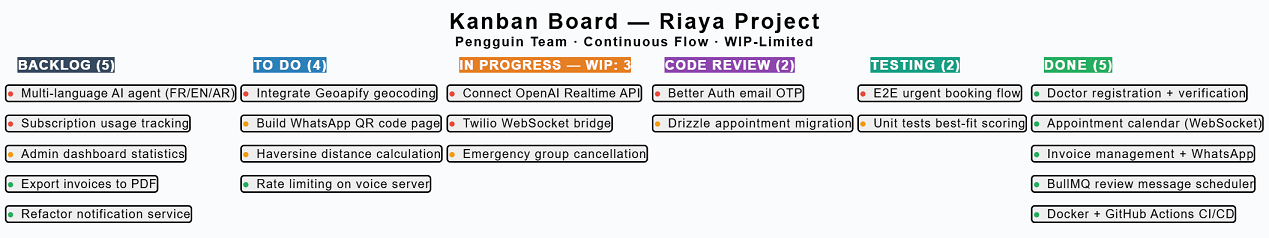
\includegraphics[width=0.8\textwidth]{images/kanban_board_riaya.png}
    \caption{Kanban Board Used in the Riaya Project}
    \label{fig:kanban_riaya}
    \small Source: Pengguin Internal Documentation.
\end{figure}

Figure~\ref{fig:kanban_riaya} shows the Kanban board actually used during the Riaya project.

\section{List and Presentation of Modeling Diagrams}
The modeling of a complex system such as Riaya requires a set of complementary diagrams, each capturing a different view of the system \cite{omg2017uml, fowler2003uml}. The Pengguin team used six main diagrams: the use case diagram, the class/ERD diagram, the sequence diagram, the activity diagram, the deployment diagram, and the BPMN diagram. The following subsections present each of them in detail.

\subsection{Use Case Diagram: Presentation of Actors and Their Interactions}
The use case diagram provides a high-level view of the interactions between the actors (Patient, Doctor, Administrator) and the Riaya system. It shows the main use cases such as ``Book an appointment'', ``Manage patients'', ``Verify doctors'', and ``Monitor live calls''. This diagram is essential for understanding the functional scope of the platform and for communicating with stakeholders who may not be familiar with technical details.

The use case diagram includes three main actors:

\begin{itemize}
    \item \textbf{Patient:} The patient interacts with the system through phone calls and WhatsApp. The main use cases include ``Call Riaya and speak with the booking assistant'', ``Book an appointment'', ``Request urgent booking'', ``Consult or cancel an existing AI booking'', ``Receive doctor messages on WhatsApp'', ``Rate a doctor after a visit'', and ``Be notified if a request expires''. The patient does not need to authenticate because the phone number is used as the unique identifier.
    
    \item \textbf{Doctor:} The doctor interacts with the system through a web dashboard. The main use cases include ``Register and apply for verification'', ``Manage practice profile and availability'', ``Manage patients'', ``Manage appointments'', ``Manage medical documentation'', ``Manage patient billing'', ``Record and transcribe consultations'', ``Use the practice AI assistant'', ``Connect WhatsApp'', and ``Manage Riaya subscription''. Most of these use cases require the doctor to be authenticated and verified.
    
    \item \textbf{Administrator:} The administrator interacts with the system through a dedicated back-office. The main use cases include ``Review and verify doctors'', ``Monitor the AI booking channel'', ``Operate platform configuration'', and ``View platform overview''. The administrator has the highest level of access and can manage all aspects of the platform.
\end{itemize}

The use case diagram also shows the relationships between use cases, such as ``include'' and ``extend''. For example, the ``Book an appointment'' use case includes ``Authenticate'' for the doctor, and the ``Register and apply for verification'' use case includes ``Verify email OTP''. These relationships help clarify the dependencies between use cases and ensure that all necessary steps are accounted for.

\begin{figure}[H]
    \centering
    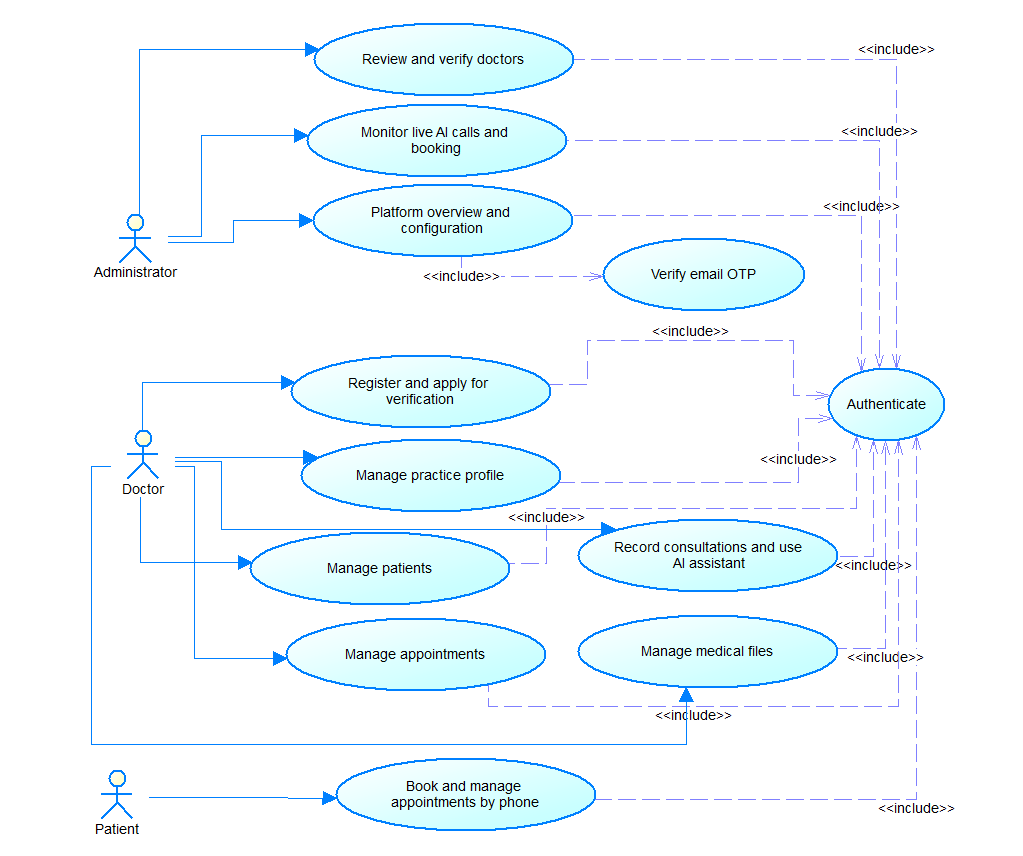
\includegraphics[width=0.8\textwidth]{images/use_case_diagramdsdsd.png}
    \caption{Use Case Diagram of Riaya}
    \label{fig:use_case}
\end{figure}

The use case diagram presented in Figure~\ref{fig:use_case} provides a high-level view of the interactions between the three main actors of the Riaya platform --- the Patient, the Doctor, and the Administrator --- and the system itself. The system boundary is represented by the rectangle labelled ``Riaya'', which encloses all the use cases offered by the platform.

The \textbf{Patient} interacts with the system exclusively through phone calls and WhatsApp, without any account creation. The patient's use cases include: \textit{Call Riaya and speak with the AI assistant}, \textit{Book an appointment (standard or urgent)}, \textit{Consult or cancel pending appointments}, \textit{Receive WhatsApp messages from the doctor}, \textit{Rate a doctor after a visit}, and \textit{Be notified if a request expires}.

The \textbf{Doctor} interacts with the system through a secure web dashboard. The doctor's use cases include: \textit{Register and apply for verification}, \textit{Manage practice profile and availability}, \textit{Manage patients}, \textit{Manage appointments}, \textit{Manage medical files and documents}, \textit{Manage invoices and send via WhatsApp}, \textit{Record consultations and use the AI assistant}, and \textit{Manage subscription and connect WhatsApp}. Most of these use cases require the doctor to be authenticated and verified.

The \textbf{Administrator} uses a dedicated back-office. The administrator's use cases include: \textit{Review and verify doctors}, \textit{Monitor live AI calls and booking}, and \textit{Platform overview and configuration}.

The diagram also shows the \texttt{<<include>>} relationships. For example, the \textit{Register and apply for verification} use case includes \textit{Verify email OTP}, which is a mandatory step. Similarly, all doctor and administrator use cases that require dashboard access include the \textit{Authenticate (sign in)} use case. These relationships clarify the dependencies between use cases and ensure that all necessary steps are accounted for in the functional design of the platform.

Overall, the use case diagram helps to communicate the functional scope of Riaya to both technical and non-technical stakeholders, and it serves as a reference for validating that all user needs are covered by the system.

\subsection{Class Diagram / ERD: Modeling the PostgreSQL Database}
The class diagram, also known as the Entity-Relationship Diagram (ERD), models the database schema of the Riaya platform. It includes entities such as \texttt{doctor\_profile}, \texttt{patient}, \texttt{appointment}, \texttt{invoice}, \texttt{consultation}, \texttt{whatsapp\_session}, and \texttt{subscription}. The ERD shows the relationships between these entities, including cardinalities (one-to-many, many-to-one) and key attributes. This diagram is crucial for designing the PostgreSQL database \cite{postgresql2024} accessed through Drizzle ORM \cite{drizzle2024}.

The main entities and their relationships are as follows:

\begin{itemize}
    \item \textbf{Doctor\_Profile:} Stores the professional information of the doctor, including first name, last name, CIN picture, speciality, Medical Council registration number, Medical Council certificate, cabinet name, TIN, cabinet city, and exact cabinet location (latitude and longitude). A doctor has one profile and can have many appointments, consultations, invoices, and WhatsApp sessions.
    
    \item \textbf{Patient:} Stores the patient's information, including first name, last name, date of birth, gender, address, preferred language, and phone number. A patient can have many appointments and consultations. The phone number is the unique identifier and is used to match the caller when they dial the Riaya number.
    
    \item \textbf{Appointment:} Stores the appointment details, including date and time, status (pending, confirmed, cancelled), reason for the visit, and emergency group ID (for urgent requests). An appointment is linked to one doctor and one patient. The emergency group ID allows multiple urgent appointments to be linked together so that they can be cancelled as a group if needed.
    
    \item \textbf{Invoice:} Stores the invoice details, including amount, status (paid, unpaid), and date. An invoice is linked to one doctor and one patient. Invoices can be sent to the patient via WhatsApp.
    
    \item \textbf{Consultation:} Stores the consultation notes, prescriptions, and medical documents. A consultation is linked to one doctor and one patient. Medical documents are stored in Cloudflare R2 \cite{cloudflare2024r2}, and the consultation record contains a reference to the stored file.
    
    \item \textbf{WhatsApp\_Session:} Stores the WhatsApp session details, including the linked phone number and session status. A WhatsApp session is linked to one doctor. The session is established when the doctor scans a QR code, and it allows the platform to send messages from the doctor's own number.
    
    \item \textbf{Subscription:} Stores the subscription details, including plan type (Free or Pro), start date, end date, and usage limits. A subscription is linked to one doctor. Usage limits are tracked to enforce the Free plan restrictions.
\end{itemize}

The ERD also includes join tables and foreign keys that enforce referential integrity. For example, the \texttt{appointment} table has foreign keys pointing to both the \texttt{doctor\_profile} and \texttt{patient} tables, ensuring that every appointment is associated with a valid doctor and patient. The use of Drizzle ORM allows these relationships to be defined in TypeScript, providing type safety and reducing the risk of runtime errors.

\begin{figure}[H]
    \centering
    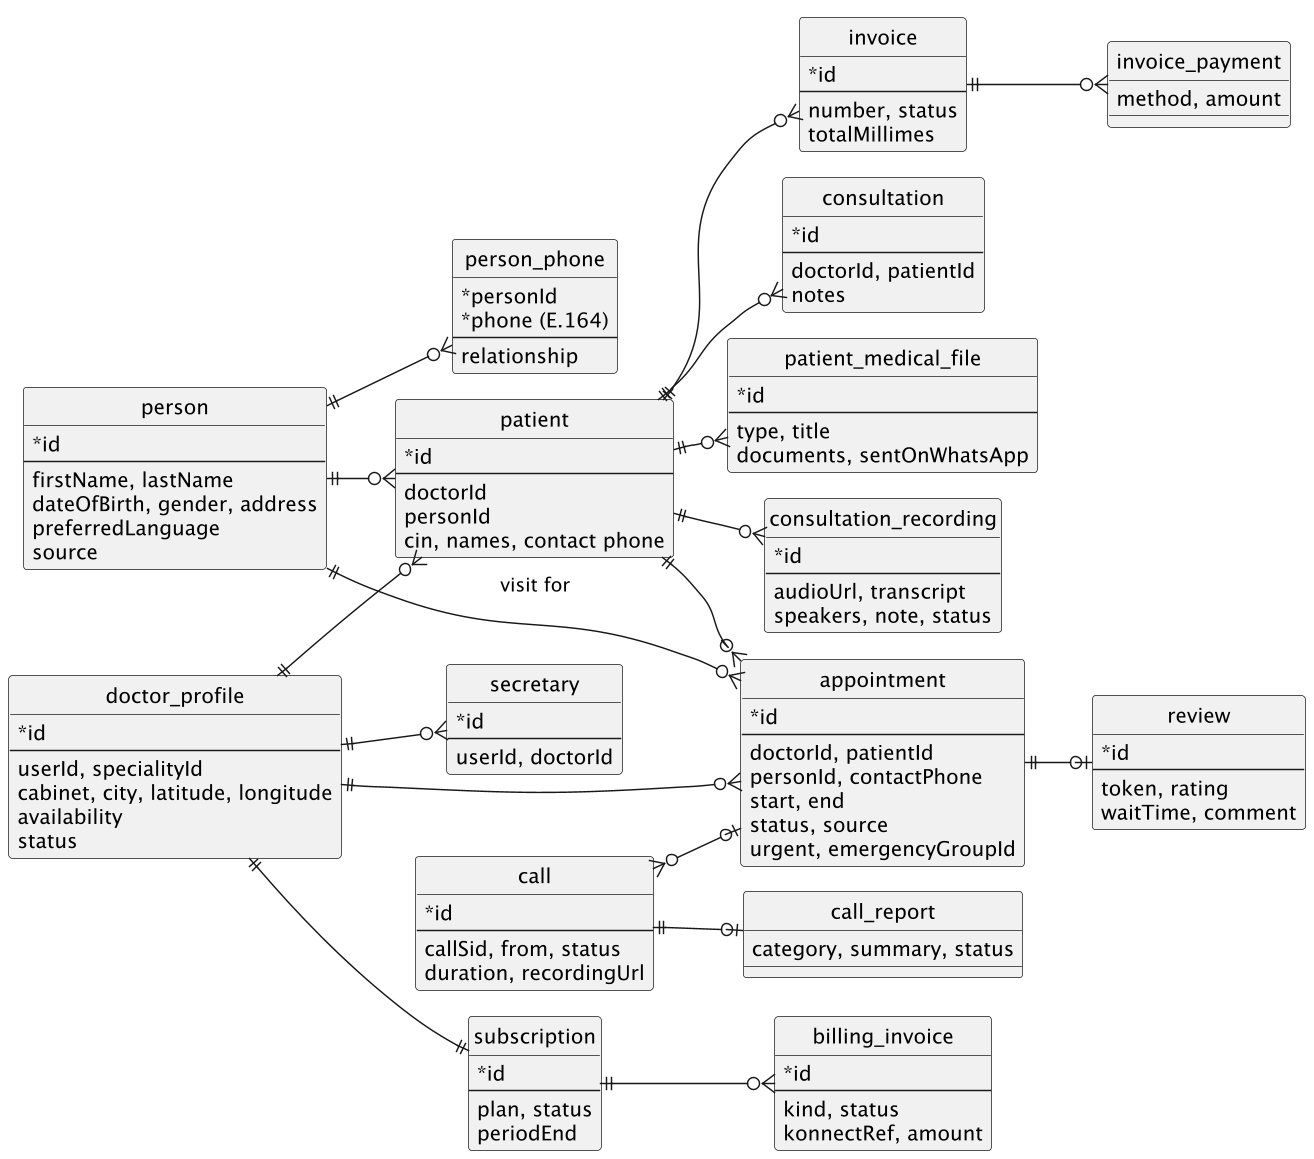
\includegraphics[width=0.9\textwidth]{images/erd_diagram.png}
    \caption{Entity-Relationship Diagram of the Riaya Database}
    \label{fig:erd}
\end{figure}

Figure~\ref{fig:erd} presents the complete ERD of the Riaya database, showing all entities and their relationships.

\subsection{Sequence Diagram: Twilio Call Flow \texorpdfstring{$\rightarrow$}{→} WebSocket \texorpdfstring{$\rightarrow$}{→} OpenAI \texorpdfstring{$\rightarrow$}{→} Database}
The sequence diagram illustrates the real-time flow of a patient's phone call. It shows the interactions between Twilio, the Express.js voice server, the OpenAI Realtime API (via Microsoft Azure), and the PostgreSQL database. The diagram details how the call is received, how the WebSocket media stream is established, how the AI processes speech and makes tool calls to the database, and how the live transcript is sent to the admin dashboard.

The sequence of events is as follows:

\begin{enumerate}
    \item The patient dials the Riaya phone number.
    \item Twilio receives the call and sends a webhook to the Express.js voice server.
    \item The Express.js server looks up or creates the caller in the PostgreSQL database. If the caller is new, a patient record is created with the phone number as the unique identifier.
    \item The server responds with TwiML that opens a WebSocket media stream from Twilio to the server.
    \item The server establishes a WebSocket connection with the OpenAI Realtime API (via Microsoft Azure).
    \item The patient's speech is streamed to the AI, and the AI's voice is streamed back through Twilio onto the phone.
    \item The AI makes tool calls to the database to search for doctors, check availability, and create appointments. These tool calls are executed by the Express.js server, which queries the database and returns the results to the AI.
    \item The live transcript is sent to the admin dashboard via WebSocket, allowing administrators to monitor the call in real time.
    \item When the call ends, the Twilio stream closes, and the session is marked as completed in the database.
\end{enumerate}

This sequence diagram is particularly important because it captures the complexity of the real-time interaction between multiple systems. It helps developers understand the flow of data and the responsibilities of each component, and it serves as a reference for debugging and optimization.

\begin{figure}[H]
    \centering
    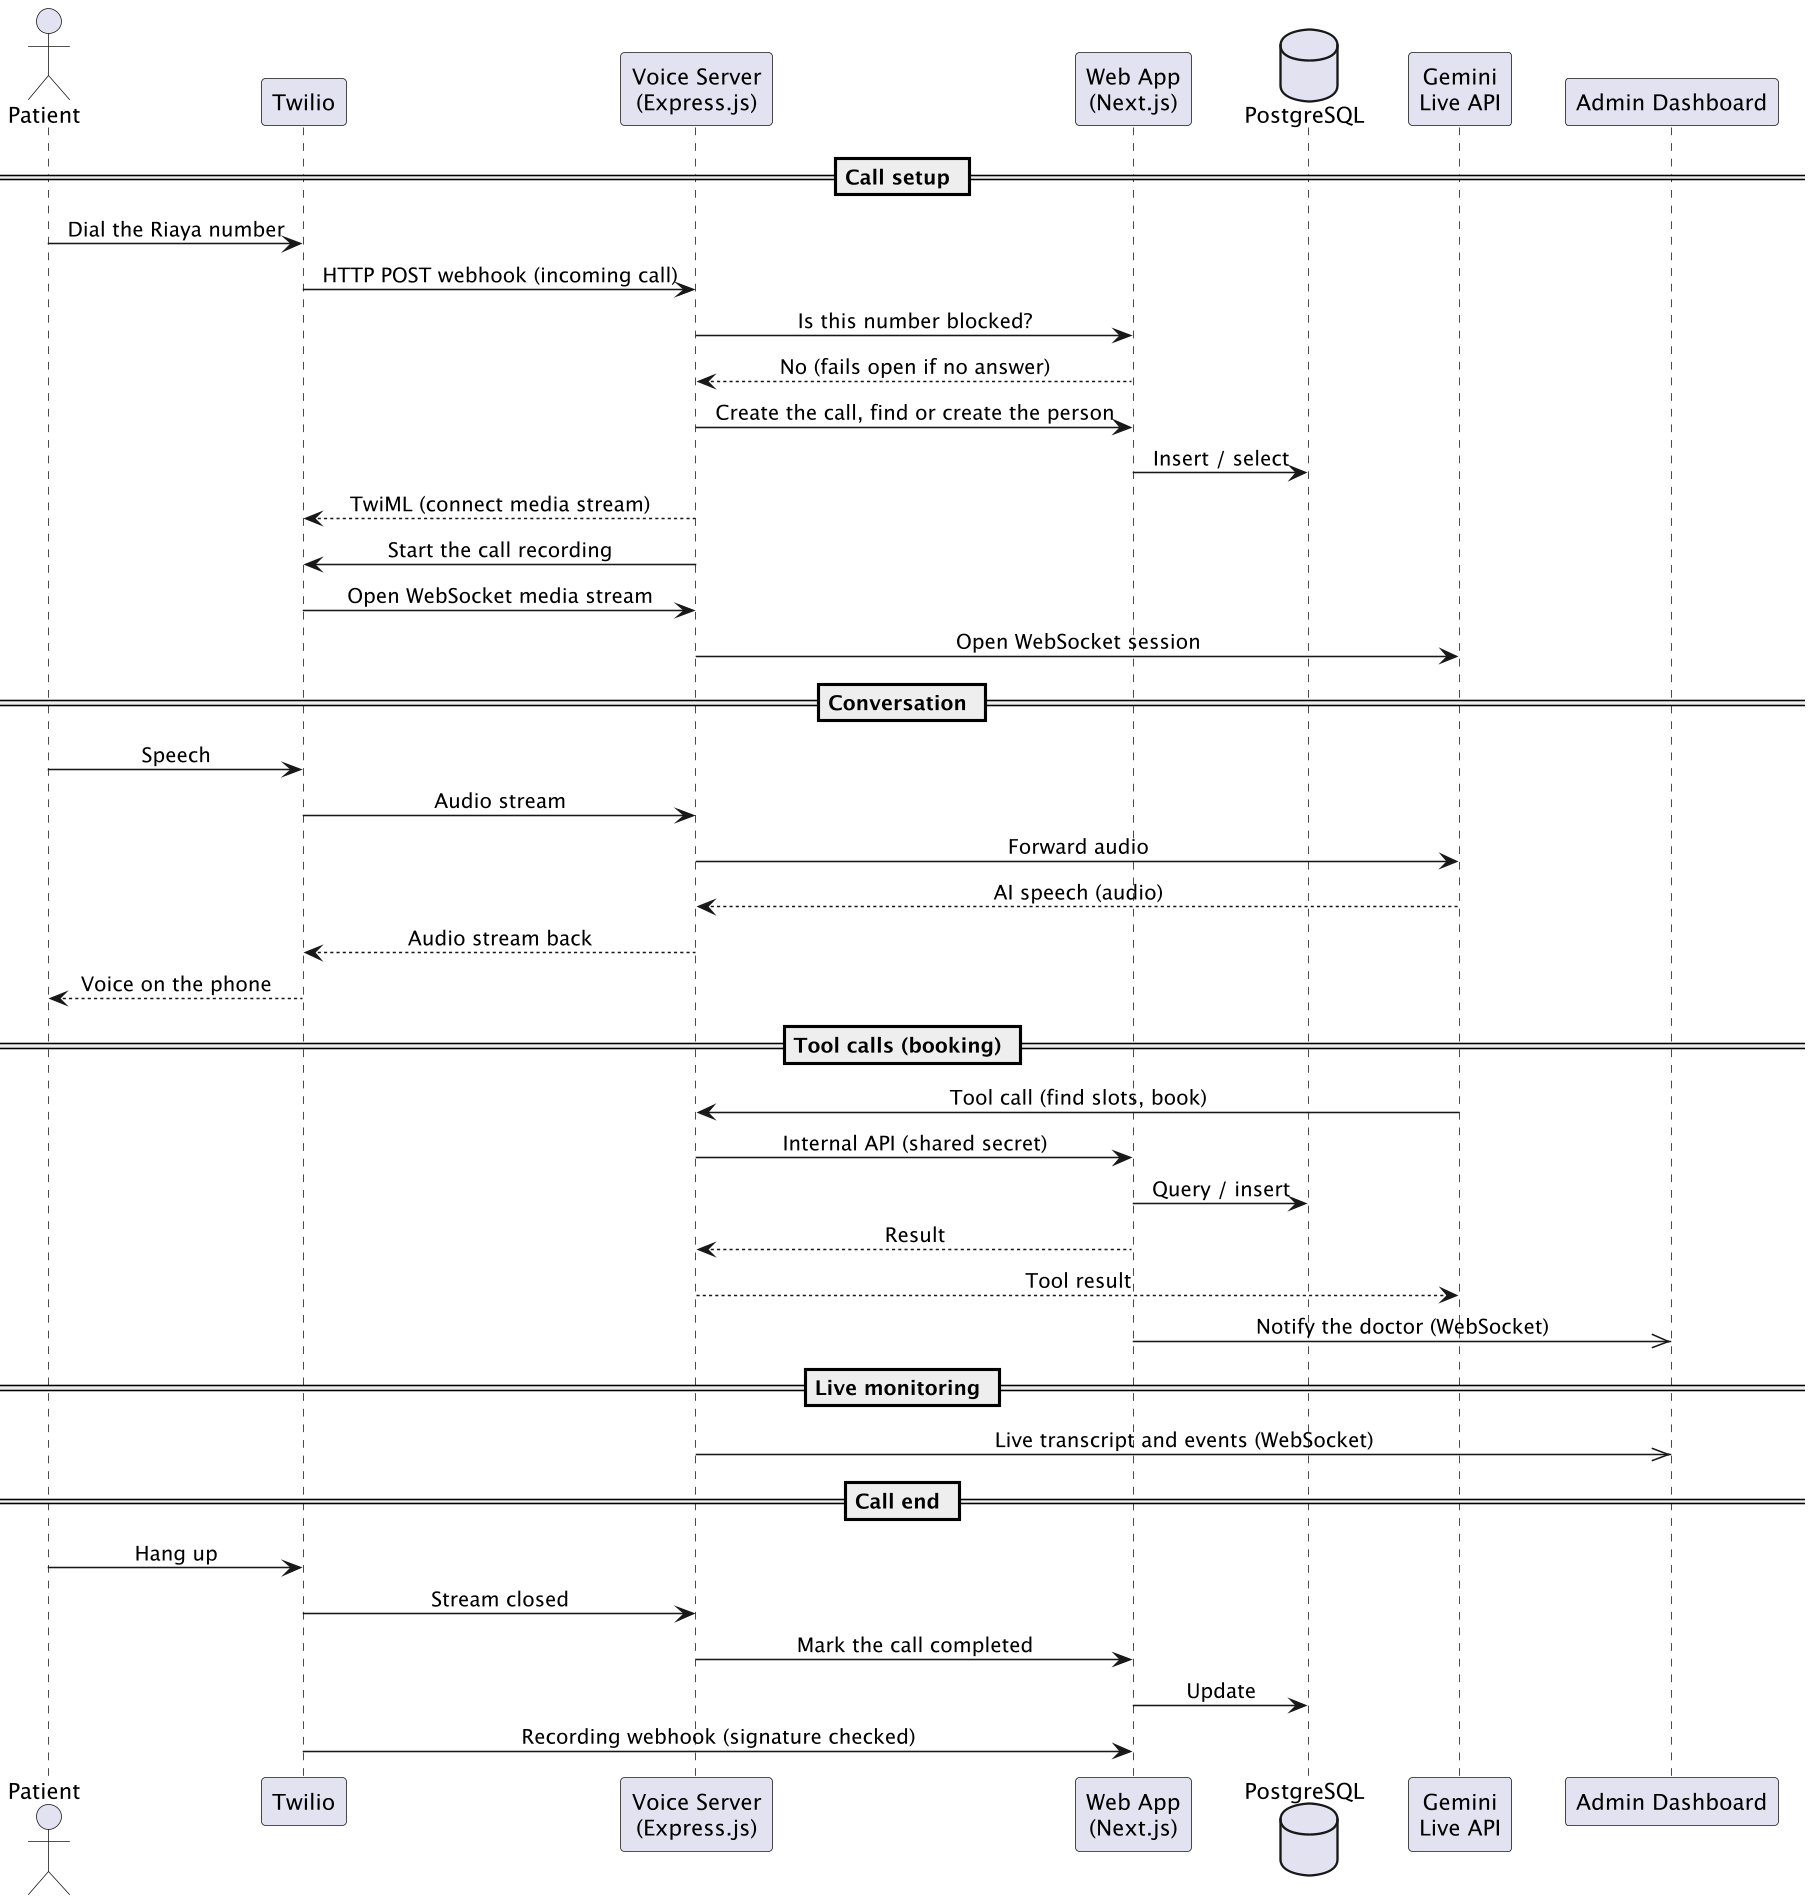
\includegraphics[width=0.9\textwidth]{images/sequence_call_flow.png}
    \caption{Sequence Diagram of the AI Call Flow}
    \label{fig:sequence_call}
\end{figure}

The sequence diagram presented in Figure~\ref{fig:sequence_call} illustrates the real-time flow of a patient's phone call through the Riaya platform. It captures the interactions between six main components: the Patient, Twilio (telephony provider), the Express.js Voice Server, the OpenAI Realtime API (accessed via Microsoft Azure), the PostgreSQL database (managed through Drizzle ORM), and the Admin Dashboard. This diagram is particularly important because it highlights the complexity of the real-time interaction between multiple systems and clarifies the responsibilities of each component.

The sequence begins when the \textbf{Patient} dials the Riaya phone number. \textbf{Twilio} receives the call and sends an HTTP POST webhook to the \textbf{Express.js Voice Server}. The server then looks up or creates the caller in the \textbf{PostgreSQL} database using the phone number as the unique identifier. If the caller is new, a patient record is created. The server responds to Twilio with a TwiML (Twilio Markup Language) instruction that opens a bidirectional WebSocket media stream from Twilio to the server.

Once the WebSocket stream is established, the \textbf{Voice Server} connects to the \textbf{OpenAI Realtime API} via a WebSocket session. From this point, the patient's speech is streamed as audio from Twilio to the Voice Server, which forwards it to the AI. The AI processes the speech and returns synthesized voice audio, which is streamed back through the Voice Server and Twilio to the patient's phone, enabling a natural, low-latency conversation.

During the conversation, the AI can make \textbf{tool calls} back into the Riaya system. These tool calls allow the AI to search for doctors, check availability, and create appointments. The Voice Server executes these tool calls by querying or updating the \textbf{PostgreSQL} database, and returns the results to the AI. This interaction is essential for the booking process.

Simultaneously, the Voice Server pushes the live conversation transcript to the \textbf{Admin Dashboard} via WebSocket, allowing administrators to monitor ongoing calls in real time for operational and debugging purposes.

When the call ends, the patient hangs up, Twilio closes the media stream, and the Voice Server marks the session as completed in the database. Finally, the server may notify the doctor about a pending appointment via WebSocket, triggering the next step in the booking workflow.

In summary, this sequence diagram provides a clear reference for developers to understand the data flow between the telephony, AI, database, and monitoring components. It also serves as a valuable tool for debugging and optimizing the real-time performance of the platform, ensuring that the voice interaction remains fluid and responsive.

\subsection{Activity Diagram: Urgent Booking Process and OTP Authentication}
The activity diagram models the dynamic aspects of two critical processes: the urgent booking process and the OTP authentication. These diagrams are essential for understanding the workflow of the system and for identifying potential issues early in the design phase.

\begin{itemize}
    \item \textbf{Urgent Booking Process:} The AI detects an urgent situation, confirms with the patient, runs an ASAP best-fit search, creates up to three urgent pending appointments linked by an emergency group ID, and waits for the first doctor to accept. If no doctor accepts within 10 minutes, the group is cancelled and the patient is notified. The activity diagram shows the flow of activities, decision points, and parallel processes. It highlights the importance of handling urgency efficiently and ensuring that the patient is not left without a solution.
    
    \item \textbf{OTP Authentication:} The doctor registers with an email, receives an OTP, enters it, and completes the registration. The OTP is verified against the Drizzle verification table. The activity diagram shows the flow of activities, decision points (e.g., OTP valid or invalid), and the final state (account created or registration failed). This process is critical for ensuring that only legitimate doctors can access the platform.
\end{itemize}

These activity diagrams provide a clear and detailed view of the workflows, making it easier to identify potential issues and to communicate the design to stakeholders.

\begin{figure}[H]
    \centering
    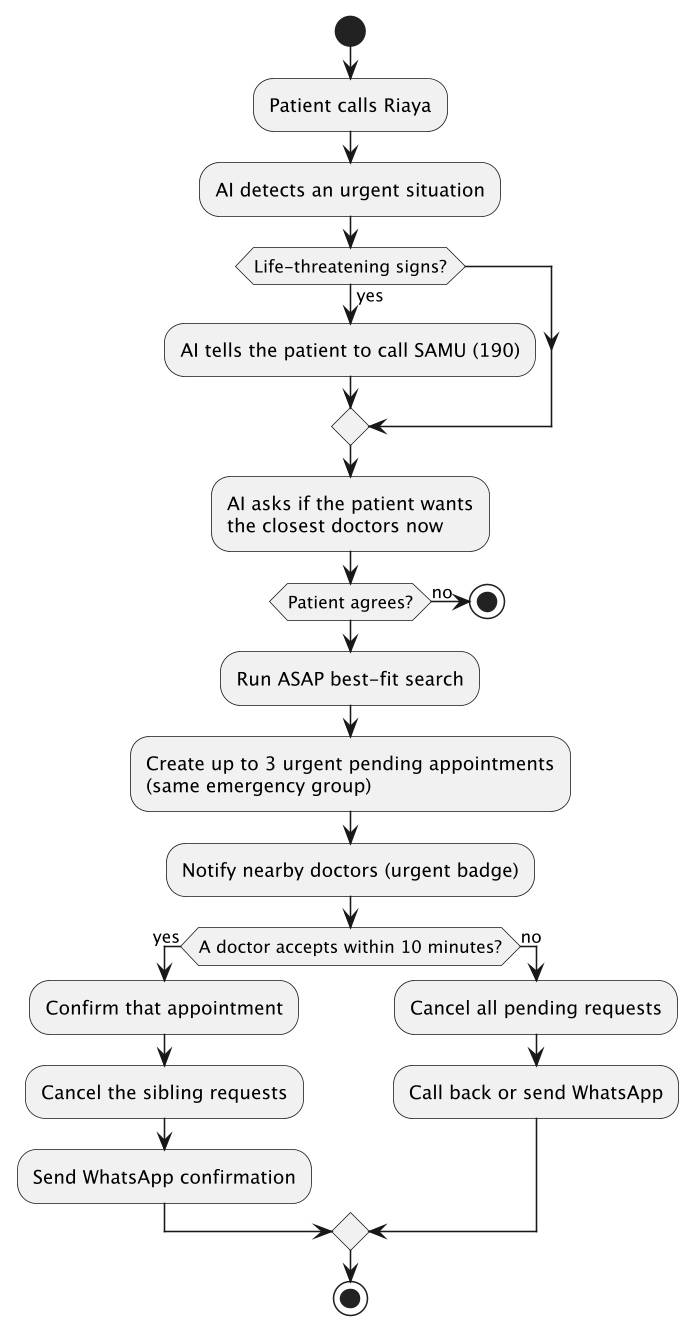
\includegraphics[width=0.8\textwidth]{images/activity_urgent_booking.png}
    \caption{Activity Diagram of the Urgent Booking Process}
    \label{fig:activity_urgent}
\end{figure}

The activity diagram presented in Figure~\ref{fig:activity_urgent} illustrates the workflow of the urgent booking process on the Riaya platform. The flow begins when the patient calls Riaya. The AI assistant detects the urgency of the situation and confirms it with the patient. An ASAP best-fit search is immediately launched, followed by the creation of up to three urgent pending appointments, linked together by an emergency group identifier. Nearby doctors are then notified. A decision point then occurs: if the first doctor accepts within 10 minutes, the appointment is confirmed, the other requests in the group are automatically cancelled, and a confirmation is sent to the patient via WhatsApp. Otherwise, all pending requests are automatically cancelled, and the patient is called back or notified via WhatsApp. The process then ends. This diagram highlights the parallel management of urgent requests and the timeout mechanism that guarantees that no patient is left without a solution.

\begin{figure}[H]
    \centering
    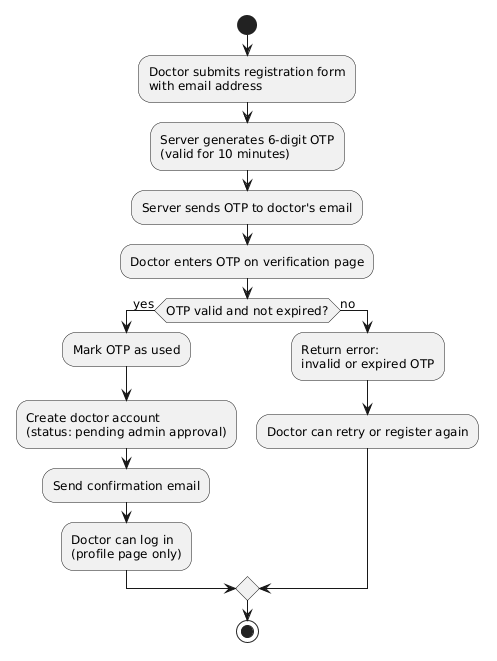
\includegraphics[width=0.8\textwidth]{images/activity_otp_auth.png}
    \caption{Activity Diagram of OTP Authentication}
    \label{fig:activity_otp}
    \small Source: Author's own work based on Riaya internal documentation.
\end{figure}

The activity diagram shown in Figure~\ref{fig:activity_otp} illustrates the OTP-based authentication process used by doctors when registering on the Riaya platform. The process starts when the doctor submits the registration form with an email address. The server then generates a six-digit one-time password (OTP), valid for ten minutes, and sends it to the doctor's email address. The doctor enters the OTP on the verification page. A decision point follows: if the OTP is valid and has not expired, it is marked as used, a doctor account is created with a status of \textit{pending administrator approval}, a confirmation email is sent, and the doctor can log in but can only access the profile page. If the OTP is invalid or expired, an error is returned, and the doctor can either retry entering the OTP or restart the registration process. The process ends after either outcome. This diagram highlights the security measures implemented during registration, including the single-use OTP and the temporary restriction of access until administrator approval.

\subsection{Deployment Diagram: Docker, Nginx, Ubuntu VPS Architecture}
The deployment diagram shows the physical and logical infrastructure of the Riaya platform \cite{docker2024}. It includes:

\begin{itemize}
    \item \textbf{Two repositories:} Web app (Next.js) and Voice server (Express.js). Each repository has its own GitHub Actions CI/CD workflow.
    \item \textbf{GitHub Actions:} CI/CD pipelines that build Docker images, publish them to GHCR, and deploy to a self-hosted Ubuntu VPS.
    \item \textbf{Nginx:} Reverse proxy handling TLS and routing.
    \item \textbf{Docker containers:} PostgreSQL, Redis, web app, and voice server running on a shared Docker network.
    \item \textbf{External services:} Twilio, OpenAI Realtime API (Azure), Cloudflare R2, Konnect.network, WhatsApp Baileys, Geoapify.
\end{itemize}

The deployment diagram also shows the network connections between the different components, including the WebSocket connections between Twilio and the voice server, and between the voice server and the OpenAI Realtime API. It is an essential tool for understanding how the platform is deployed and for planning maintenance and scaling operations.

\begin{figure}[H]
    \centering
    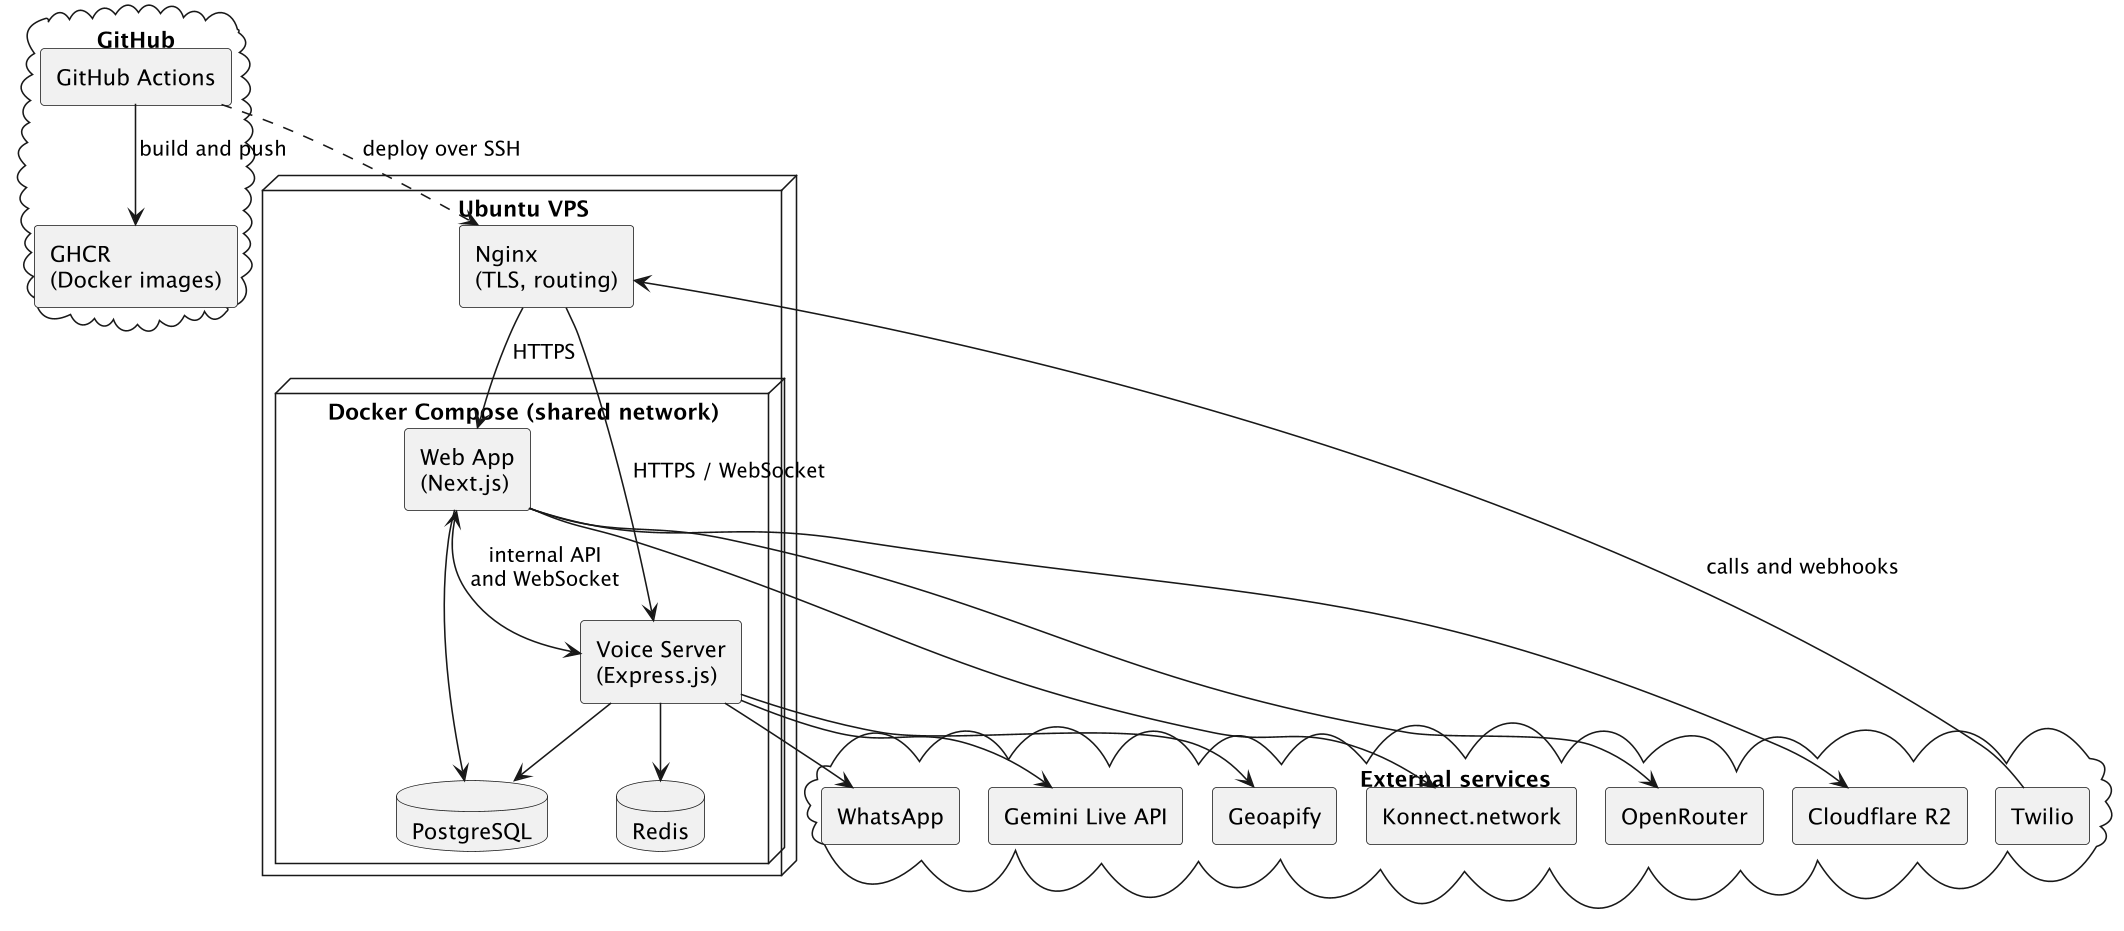
\includegraphics[width=0.9\textwidth]{images/deployment_diagram.png}
    \caption{Deployment Diagram of the Riaya Platform}
    \label{fig:deployment}
\end{figure}

The deployment diagram shown in Figure~\ref{fig:deployment} presents a simplified view of the Riaya platform architecture. The entire system is hosted on an Ubuntu VPS, which runs Nginx as a reverse proxy. Nginx routes HTTP traffic to the Web App (Next.js) and WebSocket connections to the Voice Server (Express.js). Both the Web App and the Voice Server communicate with a PostgreSQL database. The Voice Server also interacts with two external services: it receives incoming phone calls from Twilio and establishes a WebSocket session with the OpenAI Realtime API, which is hosted on Microsoft Azure. This minimal diagram highlights only the core components and their primary connections, omitting secondary services such as Redis, Cloudflare R2, WhatsApp, and payment gateways for clarity.

\subsection{BPMN: Global Business Process}
The BPMN (Business Process Model and Notation) diagram provides a standardized graphical representation of the entire business process of Riaya \cite{omg2011bpmn}. It covers the standard booking flow, the urgent booking flow, and the timeout handling. It includes pools for the patient, the AI system, the doctor, and the administrator, and shows the message flows and sequence flows between them.

The BPMN diagram includes the following main elements:

\begin{itemize}
    \item \textbf{Pools:} Patient, AI System, Doctor, Administrator.
    \item \textbf{Lanes:} Within the AI System pool, lanes for ``Call Handling'', ``Best-fit Search'', ``Appointment Management'', and ``Notification''.
    \item \textbf{Start Events:} Patient calls Riaya, Doctor registers, Administrator logs in.
    \item \textbf{Intermediate Events:} Appointment created, Doctor accepts, Doctor declines, Timeout.
    \item \textbf{End Events:} Appointment confirmed, Appointment cancelled, Registration approved, Registration rejected.
    \item \textbf{Sequence Flows:} The order of activities within each pool.
    \item \textbf{Message Flows:} The communication between pools (e.g., patient calls AI, AI notifies doctor, doctor accepts appointment, AI sends WhatsApp confirmation to patient).
    \item \textbf{Gateways:} Decision points such as ``Is the situation urgent?'' and ``Did the doctor accept within 10 minutes?''.
\end{itemize}

The BPMN diagram is a valuable communication tool that helps both technical and non-technical stakeholders understand the end-to-end process. It also serves as a reference for identifying opportunities for improvement and for ensuring that all scenarios are properly handled.

\begin{figure}[H]
    \centering
    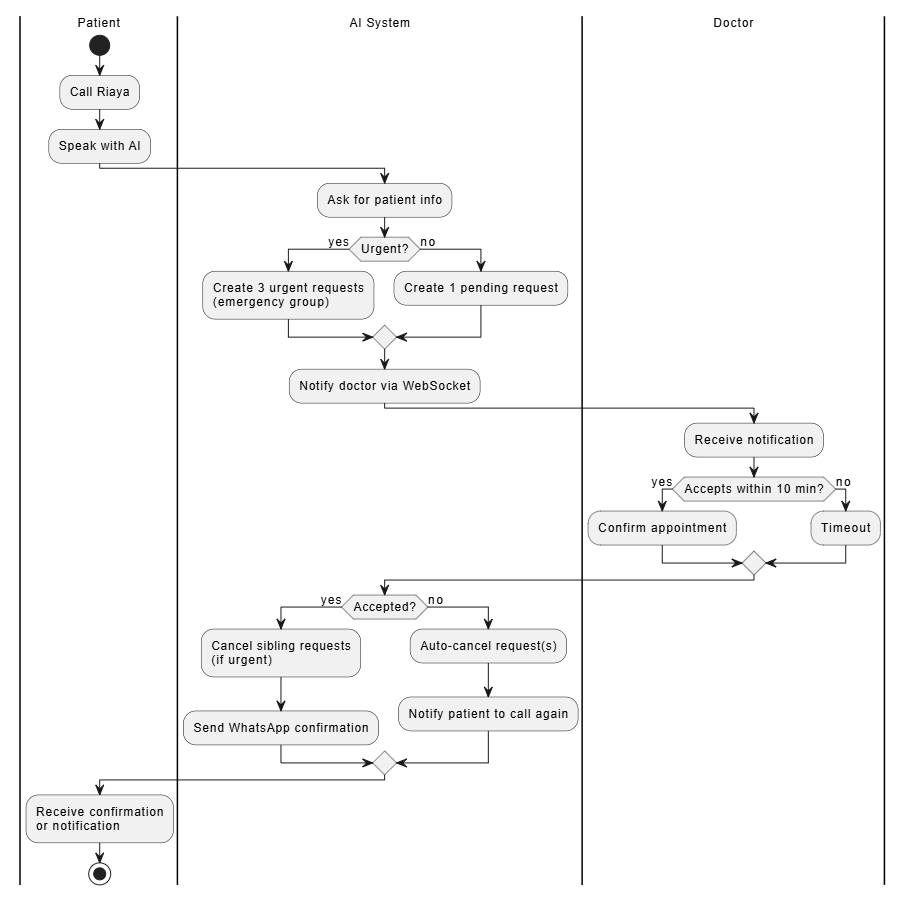
\includegraphics[width=0.9\textwidth]{images/global_bpmn.png}
    \caption{Global BPMN Diagram of the Riaya Project}
    \label{fig:bpmn_global_ch2}
\end{figure}

Figure~\ref{fig:bpmn_global_ch2} presents the global BPMN diagram of the Riaya project, covering all three flows (standard, urgent, and timeout).

\section{Conclusion}
This chapter has presented the Kanban methodology, including its principles, advantages, disadvantages, and a comparative analysis with Scrum and Waterfall. It justified the choice of Kanban for the Riaya project. It also listed and described the main modeling diagrams used in the design of the platform: use case, class/ERD, sequence, activity, deployment, and BPMN. These diagrams provide a solid foundation for understanding both the functional and technical aspects of Riaya. The next chapter will focus on the technical architecture and implementation details.
        \clearpage
        
        \chapter{Technical Architecture, Implementation, and Deployment}

\section{Introduction}
This chapter covers the technical architecture of Riaya, the implementation choices of the Pengguin team, and the deployment strategy that put the product into production. It starts with an overview of the system architecture and the decision to split the project into two repositories, the web application and the voice server. It then goes through the technology stack component by component: frontend, backend, database, voice server, third-party integrations, background jobs, and CI/CD infrastructure. A section of screenshots shows the main features of the platform. The chapter ends with security, confidentiality, and access management, and with the technical challenges the team met and how it solved them.

\section{Global System Architecture}

\subsection{Architectural Principles}
Three architectural principles guided the technical decisions behind Riaya: \textit{separation of concerns}, \textit{event-driven communication}, and \textit{containerized deployment} \cite{fowler2002patterns}. They follow common cloud-native practice and keep the platform maintainable, scalable, and resilient as it grows.

Separation of concerns led to splitting Riaya into two independent repositories. Event-driven communication shows in the heavy use of WebSockets for real-time notifications between the web application and the voice server \cite{fette2011websocket}. Containerized deployment means every component runs in an isolated, reproducible environment managed by Docker \cite{docker2024}.

\subsection{Separation into Two Repositories (Web App and Voice Server)}
One of the team's first architectural decisions was to split Riaya into two repositories:

\begin{itemize}
    \item \textbf{Web App Repository:} Built with Next.js \cite{nextjs2024}, this repository contains the frontend and backend of the doctor and administrator dashboards. It manages authentication, patient records, appointments, invoices, medical documentation, subscriptions, and the WhatsApp configuration page. It communicates with the PostgreSQL database \cite{postgresql2024} through Drizzle ORM \cite{drizzle2024}.
    
    \item \textbf{Voice Server Repository:} Built with Express.js \cite{express2024}, this repository is dedicated to real-time communication. It handles incoming Twilio \cite{twilio2024} calls, WebSocket media streams, the OpenAI Realtime API \cite{openai2024realtime} integration (via Microsoft Azure \cite{azure2024openai}), WhatsApp integration using WhatsApp Baileys \cite{baileys2024}, and background jobs managed by BullMQ \cite{bullmq2024} and Redis \cite{redis2024}.
\end{itemize}

The split has four advantages. The two applications scale independently, which matters because the voice server streams real-time audio and needs very different resources from the web application. Failures stay isolated: a problem in the voice server does not take down the doctor dashboard, and the reverse is also true. The team can deploy one repository without redeploying the other, which speeds up delivery. And each application has a smaller attack surface and access to fewer sensitive credentials.

\begin{figure}[H]
    \centering
    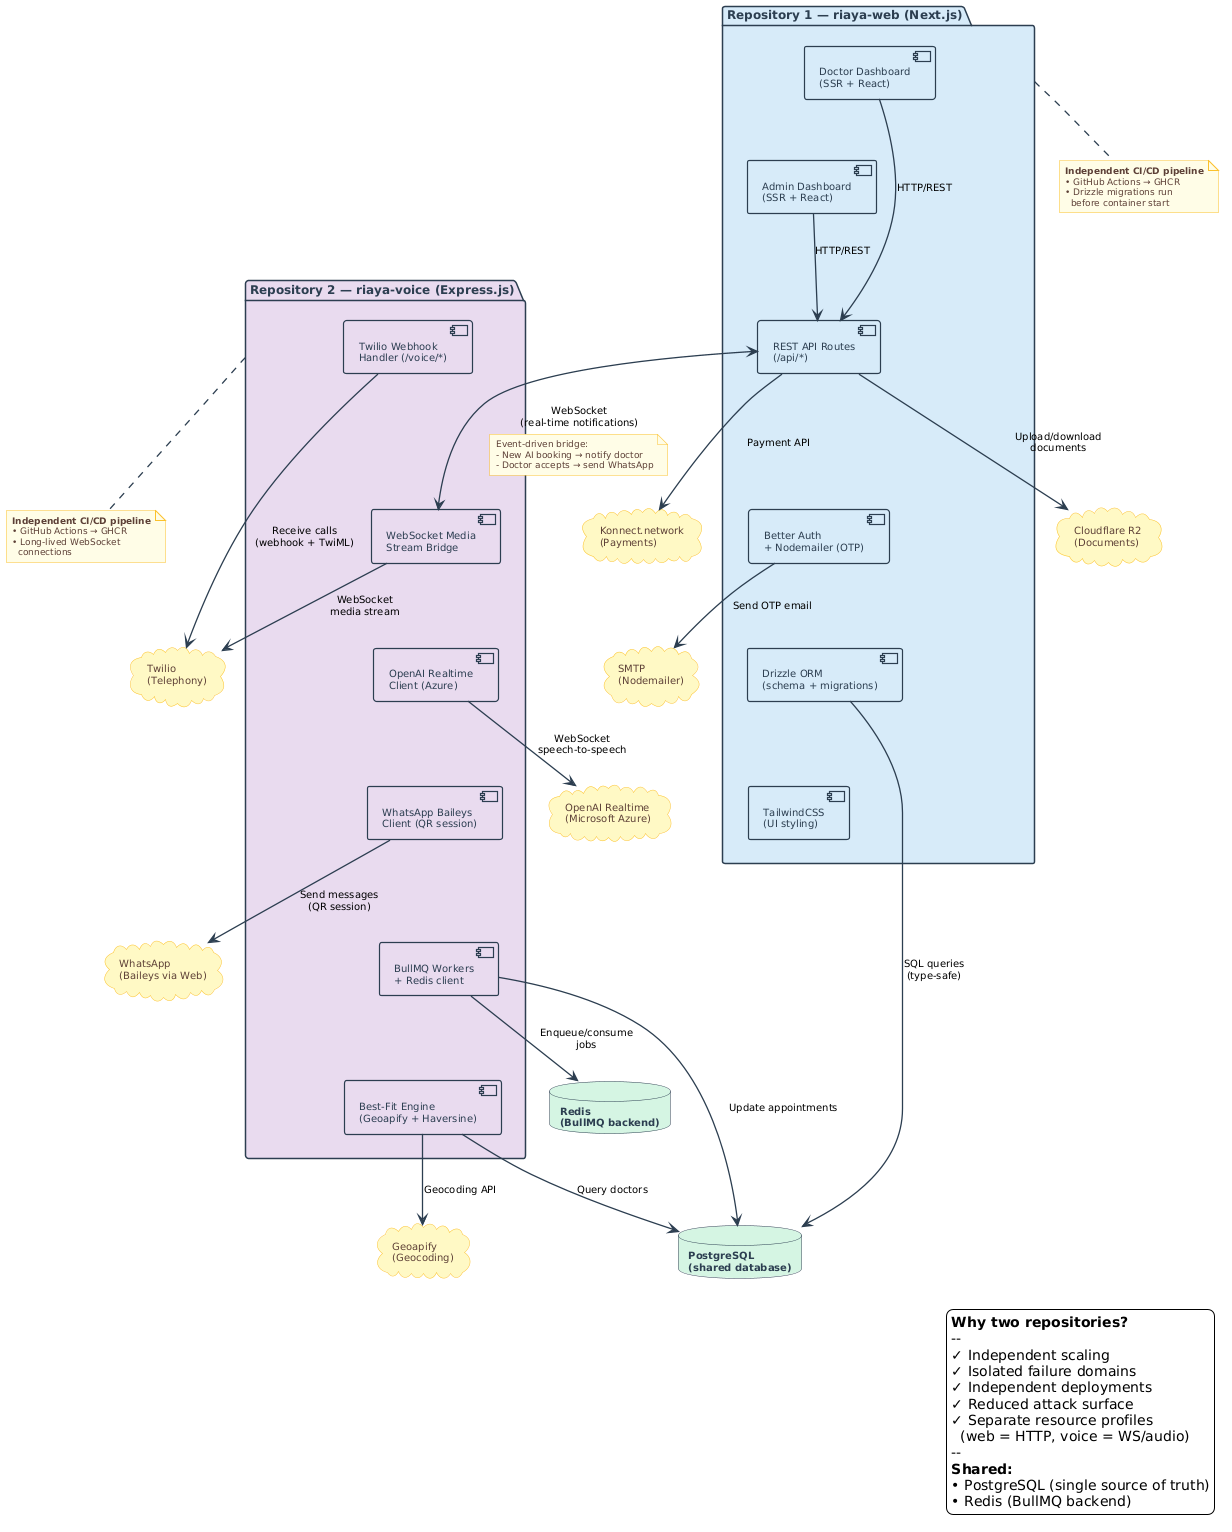
\includegraphics[width=0.85\textwidth,height=0.4\textheight,keepaspectratio]{images/two_repositories_architecture.png}
    \caption{Separation of the Riaya Platform into Two Repositories}
    \label{fig:two_repos}
\end{figure}

Figure~\ref{fig:two_repos} shows the two repositories, each with its own responsibilities and CI/CD pipeline.

\subsection{Technical Architecture Schema (Microservices, Event-Driven)}
Riaya is not a full microservices architecture \cite{newman2015microservices}, but it is service-oriented and event-driven. It is made of loosely coupled components that communicate through well-defined interfaces:

\begin{itemize}
    \item \textbf{Web Application:} Handles HTTP requests, renders the dashboard, and exposes REST endpoints for the doctor and administrator interfaces. It communicates with the database through Drizzle ORM.
    
    \item \textbf{Voice Server:} Handles Twilio webhooks, establishes WebSocket connections, and bridges the audio stream between Twilio and OpenAI Realtime API.
    
    \item \textbf{Database:} A PostgreSQL instance shared by both applications. It stores all persistent data, including doctor profiles, patients, appointments, invoices, consultations, subscriptions, and call logs.
    
    \item \textbf{Redis and BullMQ:} Used for background jobs and scheduled tasks, such as sending review requests two hours after an appointment, generating recurring invoices, and handling timeouts.
    
    \item \textbf{External Services:} Twilio (telephony), OpenAI Realtime API via Microsoft Azure (AI voice agent), Cloudflare R2 \cite{cloudflare2024r2} (file storage), Konnect.network \cite{konnect2024} (payments), WhatsApp Baileys (messaging), and Geoapify \cite{geoapify2024} (geocoding).
\end{itemize}

WebSockets carry the real-time notifications. When the voice server creates a new AI booking, it notifies the web application, which pushes the notification to the doctor's dashboard over a WebSocket. When a doctor accepts or declines an appointment, the web application notifies the voice server, which sends the patient a WhatsApp confirmation.

\begin{figure}[H]
    \centering
    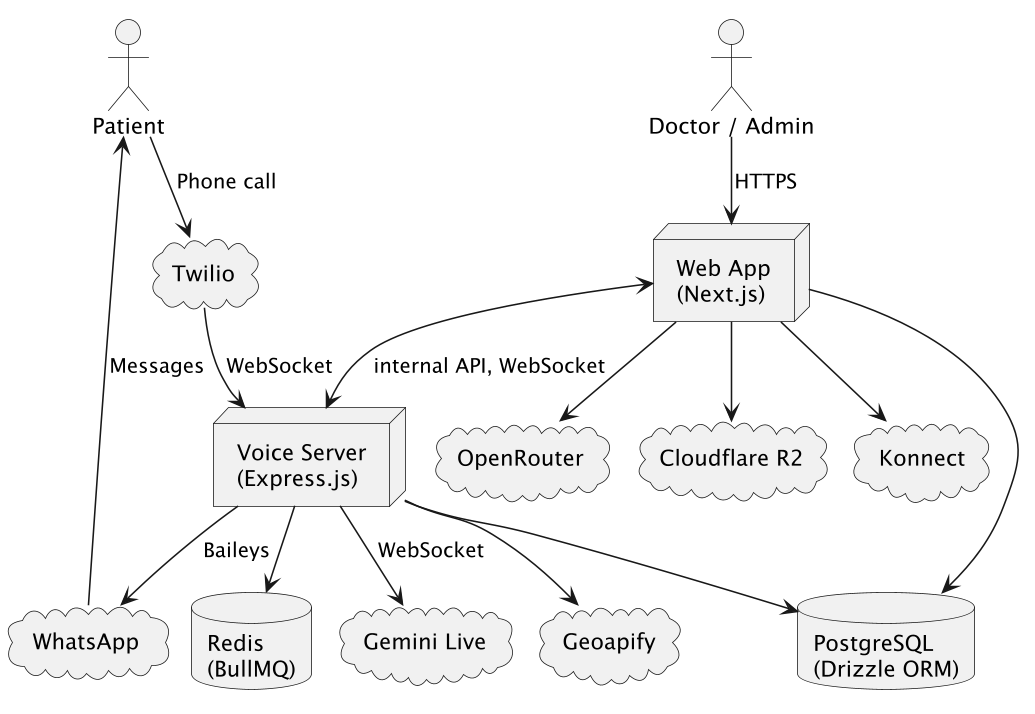
\includegraphics[width=0.85\textwidth,height=0.45\textheight,keepaspectratio]{images/global_architecture_schema.png}
    \caption{Global Technical Architecture of the Riaya Platform}
    \label{fig:global_arch}
\end{figure}

Figure~\ref{fig:global_arch} shows the global technical architecture of Riaya, with all components and their interactions.

\section{Technology Stack and Component Description}
This section goes through the technology stack of Riaya component by component and explains each choice in terms of performance, maintainability, and fit with the project requirements.

\subsection{Frontend and Backend Web: Next.js, TailwindCSS, Better Auth}
The web application is built with \textbf{Next.js} \cite{nextjs2024}, a React framework that supports server-side rendering (SSR), static site generation (SSG), and API routes. The team chose it for its performance, its built-in routing, and because a single codebase can hold both the frontend and the backend. The App Router was preferred over the Pages Router: nested layouts, streaming, and server actions made the complex dashboard pages simpler to build.

Styling uses \textbf{TailwindCSS} \cite{tailwind2024}, a utility-first CSS framework for building responsive interfaces quickly. The team chose it for its flexibility, its small bundle size after tree-shaking, and the consistent design system it enforces across the application.

\textbf{Better Auth} \cite{betterauth2024} handles authentication, with support for email and password, OTP, and session management. When a doctor registers, Riaya emails a one-time password (OTP) using \textbf{Nodemailer}. The OTP is stored in the Drizzle verification table, and the doctor must enter it to complete registration. This mechanism follows the NIST SP 800-63B recommendations on out-of-band authenticators \cite{nist2017sp80063b}.

\begin{figure}[H]
    \centering
    \begin{subfigure}[b]{0.22\textwidth}
        \centering
        
\includegraphics[width=\textwidth,height=2.2cm,keepaspectratio]{images/nextjs.png}
        \caption{Next.js}
        \label{fig:logo_nextjs}
    \end{subfigure}
    \hfill
    \begin{subfigure}[b]{0.22\textwidth}
        \centering
        
\includegraphics[width=\textwidth,height=2.2cm,keepaspectratio]{images/tailwindcss.png}
        \caption{TailwindCSS}
        \label{fig:logo_tailwind}
    \end{subfigure}
    \hfill
    \begin{subfigure}[b]{0.22\textwidth}
        \centering
        
\includegraphics[width=\textwidth,height=2.2cm,keepaspectratio]{images/better-auth.png}
        \caption{Better Auth}
        \label{fig:logo_betterauth}
    \end{subfigure}
    \hfill
    \begin{subfigure}[b]{0.22\textwidth}
        \centering
        
\includegraphics[width=\textwidth,height=2.2cm,keepaspectratio]{images/nodemailer.png}
        \caption{Nodemailer}
        \label{fig:logo_nodemailer}
    \end{subfigure}
    \caption{Logos of the frontend and backend web technologies}
    \label{fig:logos_frontend}
\end{figure}

Figure~\ref{fig:logos_frontend} shows the logos of the web stack technologies.

\subsection{Database: PostgreSQL and Drizzle ORM}
The main database is \textbf{PostgreSQL} \cite{postgresql2024}, an open-source relational database known for its reliability, scalability, and support for advanced data types. The team chose it for complex queries, ACID transactions, and its compatibility with Drizzle ORM. A relational database fits better than a NoSQL store here because the data (appointments, invoices, consultations) is highly structured and needs strong referential integrity.

\textbf{Drizzle ORM} \cite{drizzle2024} is a TypeScript-first ORM. Developers define schemas in TypeScript and Drizzle generates the SQL queries, with type checking that catches errors early and speeds up development. The team preferred it to Prisma because it generates lighter SQL and maps more directly to SQL semantics. Drizzle handles all database operations, including migrations, which run automatically during deployment before the new container starts.

\begin{figure}[H]
    \centering
    \begin{subfigure}[b]{0.3\textwidth}
        \centering
        
\includegraphics[width=\textwidth,height=2.5cm,keepaspectratio]{images/postgresql.png}
        \caption{PostgreSQL}
        \label{fig:logo_postgres}
    \end{subfigure}
    \caption{Logo of the PostgreSQL database}
    \label{fig:logo_postgres_main}
\end{figure}

\begin{figure}[H]
    \centering
    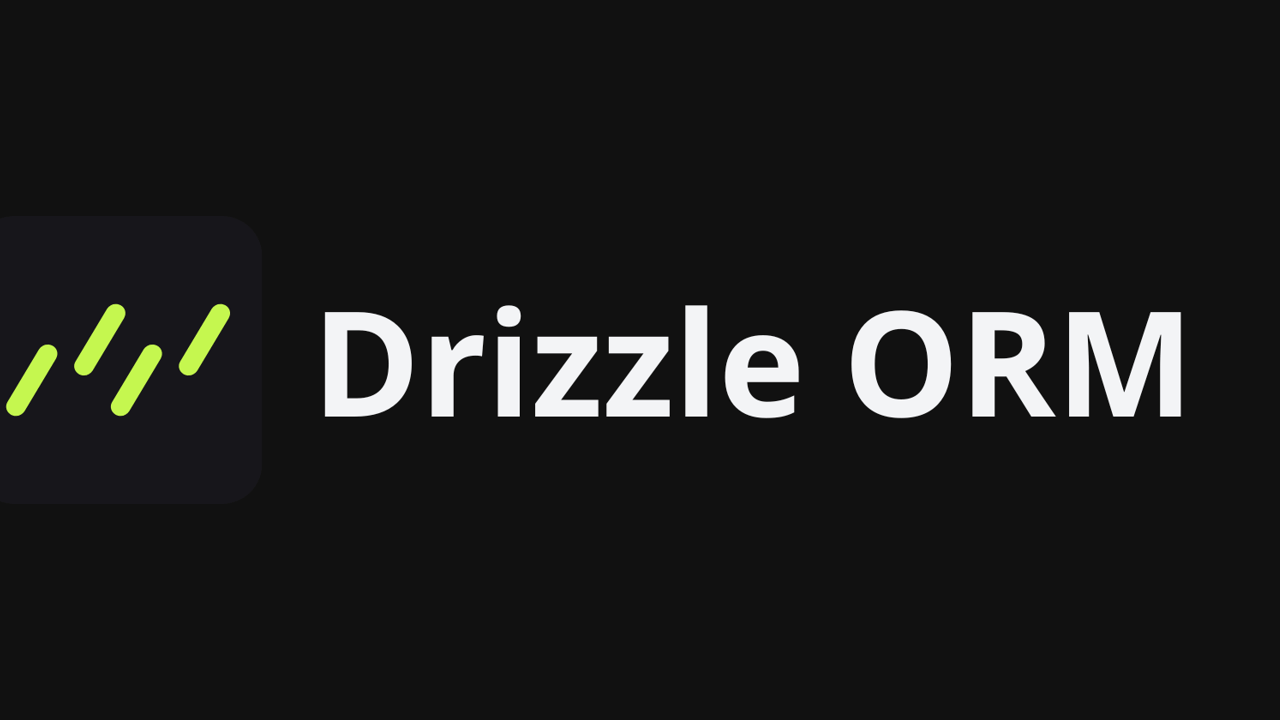
\includegraphics[width=0.85\textwidth,height=0.4\textheight,keepaspectratio]{images/postgresql_drizzle.png}
    \caption{PostgreSQL and Drizzle ORM Stack}
    \label{fig:postgres_drizzle}
\end{figure}

Figure~\ref{fig:postgres_drizzle} shows how PostgreSQL and Drizzle ORM fit together in Riaya.

\subsection{Voice Server and Real-Time: Express.js, Twilio, OpenAI Realtime API (Microsoft Azure)}
The voice server is built with \textbf{Express.js} \cite{express2024}, a minimalist Node.js framework for web applications and APIs, chosen for its simplicity, its performance, and its compatibility with WebSocket libraries such as \texttt{ws}.

\textbf{Twilio} \cite{twilio2024} receives the patients' phone calls. When a patient dials the Riaya number, Twilio sends a webhook to the Express.js server, which answers with TwiML (Twilio Markup Language) that opens a WebSocket media stream from Twilio to the server. Through this stream, the server receives live audio from the patient's phone and sends audio back.

The AI voice agent runs on the \textbf{OpenAI Realtime API} \cite{openai2024realtime}, accessed through \textbf{Microsoft Azure} \cite{azure2024openai}. Its speech-to-speech mode lets the AI understand the patient and answer in real time. The agent speaks English, French, and Tunisian Arabic, and it calls tools in the Riaya system to search for doctors, check availability, and create appointments. Azure was chosen as the host because its regional deployments reduce network latency for users in North Africa.

\begin{figure}[H]
    \centering
    \begin{subfigure}[b]{0.22\textwidth}
        \centering
        
\includegraphics[width=\textwidth,height=2.2cm,keepaspectratio]{images/expressjs.png}
        \caption{Express.js}
        \label{fig:logo_express}
    \end{subfigure}
    \hfill
    \begin{subfigure}[b]{0.22\textwidth}
        \centering
        
\includegraphics[width=\textwidth,height=2.2cm,keepaspectratio]{images/twilio.png}
        \caption{Twilio}
        \label{fig:logo_twilio}
    \end{subfigure}
    \hfill
    \begin{subfigure}[b]{0.22\textwidth}
        \centering
        
\includegraphics[width=\textwidth,height=2.2cm,keepaspectratio]{images/openai.png}
        \caption{OpenAI}
        \label{fig:logo_openai}
    \end{subfigure}
    \hfill
    \begin{subfigure}[b]{0.22\textwidth}
        \centering
        
\includegraphics[width=\textwidth,height=2.2cm,keepaspectratio]{images/azure.png}
        \caption{Microsoft Azure}
        \label{fig:logo_azure}
    \end{subfigure}
    \caption{Logos of the voice server and real-time communication technologies}
    \label{fig:logos_voice}
\end{figure}

\begin{figure}[H]
    \centering
    
\includegraphics[width=0.85\textwidth,height=0.4\textheight,keepaspectratio]{images/voice_server_stack.png}
    \caption{Voice Server and Real-Time Stack}
    \label{fig:voice_stack}
\end{figure}

Figures~\ref{fig:logos_voice} and~\ref{fig:voice_stack} present the voice server stack.

\subsection{Third-Party Integrations: WhatsApp Baileys, Cloudflare R2, Konnect.network}
\textbf{WhatsApp Baileys} \cite{baileys2024} is a library that connects to WhatsApp Web and sends messages from code. Doctors link their own WhatsApp number by scanning a QR code, so every message goes out from the doctor's own number and the conversation between doctor and patient stays private.

\textbf{Cloudflare R2} \cite{cloudflare2024r2} stores uploaded medical documents and files. It is S3-compatible object storage with low latency, high durability, and no egress fees.

\textbf{Konnect.network} \cite{konnect2024} processes the Pro plan payments, including the recurring invoices generated by a daily BullMQ job.

\begin{figure}[H]
    \centering
    \begin{subfigure}[b]{0.3\textwidth}
        \centering
        
\includegraphics[width=\textwidth,height=2.5cm,keepaspectratio]{images/whatsapp.png}
        \caption{WhatsApp Baileys}
        \label{fig:logo_whatsapp}
    \end{subfigure}
    \hfill
    \begin{subfigure}[b]{0.3\textwidth}
        \centering
        
\includegraphics[width=\textwidth,height=2.5cm,keepaspectratio]{images/cloudflare.png}
        \caption{Cloudflare R2}
        \label{fig:logo_cloudflare}
    \end{subfigure}
    \hfill
    \begin{subfigure}[b]{0.3\textwidth}
        \centering
        
\includegraphics[width=\textwidth,height=2.5cm,keepaspectratio]{images/konnect.png}
        \caption{Konnect.network}
        \label{fig:logo_konnect}
    \end{subfigure}
    \caption{Logos of the third-party integrations}
    \label{fig:logos_thirdparty}
\end{figure}

Figure~\ref{fig:logos_thirdparty} shows the logos of the third-party integrations.

\subsection{Background Jobs and Cache: BullMQ, Redis}
\textbf{BullMQ} \cite{bullmq2024} is a Node.js library for background jobs and scheduled tasks. It runs on \textbf{Redis} \cite{redis2024}, an in-memory data store used for caching and message brokering. In Riaya, BullMQ handles several critical tasks:
\begin{itemize}
    \item Sending a WhatsApp review message two hours after a confirmed appointment ends.
    \item Generating recurring invoices for Pro subscriptions that are about to expire.
    \item Handling timeouts for pending appointments (auto-cancellation after 10 minutes).
    \item Sending callbacks or WhatsApp notifications to patients when a pending request expires.
\end{itemize}

The team chose BullMQ over simpler options such as node-cron for its reliability, retry policies, and observability. Its dashboard shows job status in real time.

\begin{figure}[H]
    \centering
    \begin{subfigure}[b]{0.3\textwidth}
        \centering
        
\includegraphics[width=\textwidth,height=2.5cm,keepaspectratio]{images/bullmq.png}
        \caption{BullMQ}
        \label{fig:logo_bullmq}
    \end{subfigure}
    \hfill
    \begin{subfigure}[b]{0.3\textwidth}
        \centering
        
\includegraphics[width=\textwidth,height=2.5cm,keepaspectratio]{images/redis.png}
        \caption{Redis}
        \label{fig:logo_redis}
    \end{subfigure}
    \caption{Logos of the background jobs and cache technologies}
    \label{fig:logos_background}
\end{figure}

\begin{figure}[H]
    \centering
    
\includegraphics[width=0.8\textwidth,height=0.4\textheight,keepaspectratio]{images/bullmq_redis.png}
    \caption{Background Jobs and Cache Stack (BullMQ and Redis)}
    \label{fig:bullmq_redis}
\end{figure}

Figures~\ref{fig:logos_background} and~\ref{fig:bullmq_redis} present the background jobs and cache stack.

\subsection{Infrastructure and CI/CD: Docker, GitHub Actions, Ubuntu VPS, Nginx}
Riaya runs in \textbf{Docker} \cite{docker2024} containers managed by \textbf{Docker Compose} on a self-hosted \textbf{Ubuntu VPS}. Each repository has its own \textbf{GitHub Actions} CI/CD workflow: on every push to the \texttt{main} branch, GitHub-hosted runners build the Docker images, publish them to the \textbf{GitHub Container Registry (GHCR)}, and deploy the updated containers to the VPS.

On the VPS, \textbf{Nginx} acts as a reverse proxy in front of the application containers and handles TLS termination and routing. PostgreSQL and Redis run as containers on a shared Docker network, which the web and voice containers join. Web deployments run the Drizzle migrations before the new container starts. This setup follows the continuous delivery principles of Humble and Farley \cite{humble2010continuous}.

\begin{figure}[H]
    \centering
    \begin{subfigure}[b]{0.22\textwidth}
        \centering
        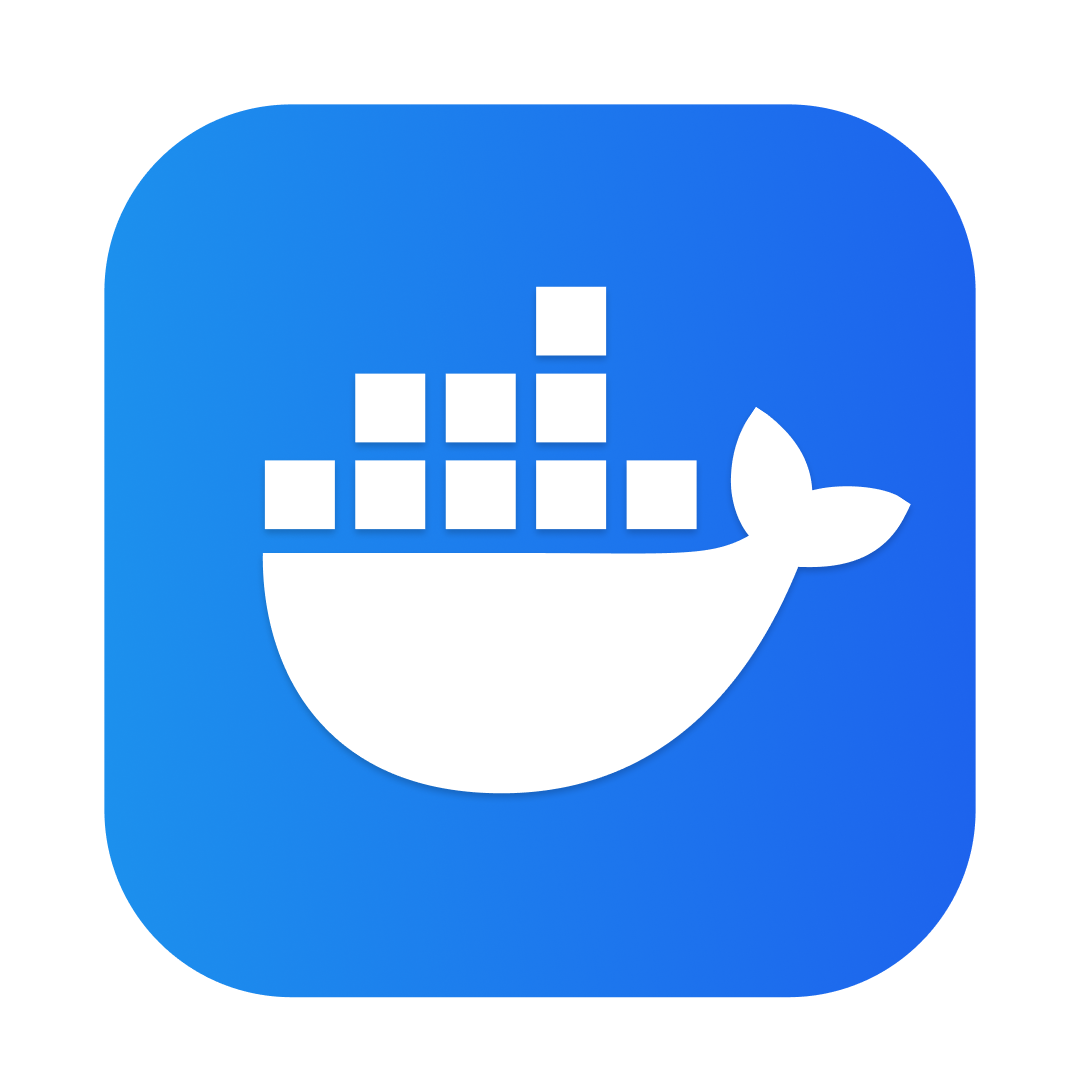
\includegraphics[width=\textwidth,height=2.2cm,keepaspectratio]{images/docker.png}
        \caption{Docker}
        \label{fig:logo_docker}
    \end{subfigure}
    \hfill
    \begin{subfigure}[b]{0.22\textwidth}
        \centering
        
\includegraphics[width=\textwidth,height=2.2cm,keepaspectratio]{images/github-actions.png}
        \caption{GitHub Actions}
        \label{fig:logo_ghactions}
    \end{subfigure}
    \hfill
    \begin{subfigure}[b]{0.22\textwidth}
        \centering
        
\includegraphics[width=\textwidth,height=2.2cm,keepaspectratio]{images/ubuntu.png}
        \caption{Ubuntu}
        \label{fig:logo_ubuntu}
    \end{subfigure}
    \hfill
    \begin{subfigure}[b]{0.22\textwidth}
        \centering
        
\includegraphics[width=\textwidth,height=2.2cm,keepaspectratio]{images/nginx.png}
        \caption{Nginx}
        \label{fig:logo_nginx}
    \end{subfigure}
    \caption{Logos of the infrastructure and CI/CD technologies}
    \label{fig:logos_infra}
\end{figure}

Figure~\ref{fig:logos_infra} presents the logos of the infrastructure and CI/CD technologies.

\section{Screenshots and Detailed Descriptions}
This section shows the main screens of Riaya, grouped by interface, with a description of what each one does. Together they show how the functional requirements of Chapter~1 were implemented.

\subsection{Admin Interface: Dashboard and Statistics}
The admin home page gives an overview of the whole platform. It shows key statistics, such as the number of registered doctors, appointments, and AI calls, along with charts of platform trends, doctor activity, and usage.

\IfFileExists{images/admin_dashboard_home.png}{%
\begin{figure}[H]
    \centering
    \includegraphics[width=0.85\textwidth,height=0.5\textheight,keepaspectratio]{images/admin_dashboard_home.png}
    \caption{Admin Dashboard Home Page}
    \label{fig:admin_home}
\end{figure}
}{}

\subsection{Doctor Interface: Appointment Calendar and Urgent Badges}
Doctors see and manage their schedule in a calendar view. New AI requests appear in real time over WebSockets. Urgent requests carry a badge and trigger a stronger live notification for the doctor, which the urgent booking flow described in Section~\ref{subsec:urgencies} depends on.

\begin{figure}[H]
    \centering
    
\includegraphics[width=0.85\textwidth,height=0.5\textheight,keepaspectratio]{images/doctor_calendar.png}
    \caption{Doctor Appointment Calendar with Urgent Badges}
    \label{fig:doctor_calendar}
\end{figure}

Figure~\ref{fig:doctor_calendar} shows the doctor's appointment calendar with urgent badges.

\subsection{Doctor Interface: WhatsApp Configuration and QR Code Generation}
On this page, doctors link their personal WhatsApp number by scanning a QR code. Once connected, every message goes out from the doctor's own number, which keeps conversations private. The page also shows the connection status and lets the doctor disconnect the session.

\begin{figure}[H]
    \centering
    
\includegraphics[width=0.85\textwidth,height=0.5\textheight,keepaspectratio]{images/doctor_whatsapp_config.png}
    \caption{WhatsApp Configuration Page with QR Code}
    \label{fig:doctor_whatsapp}
\end{figure}

Figure~\ref{fig:doctor_whatsapp} shows the WhatsApp configuration page with QR code generation.

\subsection{Doctor Interface: Invoice Management and WhatsApp Sending}
Doctors create, edit, and cancel invoices on this page, and send an invoice to the patient on WhatsApp with one click. The page also shows the payment status (paid or unpaid) and the invoice history.

\begin{figure}[H]
    \centering
    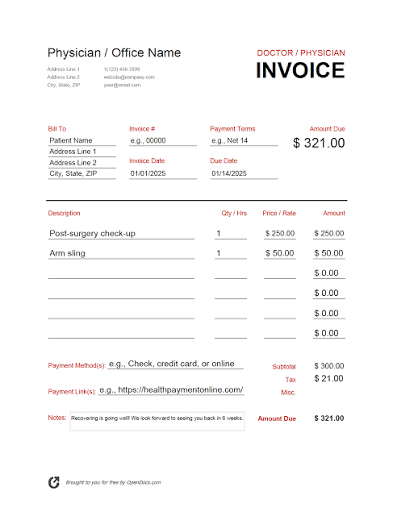
\includegraphics[width=0.85\textwidth,height=0.5\textheight,keepaspectratio]{images/doctor_invoice.png}
    \caption{Invoice Management Page}
    \label{fig:doctor_invoice}
\end{figure}

Figure~\ref{fig:doctor_invoice} shows the invoice management page.

\subsection{Admin Interface: Live Call Monitoring and Transcriptions}
On this page, administrators follow ongoing calls between the AI agent and patients in real time. It shows the live transcript, the patient's name, and the call status, which the team relies on for operations and debugging.

\begin{figure}[H]
    \centering
    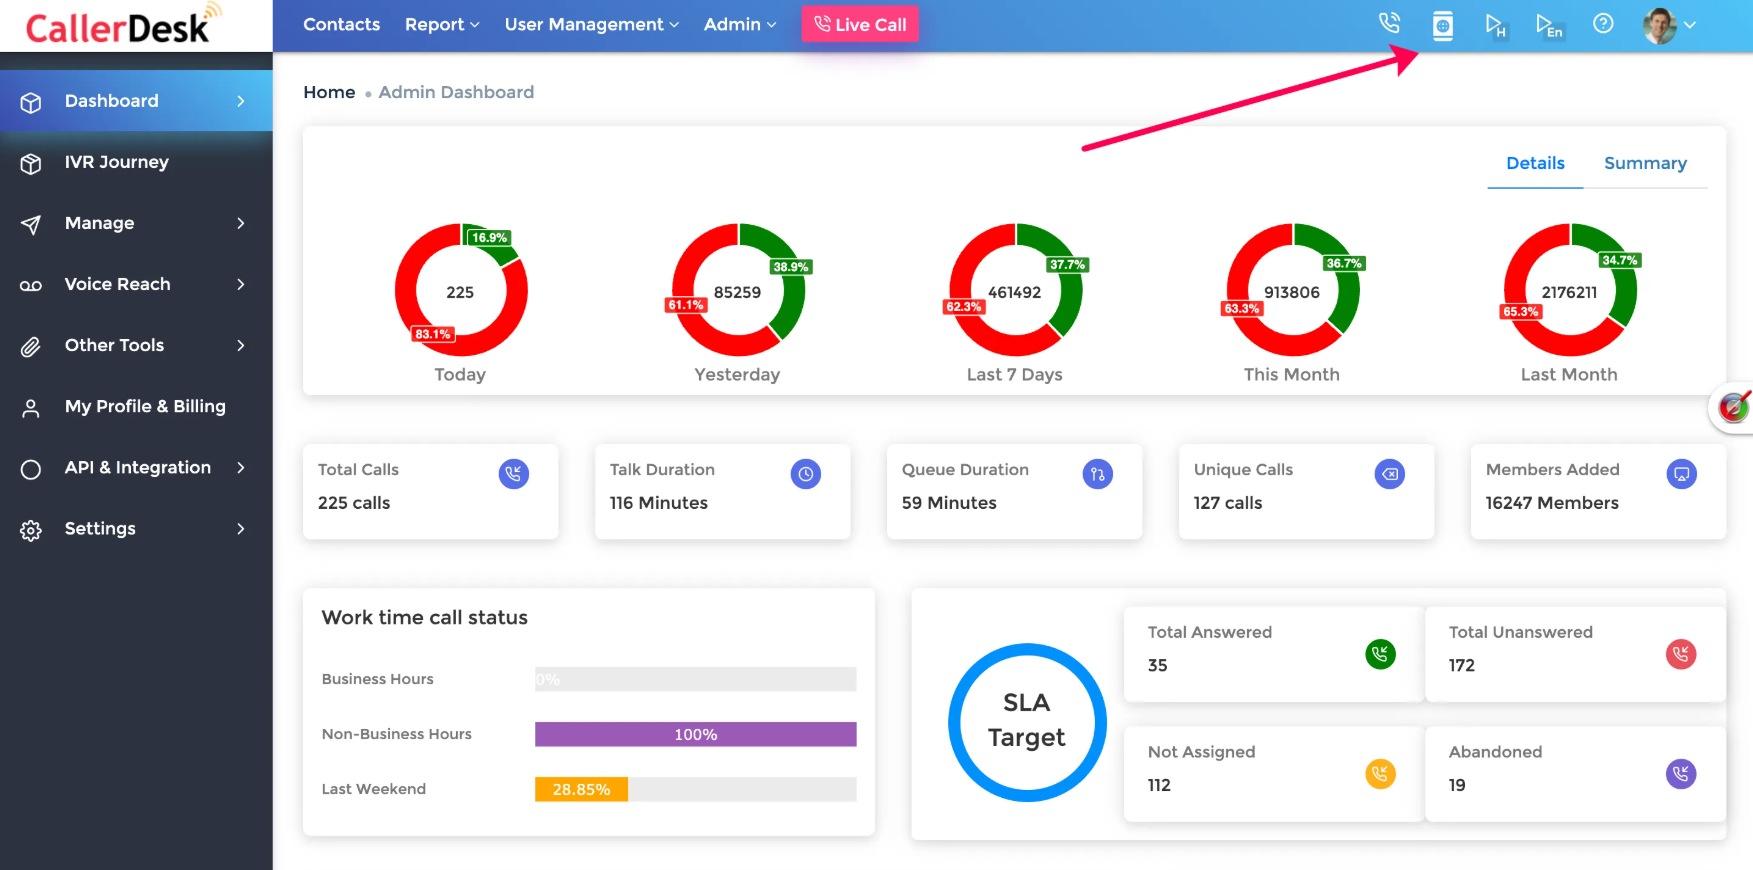
\includegraphics[width=0.85\textwidth,height=0.5\textheight,keepaspectratio]{images/admin_live_call.png}
    \caption{Admin Live Call Monitoring Interface}
    \label{fig:admin_live_call}
\end{figure}

Figure~\ref{fig:admin_live_call} shows the admin live call monitoring interface.

\subsection{Admin Interface: Doctor Verification and Best-Fit Search}
On the doctor verification page, administrators browse and search doctor applications and approve or reject them, optionally with reasons shown to the doctor. The best-fit search page runs the same search algorithm the AI uses, so administrators can check on a map and a calendar which doctors match a speciality, location, and date range.

\begin{figure}[H]
    \centering
    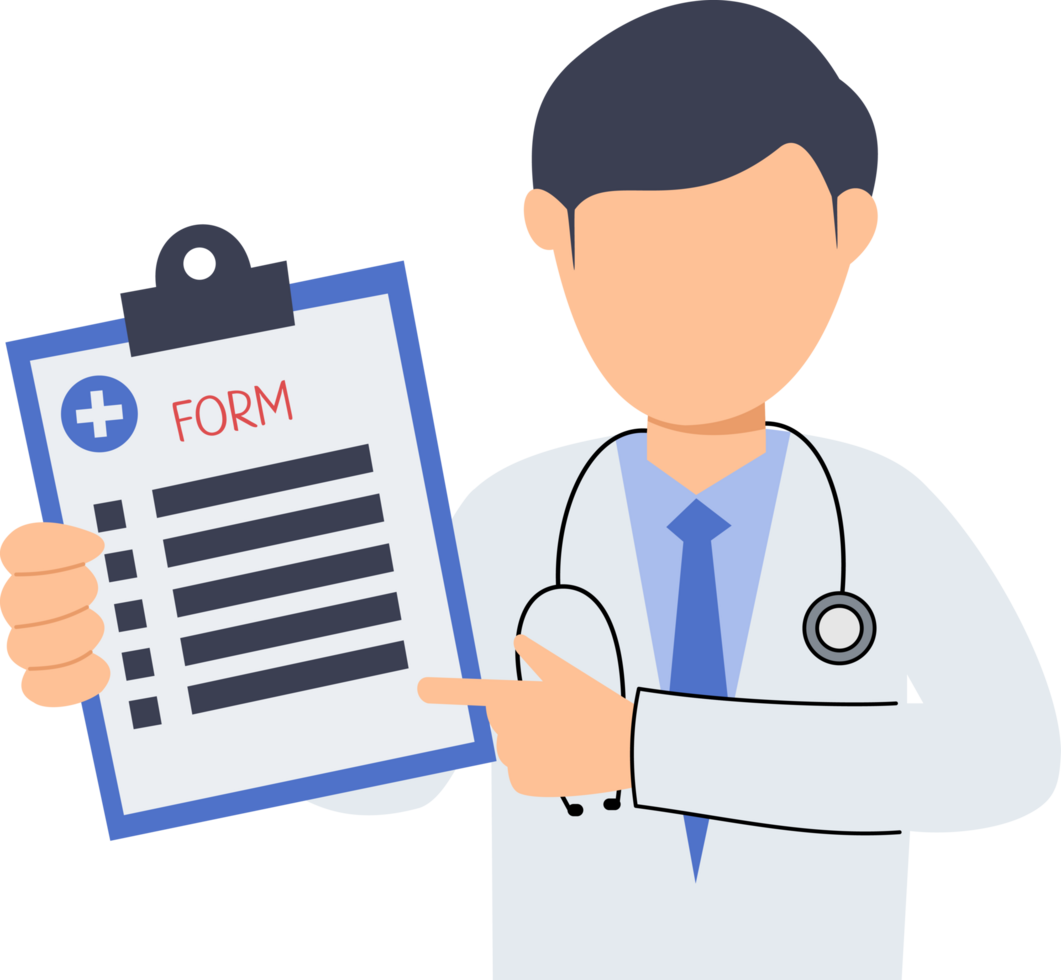
\includegraphics[width=0.85\textwidth,height=0.5\textheight,keepaspectratio]{images/admin_doctor_verification.png}
    \caption{Admin Doctor Verification Interface}
    \label{fig:admin_verification}
\end{figure}

\begin{figure}[H]
    \centering
    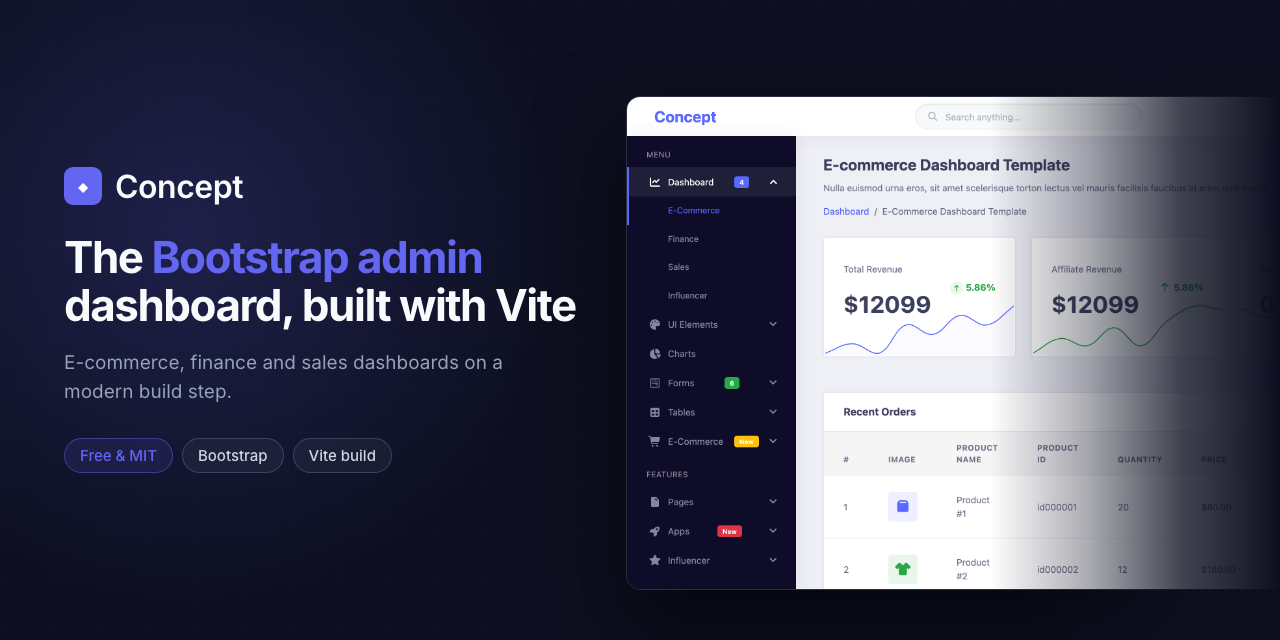
\includegraphics[width=0.85\textwidth,height=0.5\textheight,keepaspectratio]{images/admin_bestfit_search.png}
    \caption{Admin Best-Fit Search Interface}
    \label{fig:admin_bestfit}
\end{figure}

Figures~\ref{fig:admin_verification} and~\ref{fig:admin_bestfit} show the doctor verification and best-fit search interfaces.

\subsection{Database: ERD Diagram and Drizzle Migrations}
The ERD shows the database schema, and the terminal output shows the Drizzle migration files running during deployment.

\begin{figure}[H]
    \centering
    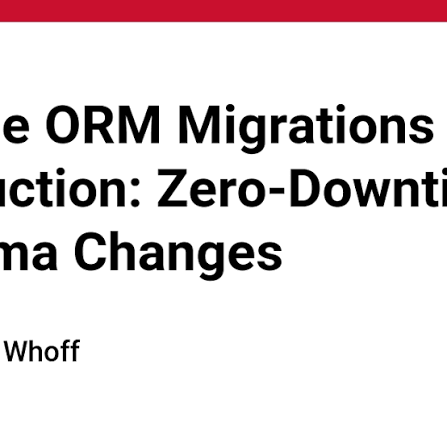
\includegraphics[width=0.85\textwidth,height=0.5\textheight,keepaspectratio]{images/erd_diagram_ch3.png}
    \caption{Entity-Relationship Diagram of the Riaya Database}
    \label{fig:erd_ch3}
\end{figure}

\begin{figure}[H]
    \centering
    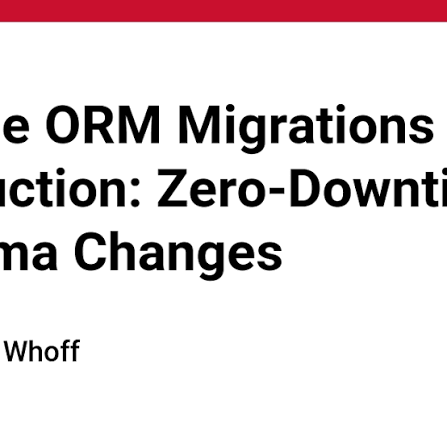
\includegraphics[width=0.85\textwidth,height=0.5\textheight,keepaspectratio]{images/drizzle_migrations.png}
    \caption{Drizzle Migrations Execution}
    \label{fig:drizzle_migrations}
\end{figure}

Figures~\ref{fig:erd_ch3} and~\ref{fig:drizzle_migrations} show the ERD and the Drizzle migrations.

\subsection{Twilio Console: Call Logs and Webhooks}
The Twilio console lists incoming calls and the webhooks that point to the Express.js voice server.

\begin{figure}[H]
    \centering
    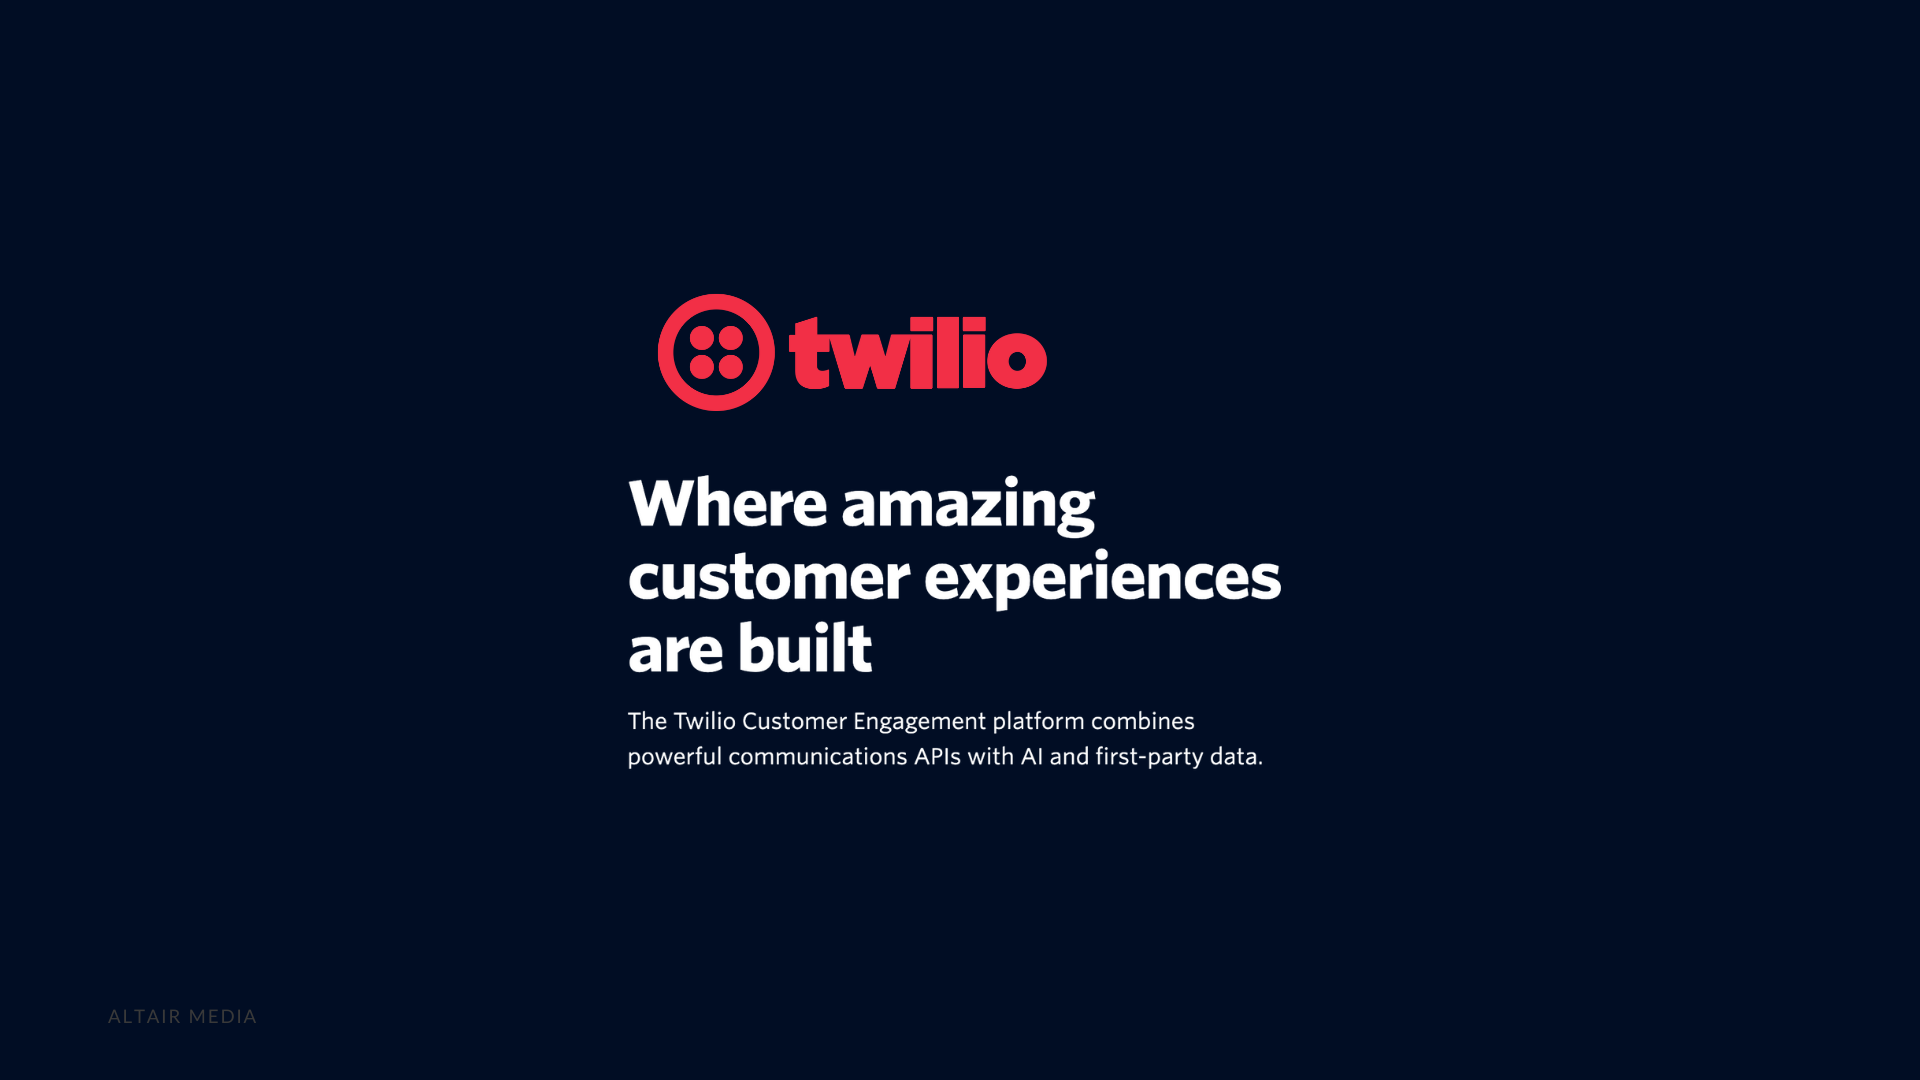
\includegraphics[width=0.85\textwidth,height=0.5\textheight,keepaspectratio]{images/twilio_console.png}
    \caption{Twilio Console with Call Logs and Webhooks}
    \label{fig:twilio_console}
\end{figure}

Figure~\ref{fig:twilio_console} shows the Twilio console with call logs and webhooks.

\subsection{Azure / OpenAI Portal: Voice Agent Configuration}
The Azure portal shows the deployment of the OpenAI Realtime model behind the AI voice agent and its configuration, including the language settings and the tool definitions.

\begin{figure}[H]
    \centering
    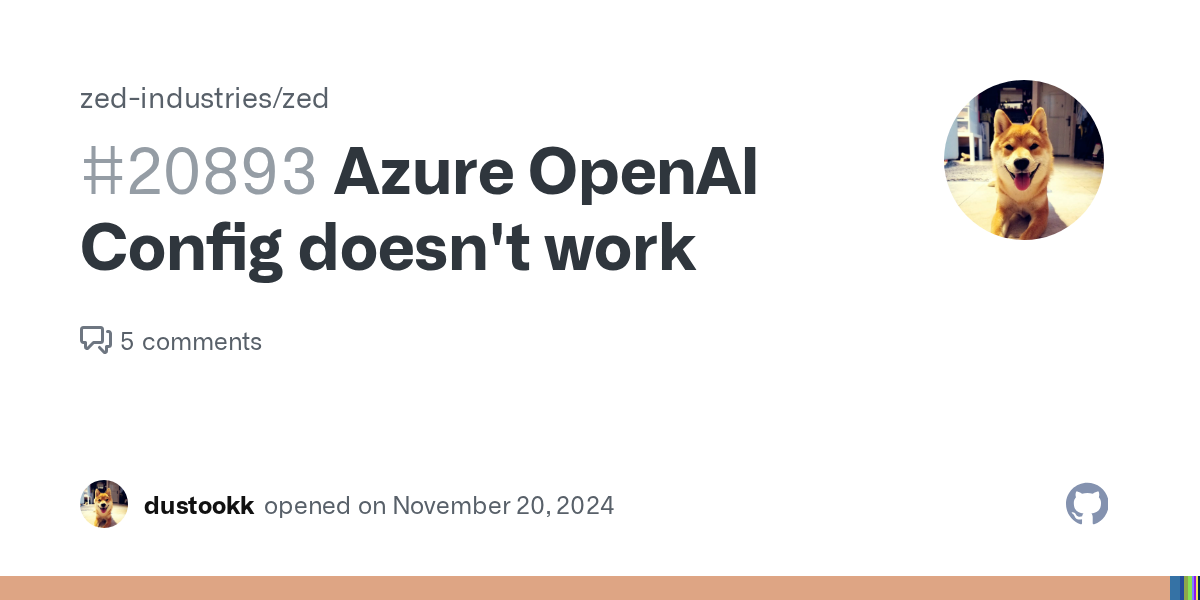
\includegraphics[width=0.85\textwidth,height=0.5\textheight,keepaspectratio]{images/azure_openai_config.png}
    \caption{Azure / OpenAI Portal Configuration}
    \label{fig:azure_openai}
\end{figure}

Figure~\ref{fig:azure_openai} shows the Azure / OpenAI portal configuration.

\subsection{BullMQ Dashboard (Redis Insight): Scheduled Jobs Monitoring}
The BullMQ dashboard, opened through Redis Insight, lists the scheduled jobs and their status (waiting, active, completed, failed). The team uses it to monitor background tasks such as review requests and recurring invoices.

\begin{figure}[H]
    \centering
    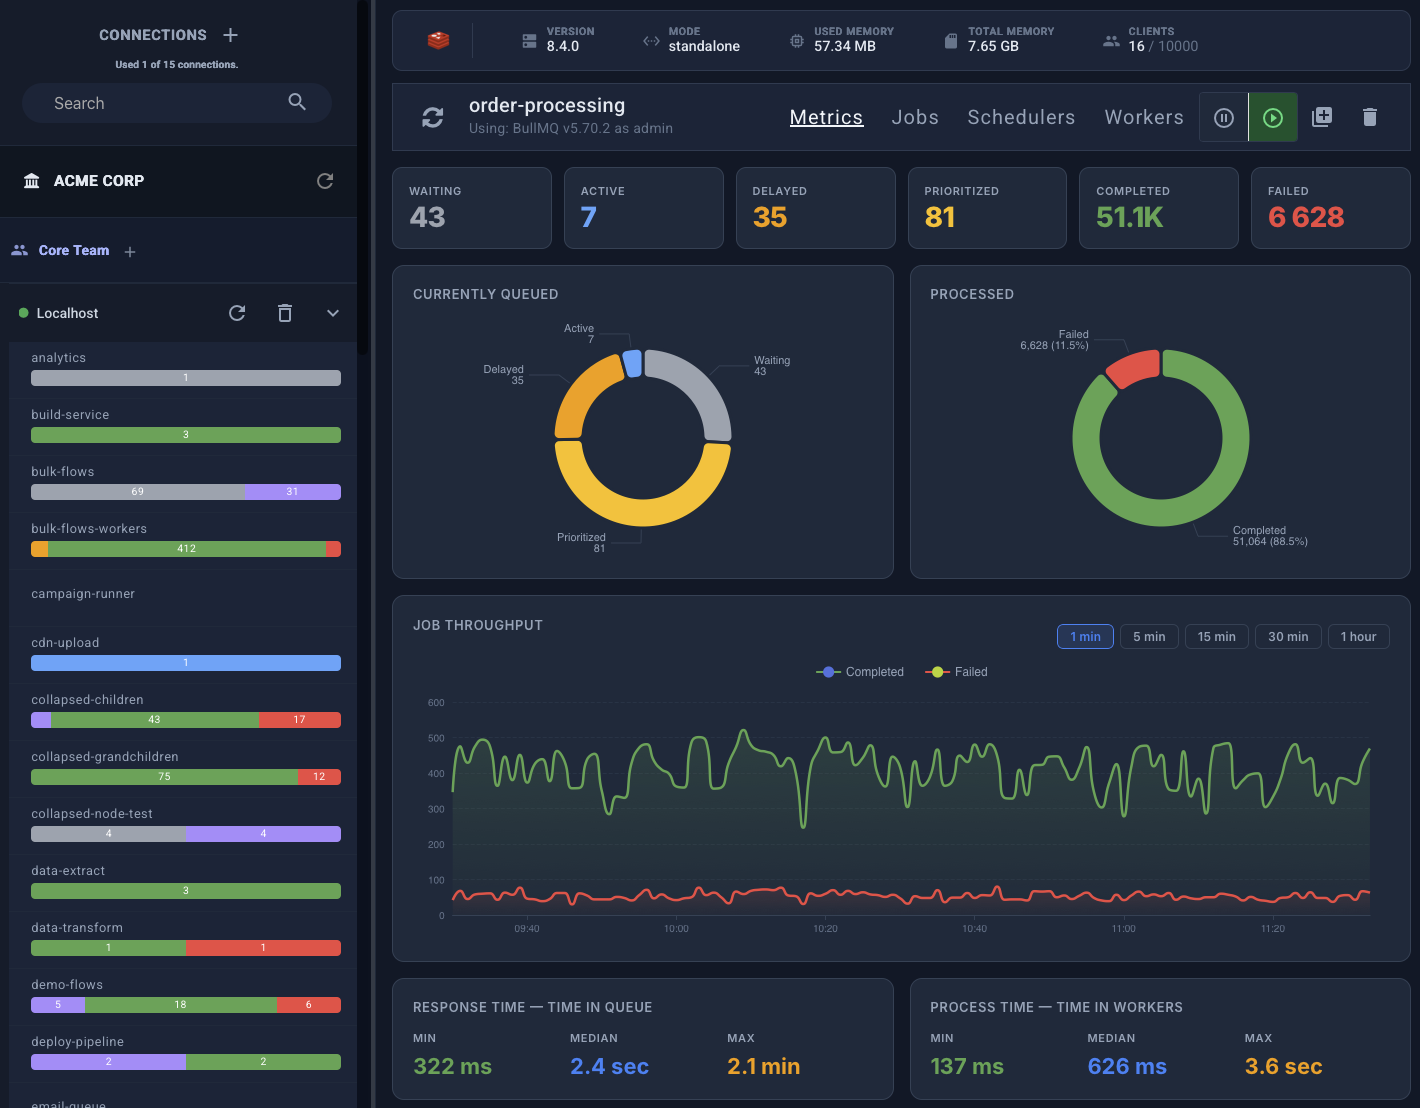
\includegraphics[width=0.85\textwidth,height=0.5\textheight,keepaspectratio]{images/bullmq_dashboard.png}
    \caption{BullMQ Dashboard for Scheduled Jobs}
    \label{fig:bullmq_dashboard}
\end{figure}

Figure~\ref{fig:bullmq_dashboard} shows the BullMQ dashboard for scheduled jobs.

\subsection{WhatsApp Baileys Logs: Connection and Message Sending}
The WhatsApp Baileys logs show the connection status of the doctor's WhatsApp session and each message as it is sent.

\begin{figure}[H]
    \centering
    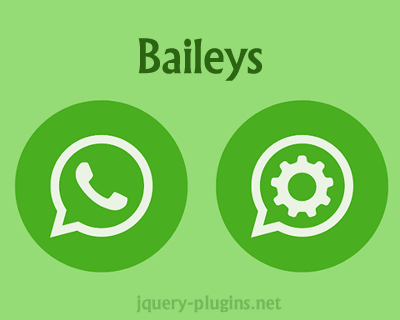
\includegraphics[width=0.85\textwidth,height=0.5\textheight,keepaspectratio]{images/whatsapp_baileys_logs.png}
    \caption{WhatsApp Baileys Connection and Message Logs}
    \label{fig:whatsapp_logs}
\end{figure}

Figure~\ref{fig:whatsapp_logs} shows the WhatsApp Baileys connection and message logs.

\subsection{GitHub Actions: CI/CD Workflow}
The GitHub Actions workflow shows each step of the automated CI/CD pipeline: building the Docker image, publishing it to GHCR, and deploying it to the VPS.

\begin{figure}[H]
    \centering
    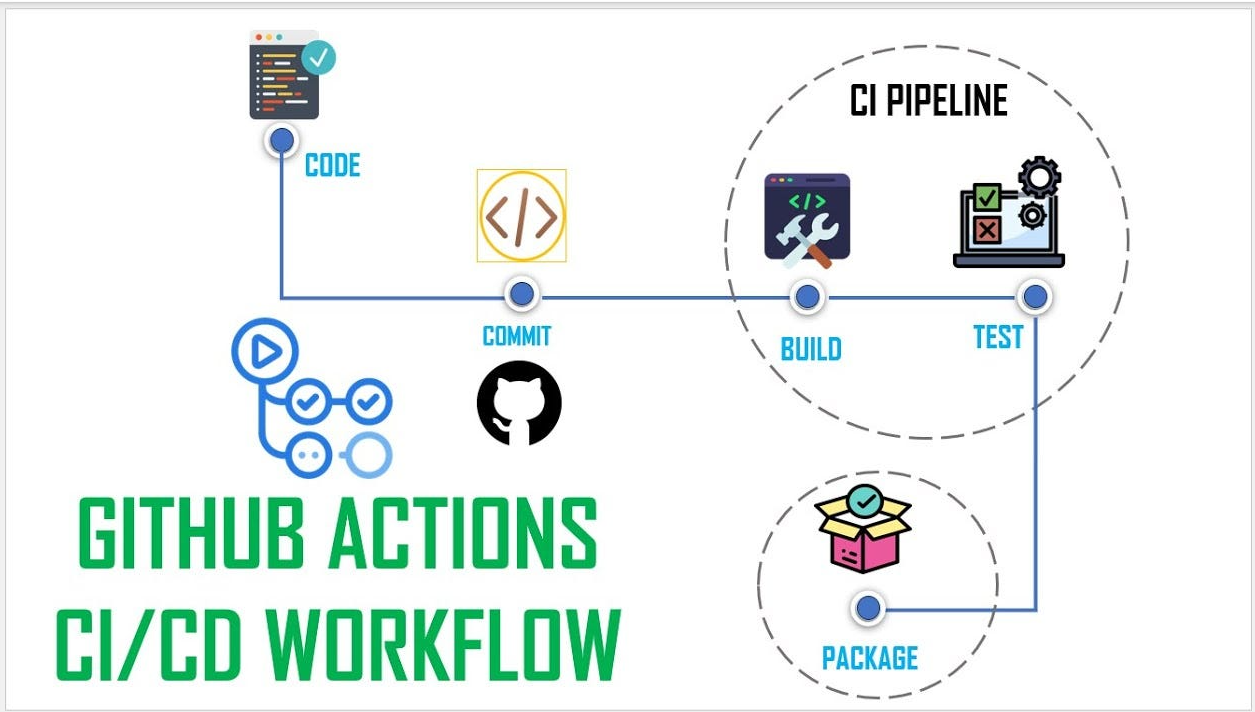
\includegraphics[width=0.85\textwidth,height=0.5\textheight,keepaspectratio]{images/github_actions_workflow.png}
    \caption{GitHub Actions CI/CD Workflow}
    \label{fig:github_actions}
\end{figure}

Figure~\ref{fig:github_actions} shows the GitHub Actions CI/CD workflow.

\subsection{Docker Compose: Running Containers on the VPS}
The Docker Compose output lists the containers running on the VPS (the web app, the voice server, PostgreSQL, Redis, and Nginx) and their health.

\begin{figure}[H]
    \centering
    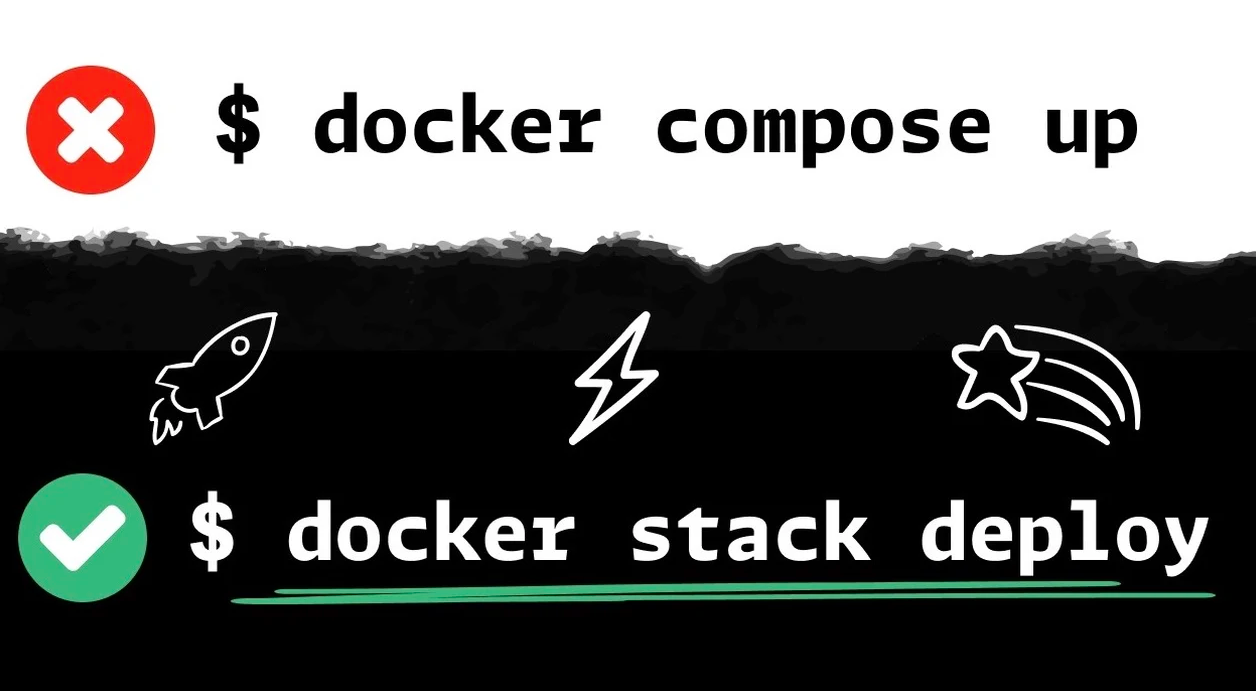
\includegraphics[width=0.85\textwidth,height=0.5\textheight,keepaspectratio]{images/docker_compose_vps.png}
    \caption{Docker Compose Running Containers on the VPS}
    \label{fig:docker_compose}
\end{figure}

Figure~\ref{fig:docker_compose} shows the Docker Compose output with running containers on the VPS.

\section{Security, Confidentiality, and Access Management}

\subsection{Authentication and Authorization (OTP, Better Auth, Roles)}
Better Auth handles authentication, with support for email and password, OTP, and session management. Doctors must verify their email with an OTP sent by Nodemailer before they can complete registration, and until an administrator approves the application, they can only reach the profile page. Authorization is role-based: doctors, administrators, and patients (who have no account) each have a different level of access. This follows the principle of least privilege recommended by OWASP \cite{owasp2024}.

\begin{table}[H]
    \centering
    \caption{Authentication and Authorization Matrix}
    \label{tab:auth_matrix}
    \small
    \begin{tabular}{p{2.5cm}p{3.5cm}p{3.5cm}p{3.5cm}}
        \toprule
        \textbf{Role} & \textbf{Authentication} & \textbf{Access Level} & \textbf{Restrictions} \\
        \midrule
        Patient & None (phone number) & Phone call + WhatsApp & No web access \\
        Doctor & Email OTP (Better Auth) & Full dashboard after approval & Profile only until approved \\
        Administrator & Email and password & Full back-office access & None \\
        \bottomrule
    \end{tabular}
\end{table}

Table~\ref{tab:auth_matrix} summarizes how each role authenticates and what it can access.

\subsection{Protection of Medical Data (Cloudflare R2, Compliance)}
Medical documents are stored in Cloudflare R2, which encrypts them at rest and in transit. Access is restricted to the doctor who uploaded a document and, where applicable, to the patient through WhatsApp. The platform must comply with Tunisian data protection regulations (INPDP) \cite{inpdp2004} and, where applicable, with the GDPR principles \cite{gdpr2016} of data minimization, purpose limitation, and the right to erasure. The team chose Cloudflare R2 for its S3-compatible API, its strong encryption, and its zero egress fees, which keep down the cost of storing large medical files.

\subsection{Confidentiality of WhatsApp Conversations}
WhatsApp messages go out through the doctor's own phone number (via WhatsApp Baileys), so the conversation between doctor and patient stays private, and Riaya has no access to the content of these messages once they are sent. The team chose this design to protect patient privacy and meet medical confidentiality requirements. It also spares the platform the data retention obligations it would have if it stored the messages itself.

\section{Technical Challenges Encountered and Solutions Adopted}

\subsection{Real-Time Latency Management (WebSockets, OpenAI Realtime)}
Latency was one of the main technical challenges. The voice server must relay audio between Twilio and the OpenAI Realtime API with minimal delay, or the conversation stops feeling natural. The team used WebSockets for low-latency communication, tuned the audio buffering strategy, and relied on Microsoft Azure's regional deployments to cut network latency. The target was under 500 ms end to end, the threshold usually given for natural conversation \cite{itu2003g114}.

\subsection{Best-Fit Algorithm (Haversine, Geoapify, Scoring)}
The best-fit algorithm was another hard problem. It has to resolve the patient's location, rank doctors by distance and availability, and return the top 2--3 options quickly. The team used Geoapify \cite{geoapify2024} for geocoding, the Haversine formula \cite{haversine1971} for distances, and a scoring function that combines distance and time difference. The algorithm is optimized to run within a few hundred milliseconds, so the patient is not kept waiting.

The scoring function is:
\[
\text{Score} = \text{distance (km)} + \frac{|\text{slot} - \text{preferred time}| \text{ (minutes)}}{10}
\]

\paragraph{Geocoding and Tunisian Locations.}
To find the patient's location, the platform uses Geoapify, which had the richest data among the services tested. It still has gaps: some addresses exist in several places, which makes them ambiguous. To compensate, the AI also receives a curated list of Tunisian cities and places, which helps it interpret what callers say and makes the best-fit search more accurate.

\subsection{Management of Urgencies and Timeouts}\label{subsec:urgencies}
The urgent booking flow and the timeout handling needed careful design. When the AI detects an urgent situation, it creates up to three pending appointments linked by an emergency group ID. The first doctor to accept gets the appointment, and the other requests are cancelled automatically. If no doctor accepts within 10 minutes, the whole group is cancelled and the patient is notified by a callback or a WhatsApp message. BullMQ schedules these tasks, and Redis holds their state. The mechanism draws on patterns from \textit{Enterprise Integration Patterns} \cite{hohpe2003eip}.

\subsection{Rejection Handling Workflow}
\label{subsec:rejection-handling}

One of the trickiest parts of the patient experience was deciding what happens when a doctor refuses an appointment or takes too long to answer. The team first considered asking the patient to choose a backup doctor up front, in case the first one refuses, but that would add yet another question to an already long call. The team chose a simpler approach: the patient picks one doctor, and if that doctor refuses, the platform calls the patient back with another option. This keeps the call as easy as possible for the patient. The team plans to test the approach further and may revise it if a better alternative appears.

\subsection{Pricing Display Decision}
\label{subsec:pricing-display}

Price matters when choosing a doctor, and the team first wanted to show prices on the platform. If only the first consultation price mattered, this would be easy. But the real cost depends on many factors, and two doctors with the same first consultation price can charge very different amounts for their services. The team considered letting doctors enter a price for each service, which works for services with a fixed price, such as braces. In most cases, though, patients do not know what they need before a diagnosis, and an AI cannot reliably handle a diagnosis over the phone. The team therefore decided not to show full prices, so patients are not misled and the platform stays focused on booking rather than medical pricing.

\subsection{Voice Model Evaluation and Selection}
\label{subsec:voice-model-evaluation}

The phone call is the most important feature of Riaya, so the team put a lot of effort into choosing the AI models and the architecture behind it. This section covers the two main ways to build an AI phone call, the testing method, the problem of Tunisian Arabic, the approaches tested, the results, and the final choice.

\subsubsection{Two Approaches to Build a Phone Call}
There are two fundamentally different ways to build an AI-powered phone call. The first is \emph{speech-to-speech} (realtime): a single model listens to the caller and answers with its own voice. This approach is fast and feels natural. The second is a \emph{chain of steps}: the caller's voice is converted to text (STT), an AI model generates the answer (LLM), and the answer is converted back to voice (TTS). This gives more control because the best model can be chosen for each step, but every step adds waiting time. The team tested both approaches.

\subsubsection{Testing Methodology}
The team built a small program that acts like a phone caller. It plays the same seven sentences each time, covering Tunisian Arabic, French, and mixed sentences such as \textit{``\foreignlanguage{arabic}{نحب ناخذ} rendez-vous \foreignlanguage{arabic}{عند} dermatologue''}. The program records the AI's answers and measures the response time. The real application instructions and booking tools were used, so the AI behaved as it would in production. Each step was also timed individually to identify bottlenecks. To compare fairly, a test call page was built where the engine could be switched and the same call run on each one. One limitation: the test voices were computer-generated, not real patients.

\subsubsection{The Challenge of Tunisian Arabic}
For English and French, almost every speech-to-text and voice model tested performed well. Tunisian Arabic (Derja) was where the models differed significantly, and it was the main problem from the start. Few models understand it: one model returned nothing for Arabic, while others dropped or misspelled words. Mixed sentences with French words inside Arabic were the hardest. Few voices speak it well: Gemini had the most natural Arabic voices, while Inworld offered only two Arabic voices that were not perfect. Every choice was judged on Tunisian Arabic first, because that is how the patients speak.

\subsubsection{Approach 1: Realtime Models (Speech-to-Speech)}
The team started with Azure OpenAI Realtime and then tested Gemini Live for comparison. GPT Realtime had a very good response time and followed instructions well, but its pronunciation was not perfect. Gemini Live also had a very good response time and the best voice, but it could not follow instructions carefully and lost track of the conversation. The ``extended thinking'' version often failed to use the results of the booking tools (8 out of 18 tries in the test). On response time, both were fast: Gemini Live answered in 1.6 to 4.5 seconds, faster when answering immediately and slower when calling a tool first.

\subsubsection{Approach 2: Chain of Steps with Inworld.ai}
Next, the team tried the chain of steps, first with Inworld.ai. The AI models available there were not great, and it answered in about 2.2 seconds in the test call. Inworld also has only two Arabic voices, which were not perfect.

\subsubsection{Approach 3: LiveKit Agents with Different Models}
After that, LiveKit agents were used. They allow choosing the model for every step, so many combinations could be tested. The comparison table below comes from these tests. Inworld was mainly used as a speech-to-text and text-to-speech provider. Its speech-to-text was not good in Arabic, and its voice was not perfect either. No good combination of a good model and a fast response time was found.

\begin{table}[h]
\centering
\caption{Comparison of models tested in the chain of steps.}
\label{tab:voice-model-comparison}
\begin{tabular}{p{2.5cm}p{3cm}p{5cm}p{4cm}}
\hline
\textbf{Step} & \textbf{Model} & \textbf{What was found} & \textbf{Problem} \\
\hline
Listening & Microsoft MAI & Best on our sentences, about 0.5 s & A preview product, one provider only \\
Listening & Gemini & Excellent text & 2 to 3 s per sentence \\
Listening & Inworld & Fast & Not good in Arabic, worst on mixed sentences \\
Thinking & GPT-4o mini & Fast, about 1.2 s to start & Less smart than Claude \\
Thinking & Claude Sonnet & The smartest & 3 times slower to start (3.6 s) \\
Voice & Gemini & The most natural & 2 to 3 s before it starts talking \\
Voice & Inworld & Fast & Only 2 Arabic voices, not perfect \\
\hline
\end{tabular}
\end{table}

Table~\ref{tab:voice-model-comparison} summarizes the results of the model evaluation.

\subsubsection{Lessons Learned}
The tests taught the team three things. The best models were often the slowest: the best voice and the best listening model were both slow. Delays add up, because each step in the chain adds its own wait. And testing found real bugs. For example, the AI saved the caller's name or language on almost every turn, which cost about one extra second each time, so this was moved to a background job. Even so, the fastest chain the team built waited about 6.8 seconds before answering, and with Gemini for both listening and the voice, it took more than 10 seconds.

\subsubsection{Latency and Final Choice}
On a phone call, the wait between the caller finishing and the AI answering matters a lot: a long wait makes the call feel strange, so the team paid close attention to speed. GPT Realtime and Gemini Live both answered quickly. The Inworld setup was slower, at about 2.2 seconds, and the LiveKit chains were slower still, at 6.8 seconds or more. In the end, the team kept OpenAI Realtime, used directly from the OpenAI API, because it gave the best overall experience: fast answers and a smarter AI.

\section{Conclusion}
This chapter presented the technical architecture of Riaya: the split into two repositories, the technology stack, and the deployment infrastructure. It covered the web stack, the database, the voice server, the third-party integrations, the background jobs, and the CI/CD pipeline, showed the main features through screenshots, discussed security and confidentiality, and described the technical challenges and their solutions. The general conclusion that follows summarizes the work and presents future perspectives.
        \clearpage

        %% ============================================================
% CAPITOLO 5 : SVILUPPO PER SPRINT
% Versione ridotta (50%)
% ============================================================
\chapter{Sviluppo per Sprint}
\label{chap:sviluppo-sprint}

% ------------------------------------------------------------
% INTRODUZIONE AL CAPITOLO
% ------------------------------------------------------------
In questo capitolo viene presentato lo sviluppo dettagliato del progetto attraverso gli otto sprint previsti dalla roadmap. Per ciascuno sprint vengono descritti l'obiettivo, il backlog delle User Stories, i casi d'uso principali, l'implementazione e il bilancio. Il capitolo si conclude con una sintesi complessiva degli sprint (velocità del team, burndown chart e lezioni apprese).

% ============================================================
% SPRINT 0
% ============================================================
\section{Sprint 0 -- Configurazione dell'ambiente e fondazioni}
\label{sec:sprint0}

\subsection{Obiettivo e backlog}
\label{subsec:sprint0-obiettivo}

L'obiettivo dello Sprint 0 è predisporre l'ambiente di sviluppo (repository Git, progetto React/Node.js, database MongoDB) e mettere in piedi le fondazioni dell'autenticazione di base.

\begin{table}[H]
    \centering
    \caption{Backlog dello Sprint 0}
    \label{tab:sprint0-backlog}
    \renewcommand{\arraystretch}{1.3}
    \begin{tabular}{|p{1.8cm}|p{7cm}|p{2.5cm}|p{1.5cm}|}
        \hline
        \textbf{ID} & \textbf{User Story} & \textbf{Priorità} & \textbf{Stima} \\
        \hline
        US00-01 & Inizializzare il repository Git & Alta & 2 \\
        \hline
        US00-02 & Configurare l'ambiente Node.js & Alta & 3 \\
        \hline
        US00-03 & Inizializzare il progetto React & Alta & 3 \\
        \hline
        US00-04 & Configurare MongoDB & Alta & 3 \\
        \hline
        US00-05 & Implementare l'autenticazione di base & Alta & 5 \\
        \hline
    \end{tabular}
\end{table}

\subsection{Casi d'uso e diagrammi}
\label{subsec:sprint0-casi-uso}

I casi d'uso principali sono: \textit{Inizializzare il progetto}, \textit{Configurare la base di dati} e \textit{Mettere in piedi l'autenticazione di base}.

\begin{table}[H]
    \centering
    \caption{Sintesi dei casi d'uso -- Sprint 0}
    \label{tab:uc-sprint0}
    \renewcommand{\arraystretch}{1.3}
    \begin{tabular}{|p{3.5cm}|p{3cm}|p{7.5cm}|}
        \hline
        \textbf{Caso d'uso} & \textbf{Attore} & \textbf{Scenario nominale} \\
        \hline
        Inizializzare il progetto & Sviluppatore & Creazione repository, init Node.js/React, configurazione dipendenze \\
        \hline
        Configurare la base di dati & Sviluppatore & Configurazione connessione a MongoDB tramite Mongoose \\
        \hline
        Autenticazione di base & Sviluppatore & Implementazione JWT e bcrypt \\
        \hline
    \end{tabular}
\end{table}


\begin{figure}[H]
    \centering
    \includegraphics[width=0.85\textwidth]{images/sprint0_diagrammi.png}
    \caption{Diagrammi -- Sprint 0}
    \label{fig:diagrammi-sprint0}
\end{figure}

\subsection{Implementazione e bilancio}
\label{subsec:sprint0-implementazione}

Sono state implementate le configurazioni iniziali, la connessione al database e le fondazioni dell'autenticazione. Sono stati eseguiti test di connessione, generazione JWT e cifratura password. Lo sprint è stato completato con successo; le difficoltà principali hanno riguardato la configurazione iniziale dell'ambiente.

% ============================================================
% SPRINT 1
% ============================================================
\section{Sprint 1 -- Gestione degli utenti e dei gruppi}
\label{sec:sprint1}

\subsection{Obiettivo e backlog}
\label{subsec:sprint1-obiettivo}

Implementare la gestione completa degli utenti e dei gruppi: registrazione, autenticazione, gestione dei ruoli e creazione/adesione ai gruppi.

\begin{table}[H]
    \centering
    \caption{Backlog dello Sprint 1}
    \label{tab:sprint1-backlog}
    \renewcommand{\arraystretch}{1.3}
    \begin{tabular}{|p{1.8cm}|p{7cm}|p{2.5cm}|p{1.5cm}|}
        \hline
        \textbf{ID} & \textbf{User Story} & \textbf{Priorità} & \textbf{Stima} \\
        \hline
        US01-01 & Registrarsi & Alta & 5 \\
        \hline
        US01-02 & Autenticarsi & Alta & 5 \\
        \hline
        US01-03 & Gestire i ruoli & Alta & 8 \\
        \hline
        US01-04 & Creare un gruppo & Alta & 5 \\
        \hline
        US01-05 & Aderire a un gruppo & Alta & 3 \\
        \hline
        US01-06 & Gestire gli utenti & Media & 8 \\
        \hline
    \end{tabular}
\end{table}

\subsection{Casi d'uso e diagrammi}
\label{subsec:sprint1-casi-uso}

\begin{table}[H]
    \centering
    \caption{Sintesi dei casi d'uso -- Sprint 1}
    \label{tab:uc-sprint1}
    \renewcommand{\arraystretch}{1.3}
    \begin{tabular}{|p{3cm}|p{2.5cm}|p{8.5cm}|}
        \hline
        \textbf{Caso d'uso} & \textbf{Attore} & \textbf{Scenario nominale} \\
        \hline
        Registrarsi & Utente & Inserimento username, email, password; validazione e creazione account \\
        \hline
        Autenticarsi & Utente & Inserimento credenziali; verifica e generazione token JWT \\
        \hline
        Gestire i ruoli & Admin & Assegnazione o modifica del ruolo di un utente \\
        \hline
        Creare un gruppo & Insegnante & Creazione gruppo con nome e descrizione \\
        \hline
        Aderire a un gruppo & Studente & Selezione gruppo e richiesta di adesione \\
        \hline
        Gestire gli utenti & Admin & Visualizzazione, modifica o disattivazione account \\
        \hline
    \end{tabular}
\end{table}

\begin{figure}[H]
    \centering
    \includegraphics[width=0.85\textwidth]{images/sprint1_diagrammi.png}
    \caption{Diagrammi -- Sprint 1}
    \label{fig:diagrammi-sprint1}
\end{figure}



\subsection{Implementazione e bilancio}
\label{subsec:sprint1-implementazione}

Sono stati implementati gli schemi Mongoose (\texttt{User}, \texttt{Group}), le rotte API (\texttt{/api/auth}, \texttt{/api/users}, \texttt{/api/groups}) e i componenti React (Login, Register, GroupManagement). Test unitari e di integrazione superati. Lo sprint è stato completato con successo; difficoltà nella gestione delle relazioni utenti-gruppi.

% ============================================================
% SPRINT 2
% ============================================================
\section{Sprint 2 -- Gestione dei corsi e degli esercizi}
\label{sec:sprint2}

\subsection{Obiettivo e backlog}
\label{subsec:sprint2-obiettivo}

Implementare la gestione completa dei corsi e degli esercizi pedagogici: creazione, modifica, soppressione e associazione degli esercizi ai corsi.

\begin{table}[H]
    \centering
    \caption{Backlog dello Sprint 2}
    \label{tab:sprint2-backlog}
    \renewcommand{\arraystretch}{1.3}
    \begin{tabular}{|p{1.8cm}|p{7cm}|p{2.5cm}|p{1.5cm}|}
        \hline
        \textbf{ID} & \textbf{User Story} & \textbf{Priorità} & \textbf{Stima} \\
        \hline
        US02-01 & Creare un corso & Alta & 8 \\
        \hline
        US02-02 & Modificare un corso & Alta & 5 \\
        \hline
        US02-03 & Eliminare un corso & Media & 3 \\
        \hline
        US02-04 & Organizzare moduli e capitoli & Alta & 8 \\
        \hline
        US02-05 & Creare un esercizio & Alta & 8 \\
        \hline
        US02-06 & Associare un esercizio a un corso & Alta & 5 \\
        \hline
        US02-07 & Consultare i corsi & Alta & 3 \\
        \hline
    \end{tabular}
\end{table}

\subsection{Casi d'uso e diagrammi}
\label{subsec:sprint2-casi-uso}

\begin{table}[H]
    \centering
    \caption{Sintesi dei casi d'uso -- Sprint 2}
    \label{tab:uc-sprint2}
    \renewcommand{\arraystretch}{1.3}
    \begin{tabular}{|p{3cm}|p{2.5cm}|p{8.5cm}|}
        \hline
        \textbf{Caso d'uso} & \textbf{Attore} & \textbf{Scenario nominale} \\
        \hline
        Creare un corso & Insegnante & Inserimento titolo, descrizione, livello, durata \\
        \hline
        Modificare un corso & Insegnante & Modifica dei dati del corso \\
        \hline
        Eliminare un corso & Insegnante & Conferma eliminazione del corso \\
        \hline
        Organizzare moduli/capitoli & Insegnante & Aggiunta, modifica o riordino di moduli e capitoli \\
        \hline
        Creare un esercizio & Insegnante & Inserimento dati esercizio (tipo, soluzione) \\
        \hline
        Associare esercizio a corso & Insegnante & Selezione corso e associazione esercizio \\
        \hline
        Consultare i corsi & Studente & Visualizzazione elenco corsi e dettagli \\
        \hline
    \end{tabular}
\end{table}

\begin{figure}[H]
    \centering
    \includegraphics[width=0.85\textwidth]{images/sprint2_diagrammi.png}
    \caption{Diagrammi -- Sprint 2}
    \label{fig:diagrammi-sprint2}
\end{figure}




\subsection{Implementazione e bilancio}
\label{subsec:sprint2-implementazione}

Implementati gli schemi Mongoose (\texttt{Course}, \texttt{Exercice}), le rotte API (\texttt{/api/courses}, \texttt{/api/exercices}) e i componenti React (CourseForm, CourseList, ExerciceForm). Test superati. Difficoltà nella gestione della struttura modulare dei corsi.

% ============================================================
% SPRINT 3
% ============================================================
\section{Sprint 3 -- Gestione dei challenge CTF}
\label{sec:sprint3}

\subsection{Obiettivo e backlog}
\label{subsec:sprint3-obiettivo}

Implementare la gestione completa dei challenge CTF: categorie, challenge, indizi, file allegati e associazione alle competizioni.

\begin{table}[H]
    \centering
    \caption{Backlog dello Sprint 3}
    \label{tab:sprint3-backlog}
    \renewcommand{\arraystretch}{1.3}
    \begin{tabular}{|p{1.8cm}|p{7cm}|p{2.5cm}|p{1.5cm}|}
        \hline
        \textbf{ID} & \textbf{User Story} & \textbf{Priorità} & \textbf{Stima} \\
        \hline
        US03-01 & Creare una categoria & Alta & 5 \\
        \hline
        US03-02 & Creare un challenge & Alta & 13 \\
        \hline
        US03-03 & Modificare un challenge & Alta & 5 \\
        \hline
        US03-04 & Eliminare un challenge & Media & 3 \\
        \hline
        US03-05 & Aggiungere indizi & Media & 5 \\
        \hline
        US03-06 & Caricare un file di challenge & Alta & 8 \\
        \hline
        US03-07 & Associare challenge a competizione & Alta & 5 \\
        \hline
    \end{tabular}
\end{table}

\subsection{Casi d'uso e diagrammi}
\label{subsec:sprint3-casi-uso}

\begin{table}[H]
    \centering
    \caption{Sintesi dei casi d'uso -- Sprint 3}
    \label{tab:uc-sprint3}
    \renewcommand{\arraystretch}{1.3}
    \begin{tabular}{|p{3cm}|p{2.5cm}|p{8.5cm}|}
        \hline
        \textbf{Caso d'uso} & \textbf{Attore} & \textbf{Scenario nominale} \\
        \hline
        Creare una categoria & Insegnante & Inserimento nome, descrizione, colore, icona \\
        \hline
        Creare un challenge & Insegnante & Inserimento nome, descrizione, punti, flag \\
        \hline
        Modificare un challenge & Insegnante & Modifica dei dati del challenge \\
        \hline
        Eliminare un challenge & Insegnante & Conferma eliminazione del challenge \\
        \hline
        Aggiungere indizi & Insegnante & Aggiunta di uno o più indizi al challenge \\
        \hline
        Caricare un file & Insegnante & Selezione e caricamento file allegato \\
        \hline
        Associare challenge a competizione & Insegnante & Associazione challenge-competizione \\
        \hline
    \end{tabular}
\end{table}

\begin{figure}[H]
    \centering
    \includegraphics[width=0.85\textwidth]{images/sprint3_diagrammi.png}
    \caption{Diagrammi -- Sprint 3}
    \label{fig:diagrammi-sprint3}
\end{figure}

\subsection{Implementazione e bilancio}
\label{subsec:sprint3-implementazione}

Implementati gli schemi Mongoose (\texttt{Category}, \texttt{Challenge}, \texttt{Hint}, \texttt{ChallengeFile}), le rotte API e i componenti React (ChallengeForm, ChallengeList, HintManager). Test superati. Difficoltà nella gestione dei file allegati.

% ============================================================
% SPRINT 4
% ============================================================
\section{Sprint 4 -- Spazio di partecipazione studente e sottomissione di flag}
\label{sec:sprint4}

\subsection{Obiettivo e backlog}
\label{subsec:sprint4-obiettivo}

Implementare lo spazio di partecipazione per gli studenti: visualizzazione dei challenge, sottomissione di flag con validazione immediata, consultazione degli indizi e monitoraggio della progressione.

\begin{table}[H]
    \centering
    \caption{Backlog dello Sprint 4}
    \label{tab:sprint4-backlog}
    \renewcommand{\arraystretch}{1.3}
    \begin{tabular}{|p{1.8cm}|p{7cm}|p{2.5cm}|p{1.5cm}|}
        \hline
        \textbf{ID} & \textbf{User Story} & \textbf{Priorità} & \textbf{Stima} \\
        \hline
        US04-01 & Consultare i challenge disponibili & Alta & 5 \\
        \hline
        US04-02 & Sottomettere un flag & Alta & 8 \\
        \hline
        US04-03 & Validare un flag (sistema) & Alta & 8 \\
        \hline
        US04-04 & Consultare gli indizi & Media & 3 \\
        \hline
        US04-05 & Consultare corsi ed esercizi & Media & 3 \\
        \hline
        US04-06 & Sottomettere risposta di esercizio & Alta & 5 \\
        \hline
        US04-07 & Seguire la propria progressione & Alta & 5 \\
        \hline
    \end{tabular}
\end{table}

\subsection{Casi d'uso e diagrammi}
\label{subsec:sprint4-casi-uso}

\begin{table}[H]
    \centering
    \caption{Sintesi dei casi d'uso -- Sprint 4}
    \label{tab:uc-sprint4}
    \renewcommand{\arraystretch}{1.3}
    \begin{tabular}{|p{3cm}|p{2.5cm}|p{8.5cm}|}
        \hline
        \textbf{Caso d'uso} & \textbf{Attore} & \textbf{Scenario nominale} \\
        \hline
        Consultare challenge & Studente & Visualizzazione elenco challenge con filtri \\
        \hline
        Sottomettere un flag & Studente & Inserimento flag; validazione immediata \\
        \hline
        Validare un flag & Sistema & Confronto flag inviato con quello memorizzato \\
        \hline
        Consultare gli indizi & Studente & Visualizzazione indizi associati al challenge \\
        \hline
        Consultare corsi/esercizi & Studente & Visualizzazione corsi ed esercizi disponibili \\
        \hline
        Sottomettere risposta & Studente & Inserimento risposta e registrazione \\
        \hline
        Seguire la progressione & Studente & Visualizzazione avanzamento nei corsi/challenge \\
        \hline
    \end{tabular}
\end{table}

\begin{figure}[H]
    \centering
    \includegraphics[width=0.85\textwidth]{images/sprint4_diagrammi.png}
    \caption{Diagrammi -- Sprint 4}
    \label{fig:diagrammi-sprint4}
\end{figure}

\subsection{Implementazione e bilancio}
\label{subsec:sprint4-implementazione}

Implementati gli schemi Mongoose (\texttt{Submission}, \texttt{Solve}, \texttt{ExerciceAttempt}), le rotte API e i componenti React (ChallengeView, FlagSubmission, ProgressTracker). Test superati. Difficoltà nella validazione immediata dei flag.

% ============================================================
% SPRINT 5
% ============================================================
\section{Sprint 5 -- Scoreboard, competizioni e classifica}
\label{sec:sprint5}

\subsection{Obiettivo e backlog}
\label{subsec:sprint5-obiettivo}

Implementare lo scoreboard, la gestione delle competizioni e il sistema di classificazione individuale e di gruppo.

\begin{table}[H]
    \centering
    \caption{Backlog dello Sprint 5}
    \label{tab:sprint5-backlog}
    \renewcommand{\arraystretch}{1.3}
    \begin{tabular}{|p{1.8cm}|p{7cm}|p{2.5cm}|p{1.5cm}|}
        \hline
        \textbf{ID} & \textbf{User Story} & \textbf{Priorità} & \textbf{Stima} \\
        \hline
        US05-01 & Creare una competizione & Alta & 8 \\
        \hline
        US05-02 & Gestire una competizione & Alta & 8 \\
        \hline
        US05-03 & Consultare scoreboard individuale & Alta & 5 \\
        \hline
        US05-04 & Consultare scoreboard di gruppo & Media & 5 \\
        \hline
        US05-05 & Consultare storico classifica & Media & 3 \\
        \hline
    \end{tabular}
\end{table}

\subsection{Casi d'uso e diagrammi}
\label{subsec:sprint5-casi-uso}

\begin{table}[H]
    \centering
    \caption{Sintesi dei casi d'uso -- Sprint 5}
    \label{tab:uc-sprint5}
    \renewcommand{\arraystretch}{1.3}
    \begin{tabular}{|p{3cm}|p{2.5cm}|p{8.5cm}|}
        \hline
        \textbf{Caso d'uso} & \textbf{Attore} & \textbf{Scenario nominale} \\
        \hline
        Creare una competizione & Insegnante & Creazione con titolo, date, stato, challenge associati \\
        \hline
        Gestire una competizione & Insegnante & Modifica, avvio o conclusione competizione \\
        \hline
        Scoreboard individuale & Studente & Visualizzazione classifica individuale \\
        \hline
        Scoreboard di gruppo & Studente & Visualizzazione classifica del proprio gruppo \\
        \hline
        Storico classifica & Studente/Insegnante & Visualizzazione storico delle classifiche \\
        \hline
    \end{tabular}
\end{table}

\begin{figure}[H]
    \centering
    \includegraphics[width=0.85\textwidth]{images/sprint5_diagrammi.png}
    \caption{Diagrammi -- Sprint 5}
    \label{fig:diagrammi-sprint5}
\end{figure}



\subsection{Implementazione e bilancio}
\label{subsec:sprint5-implementazione}

Implementati gli schemi Mongoose (\texttt{Competition}, \texttt{LeaderboardHistory}), le rotte API e i componenti React (Scoreboard, CompetitionManager). Test superati. Difficoltà nel calcolo dinamico della classifica.

% ============================================================
% SPRINT 6
% ============================================================
\section{Sprint 6 -- Statistiche, notifiche e journal di audit}
\label{sec:sprint6}

\subsection{Obiettivo e backlog}
\label{subsec:sprint6-obiettivo}

Implementare il modulo di statistiche, il sistema di notifiche e il journal di audit per la tracciabilità delle azioni sensibili.

\begin{table}[H]
    \centering
    \caption{Backlog dello Sprint 6}
    \label{tab:sprint6-backlog}
    \renewcommand{\arraystretch}{1.3}
    \begin{tabular}{|p{1.8cm}|p{7cm}|p{2.5cm}|p{1.5cm}|}
        \hline
        \textbf{ID} & \textbf{User Story} & \textbf{Priorità} & \textbf{Stima} \\
        \hline
        US06-01 & Visualizzare tentativi per challenge & Alta & 5 \\
        \hline
        US06-02 & Seguire risoluzioni per studente/gruppo & Alta & 5 \\
        \hline
        US06-03 & Consultare statistiche di progressione & Alta & 8 \\
        \hline
        US06-04 & Consultare il journal di audit & Alta & 5 \\
        \hline
        US06-05 & Ricevere notifiche & Media & 5 \\
        \hline
        US06-06 & Gestire i parametri globali & Media & 5 \\
        \hline
    \end{tabular}
\end{table}

\subsection{Casi d'uso e diagrammi}
\label{subsec:sprint6-casi-uso}

\begin{table}[H]
    \centering
    \caption{Sintesi dei casi d'uso -- Sprint 6}
    \label{tab:uc-sprint6}
    \renewcommand{\arraystretch}{1.3}
    \begin{tabular}{|p{3cm}|p{2.5cm}|p{8.5cm}|}
        \hline
        \textbf{Caso d'uso} & \textbf{Attore} & \textbf{Scenario nominale} \\
        \hline
        Visualizzare tentativi & Insegnante & Visualizzazione numero tentativi per challenge \\
        \hline
        Seguire risoluzioni & Insegnante & Visualizzazione risoluzioni per studente/gruppo \\
        \hline
        Statistiche progressione & Insegnante & Visualizzazione statistiche per corso \\
        \hline
        Journal di audit & Admin & Visualizzazione azioni sensibili \\
        \hline
        Ricevere notifica & Utente & Ricezione notifica su eventi rilevanti \\
        \hline
        Gestire parametri globali & Admin & Modifica parametri globali della piattaforma \\
        \hline
    \end{tabular}
\end{table}

\begin{figure}[H]
    \centering
    \includegraphics[width=0.85\textwidth]{images/sprint6_diagrammi.png}
    \caption{Diagrammi -- Sprint 6}
    \label{fig:diagrammi-sprint6}
\end{figure}

\subsection{Implementazione e bilancio}
\label{subsec:sprint6-implementazione}

Implementati gli schemi Mongoose (\texttt{Notification}, \texttt{AuditLog}, \texttt{Setting}), le rotte API e i componenti React (Dashboard, NotificationCenter, AuditLogView). Test superati. Difficoltà nella generazione dinamica delle statistiche.

% ============================================================
% SPRINT 7
% ============================================================
\section{Sprint 7 -- Finalizzazione, test globali e deployment}
\label{sec:sprint7}

\subsection{Obiettivo e backlog}
\label{subsec:sprint7-obiettivo}

Finalizzare il progetto, eseguire i test globali, ottimizzare le prestazioni e procedere al deployment della piattaforma.

\begin{table}[H]
    \centering
    \caption{Backlog dello Sprint 7}
    \label{tab:sprint7-backlog}
    \renewcommand{\arraystretch}{1.3}
    \begin{tabular}{|p{1.8cm}|p{7cm}|p{2.5cm}|p{1.5cm}|}
        \hline
        \textbf{ID} & \textbf{User Story} & \textbf{Priorità} & \textbf{Stima} \\
        \hline
        US07-01 & Eseguire i test globali & Alta & 8 \\
        \hline
        US07-02 & Effettuare il deployment & Alta & 8 \\
        \hline
        US07-03 & Monitorare l'applicazione & Media & 5 \\
        \hline
    \end{tabular}
\end{table}

\subsection{Casi d'uso e diagrammi}
\label{subsec:sprint7-casi-uso}

\begin{table}[H]
    \centering
    \caption{Sintesi dei casi d'uso -- Sprint 7}
    \label{tab:uc-sprint7}
    \renewcommand{\arraystretch}{1.3}
    \begin{tabular}{|p{3cm}|p{2.5cm}|p{8.5cm}|}
        \hline
        \textbf{Caso d'uso} & \textbf{Attore} & \textbf{Scenario nominale} \\
        \hline
        Eseguire test globali & Team & Test funzionali, di sicurezza e performance \\
        \hline
        Effettuare il deployment & Team & Configurazione ambiente di produzione e distribuzione \\
        \hline
        Monitorare l'applicazione & Team & Monitoraggio prestazioni e disponibilità \\
        \hline
    \end{tabular}
\end{table}




\begin{figure}[H]
    \centering
    \includegraphics[width=0.85\textwidth]{images/sprint7_diagrammi.png}
    \caption{Diagrammi -- Sprint 7}
    \label{fig:diagrammi-sprint7}
\end{figure}




\subsection{Implementazione e bilancio}
\label{subsec:sprint7-implementazione}

Configurazione dell'ambiente di produzione (Docker, Nginx), pipeline CI/CD (GitHub Actions), ottimizzazioni finali. Test globali superati. La piattaforma è pronta per l'uso in produzione.

% ============================================================
% SINTESI DEGLI SPRINT
% ============================================================
\section{Sintesi degli sprint}
\label{sec:sintesi-sprint}

\subsection{Tabella riepilogativa e velocità del team}
\label{subsec:tabella-riepilogativa}

\begin{table}[H]
    \centering
    \caption{Riepilogo degli sprint}
    \label{tab:riepilogo-sprint}
    \renewcommand{\arraystretch}{1.3}
    \begin{tabular}{|p{1.5cm}|p{3cm}|p{7.5cm}|p{1.5cm}|}
        \hline
        \textbf{Sprint} & \textbf{Tema} & \textbf{Funzionalità principali} & \textbf{Punti} \\
        \hline
        0 & Setup & Ambiente, autenticazione base & 16 \\
        \hline
        1 & Utenti \& Gruppi & Registrazione, login, ruoli, gruppi & 34 \\
        \hline
        2 & Corsi \& Esercizi & CRUD corsi, moduli, esercizi & 40 \\
        \hline
        3 & Challenge CTF & Categorie, challenge, indizi, file & 44 \\
        \hline
        4 & Partecipazione & Visualizzazione, sottomissione flag & 37 \\
        \hline
        5 & Scoreboard & Classifiche, competizioni & 29 \\
        \hline
        6 & Statistiche & Statistiche, notifiche, audit & 33 \\
        \hline
        7 & Finalizzazione & Test, deploy, ottimizzazione & 21 \\
        \hline
    \end{tabular}
\end{table}




\subsection{Lezioni apprese}
\label{subsec:lezioni-apprese}

Le principali lezioni apprese includono l'importanza della comunicazione all'interno del team, la necessità di validare progressivamente le funzionalità e il valore delle retrospettive per il miglioramento continuo.

% ------------------------------------------------------------
% CONCLUSIONE DEL CAPITOLO
% ------------------------------------------------------------
\section*{Conclusione}
\addcontentsline{toc}{section}{Conclusione}

In questo capitolo è stato presentato lo sviluppo dettagliato del progetto attraverso gli otto sprint previsti dalla roadmap. Per ciascuno sprint sono stati descritti l'obiettivo, il backlog, i casi d'uso principali, l'implementazione e il bilancio. Il capitolo si è concluso con una sintesi complessiva degli sprint. Nel prossimo capitolo verrà presentata la strategia di test, validazione e deployment.
        %\clearpage

        %% ============================================================
% CAPITOLO 6 : TEST, VALIDAZIONE E DEPLOYMENT
% Versione ridotta (50%) + Captures de l'application
% ============================================================
\chapter{Test, Validazione e Deployment}
\label{chap:test-validazione-deployment}

% ------------------------------------------------------------
% INTRODUZIONE AL CAPITOLO
% ------------------------------------------------------------
In questo capitolo viene presentata la strategia di test, validazione e deployment adottata per garantire qualità, sicurezza e affidabilità della piattaforma. Sono descritti i test funzionali, di sicurezza, di performance e di accettazione utente (UAT), seguiti dal processo di deployment (ambiente di produzione, Docker, CI/CD, hosting e monitoraggio). Infine, vengono presentate alcune captures dell'applicazione per illustrare le funzionalità principali.

% ------------------------------------------------------------
\section{Strategia di test globale}
\label{sec:strategia-test}

La strategia di test prevede: \textbf{test unitari} (singole unità di codice), \textbf{test di integrazione} (interazione tra moduli), \textbf{test di sistema} (comportamento complessivo), \textbf{test di sicurezza} (robustezza contro attacchi), \textbf{test di performance} (tempi di risposta e scalabilità) e \textbf{test di accettazione utente (UAT)} (conformità ai bisogni degli utenti).

L'ambiente di test replica fedelmente l'ambiente di produzione (server Node.js/MongoDB, database separato, frontend isolato, dati rappresentativi).

\begin{table}[H]
    \centering
    \caption{Strumenti di test utilizzati}
    \label{tab:strumenti-test}
    \renewcommand{\arraystretch}{1.3}
    \begin{tabular}{|p{4.5cm}|p{10cm}|}
        \hline
        \textbf{Categoria} & \textbf{Strumenti} \\
        \hline
        Test unitari & Jest, Mocha, Chai \\
        \hline
        Test di integrazione & Supertest, Jest \\
        \hline
        Test E2E & Cypress, Selenium \\
        \hline
        Test di sicurezza & OWASP ZAP, Burp Suite \\
        \hline
        Test di performance & Apache JMeter, Artillery \\
        \hline
        Code coverage & Istanbul, NYC \\
        \hline
    \end{tabular}
\end{table}

% ------------------------------------------------------------
\section{Test funzionali}
\label{sec:test-funzionali}

I \textbf{test unitari} verificano le singole funzioni e componenti (autenticazione, gestione utenti, corsi, challenge, validazione flag). I \textbf{test di integrazione} verificano l'interazione tra frontend, backend e database (registrazione, creazione corso, sottomissione flag). I \textbf{test E2E} simulano il comportamento reale dell'utente, automatizzati con Cypress.

\begin{table}[H]
    \centering
    \caption{Risultati dei test funzionali}
    \label{tab:risultati-test-funzionali}
    \renewcommand{\arraystretch}{1.3}
    \begin{tabular}{|p{3cm}|p{6.5cm}|p{2.5cm}|p{2.5cm}|}
        \hline
        \textbf{Tipo di test} & \textbf{Descrizione} & \textbf{Test eseguiti} & \textbf{Esito} \\
        \hline
        Unitari & Funzioni e componenti singoli & 120 & Superati \\
        \hline
        Integrazione & Interazione tra moduli & 45 & Superati \\
        \hline
        E2E & Flussi utente completi & 25 & Superati \\
        \hline
    \end{tabular}
\end{table}

% ------------------------------------------------------------
\section{Test di sicurezza}
\label{sec:test-sicurezza}

Sono stati eseguiti test per verificare:
\begin{itemize}[leftmargin=1.5cm]
    \item la corretta generazione, validazione e scadenza dei token \textbf{JWT};
    \item il corretto funzionamento del controllo accessi basato sui ruoli (\textbf{RBAC});
    \item la protezione contro \textbf{injection NoSQL} e \textbf{XSS} (payload malevoli, OWASP ZAP);
    \item la corretta cifratura delle password tramite \textbf{bcrypt}.
\end{itemize}

\begin{table}[H]
    \centering
    \caption{Risultati dei test di sicurezza}
    \label{tab:risultati-test-sicurezza}
    \renewcommand{\arraystretch}{1.3}
    \begin{tabular}{|p{4.5cm}|p{7.5cm}|p{2.5cm}|}
        \hline
        \textbf{Tipo di test} & \textbf{Descrizione} & \textbf{Esito} \\
        \hline
        JWT & Generazione, validazione, scadenza & Superato \\
        \hline
        RBAC & Controllo accessi per ruolo & Superato \\
        \hline
        Injection NoSQL & Protezione contro injection & Superato \\
        \hline
        XSS & Protezione contro script injection & Superato \\
        \hline
        Cifratura & Cifratura password e dati sensibili & Superato \\
        \hline
    \end{tabular}
\end{table}

% ------------------------------------------------------------
\section{Test di performance}
\label{sec:test-performance}

I test di carico (fino a 500 utenti concorrenti) e di stress (fino a 1000 utenti) hanno evidenziato tempi di risposta medi inferiori a 300 ms e una capacità di gestire 500 utenti concorrenti senza degradazione significativa delle prestazioni.

\begin{table}[H]
    \centering
    \caption{Risultati dei test di performance}
    \label{tab:risultati-test-performance}
    \renewcommand{\arraystretch}{1.3}
    \begin{tabular}{|p{3.5cm}|p{6.5cm}|p{2.5cm}|p{2cm}|}
        \hline
        \textbf{Tipo di test} & \textbf{Descrizione} & \textbf{Utenti} & \textbf{Esito} \\
        \hline
        Carico & Utilizzo normale e intenso & 500 & Superato \\
        \hline
        Stress & Limiti del sistema & 1000 & Superato con avvisi \\
        \hline
    \end{tabular}
\end{table}

% ------------------------------------------------------------
\section{Test di accettazione utente (UAT)}
\label{sec:test-uat}

Gli UAT sono stati condotti con studenti e insegnanti rappresentativi, su scenari reali (creazione corso, partecipazione a challenge, consultazione classifica). I feedback sono stati complessivamente positivi: semplicità dell'interfaccia, chiarezza delle informazioni e rapidità della validazione dei flag. Aree di miglioramento segnalate: personalizzazione delle notifiche e funzionalità di chat.

% ============================================================
% NUOVA SEZIONE : CAPTURES DE L'APPLICATION
% ============================================================
\section{Captures de l'application}
\label{sec:captures-application}

In questa sezione vengono presentate alcune captures de l'application développée, illustrant les fonctionnalités principales de la plateforme.

% ------------------------------------------------------------
\subsection{Interface de connexion (Login)}
\label{subsec:capture-login}

\begin{figure}[H]
    \centering
    \includegraphics[width=0.85\textwidth]{images/capture_login.png}
    \caption{Interface de connexion de la plateforme}
    \label{fig:capture-login}
\end{figure}

\textbf{Description} : La page de connexion permet aux utilisateurs (Administrateur, Enseignant, Étudiant) de s'authentifier via leur email et mot de passe. Le système génère un token JWT pour les sessions sécurisées.

% ------------------------------------------------------------
\subsection{Tableau de bord (Dashboard)}
\label{subsec:capture-dashboard}

\begin{figure}[H]
    \centering
    \includegraphics[width=0.85\textwidth]{images/capture_dashboard.png}
    \caption{Tableau de bord principal de l'application}
    \label{fig:capture-dashboard}
\end{figure}

\textbf{Description} : Le tableau de bord affiche une vue d'ensemble des activités de l'utilisateur : cours disponibles, challenges récents, progression personnelle, notifications et statistiques.

% ------------------------------------------------------------
\subsection{Gestion des cours (Enseignant)}
\label{subsec:capture-cours}

\begin{figure}[H]
    \centering
    \includegraphics[width=0.85\textwidth]{images/capture_cours.png}
    \caption{Interface de gestion des cours pour l'enseignant}
    \label{fig:capture-cours}
\end{figure}

\textbf{Description} : L'enseignant peut créer, modifier et organiser des cours structurés en modules et chapitres. Il peut également associer des exercices pédagogiques à chaque cours.

% ------------------------------------------------------------
\subsection{Gestion des challenges CTF (Enseignant)}
\label{subsec:capture-challenges}

\begin{figure}[H]
    \centering
    \includegraphics[width=0.85\textwidth]{images/capture_challenges.png}
    \caption{Interface de gestion des challenges CTF}
    \label{fig:capture-challenges}
\end{figure}

\textbf{Description} : L'enseignant peut créer des challenges CTF en spécifiant le titre, la description, les points, le flag, les indices et les fichiers associés. Les challenges sont organisés par catégories (Web, Crypto, Pwn, Reverse, etc.).

% ------------------------------------------------------------
\subsection{Espace de participation étudiant}
\label{subsec:capture-participation}

\begin{figure}[H]
    \centering
    % \includegraphics[width=0.85\textwidth]{images/capture_participation.png}
    \fbox{\parbox[c][7cm][c]{0.85\textwidth}{\centering \textit{Spazio riservato per la capture: partecipazione studente}}}
    \caption{Espace de participation pour les étudiants}
    \label{fig:capture-participation}
\end{figure}

\textbf{Description} : L'étudiant peut consulter les challenges disponibles, soumettre des flags avec validation immédiate, consulter les indices et suivre sa progression. L'interface affiche également le scoreboard individuel et de groupe.

% ------------------------------------------------------------
\subsection{Scoreboard et classement}
\label{subsec:capture-scoreboard}

\begin{figure}[H]
    \centering
    % \includegraphics[width=0.85\textwidth]{images/capture_scoreboard.png}
    \fbox{\parbox[c][7cm][c]{0.85\textwidth}{\centering \textit{Spazio riservato per la capture: scoreboard}}}
    \caption{Scoreboard et classement des participants}
    \label{fig:capture-scoreboard}
\end{figure}

\textbf{Description} : Le scoreboard affiche le classement individuel et de groupe en temps réel, avec le nombre de points, les challenges résolus et la position de chaque participant. Il permet également de consulter l'historique des classements.

% ------------------------------------------------------------
\subsection{Statistiques et monitoring (Enseignant/Admin)}
\label{subsec:capture-statistiques}

\begin{figure}[H]
    \centering
    \includegraphics[width=0.85\textwidth]{images/capture_statistiques.png}
    \caption{Interface de statistiques et monitoring}
    \label{fig:capture-statistiques}
\end{figure}

\textbf{Description} : L'enseignant et l'administrateur peuvent visualiser les statistiques de progression des étudiants, les tentatives par challenge, les résolutions par étudiant/groupe et le journal d'audit des actions sensibles.

% ------------------------------------------------------------
\subsection{Journal d'audit (Administrateur)}
\label{subsec:capture-audit}

\begin{figure}[H]
    \centering
    \includegraphics[width=0.85\textwidth]{images/capture_audit.png}
    \caption{Journal d'audit des actions sensibles}
    \label{fig:capture-audit}
\end{figure}

\textbf{Description} : L'administrateur peut consulter le journal d'audit qui enregistre toutes les actions sensibles effectuées sur la plateforme (création/modification d'utilisateurs, attribution de rôles, etc.), garantissant la traçabilité et la conformité.

% ------------------------------------------------------------
\section{Deployment}
\label{sec:deployment}

\subsection{Ambiente di produzione e containerizzazione}
\label{subsec:ambiente-produzione}

L'ambiente di produzione è configurato su un server cloud con: Ubuntu Server 22.04 LTS, Node.js 20.x, MongoDB 7.x, Nginx come reverse proxy e certificato SSL/TLS. L'applicazione è containerizzata tramite \textbf{Docker} (container separati per frontend, backend e database), garantendo coerenza tra sviluppo, test e produzione.

\subsection{CI/CD e hosting}
\label{subsec:cicd-hosting}

La pipeline \textbf{CI/CD} (GitHub Actions o GitLab CI) prevede tre fasi: \textbf{Build} (compilazione frontend, installazione dipendenze backend), \textbf{Test} (unitari, integrazione, sicurezza) e \textbf{Deploy} (distribuzione automatica in produzione). L'applicazione è distribuita su un \textbf{VPS cloud} (o Heroku/Render/Vercel), con dominio personalizzato e certificato SSL.

\subsection{Monitoraggio e manutenzione}
\label{subsec:monitoraggio}

Il monitoraggio è garantito tramite strumenti dedicati (PM2, Prometheus o Grafana) per prestazioni, disponibilità ed errori. La manutenzione prevede aggiornamenti regolari delle dipendenze, backup periodici del database e revisione dei log di audit.

% ------------------------------------------------------------
\section{Conclusione}
\label{sec:conclusione-capitolo6}

In questo capitolo è stata presentata la strategia di test, validazione e deployment. Sono stati descritti i test funzionali, di sicurezza, di performance e UAT, con i relativi risultati. È stato inoltre illustrato il processo di deployment (ambiente di produzione, Docker, CI/CD, hosting, monitoraggio) e presentate alcune captures de l'application illustrant les fonctionnalités principales. I risultati confermano qualità, sicurezza e affidabilità della piattaforma.
        %\clearpage
        
        %\chapter{Sprint 5 : Développement du module d'Intelligence Artificielle (Prédiction multi-modèles)}
\label{chap:sprint5-ia}

\section*{Introduction}
\addcontentsline{toc}{section}{Introduction}

L'intelligence artificielle constitue la brique la plus innovante de notre solution décisionnelle. Alors que les tableaux de bord permettent de visualiser le passé et le présent, l'IA ouvre la voie à l'anticipation : elle permet de prédire les performances futures des agences, d'identifier les tendances émergentes et d'alerter sur les risques potentiels. Ce cinquième sprint est dédié au développement d'un module de prédiction multi-modèles, qui comparera plusieurs algorithmes pour offrir aux responsables de la BTL des prévisions fiables et éclairées.

Dans ce chapitre, nous commencerons par définir les objectifs précis du sprint, puis nous présenterons la conception à travers des diagrammes UML (cas d'utilisation, classes, séquence). Nous détaillerons ensuite la définition du problème de prédiction, la préparation des données, l'implémentation des différents modèles, leur évaluation et leur comparaison, ainsi que la sauvegarde et l'intégration dans l'API FastAPI. Enfin, nous aborderons l'interface React de visualisation des prédictions, les tests effectués et les livrables de ce sprint.

\section{Objectifs du Sprint}
\label{sec:sprint5-objectifs}

Le sprint 5 a pour objectifs principaux :

\begin{itemize}
    \item Définir le \textbf{problème de prédiction} en identifiant les variables cibles (dépôts, crédits, PNB) et les horizons temporels.
    \item Préparer les \textbf{données} pour l'IA : feature engineering, nettoyage, normalisation et division en ensembles d'entraînement et de test.
    \item Implémenter \textbf{plusieurs modèles de prédiction} avec Python et Scikit-learn : Régression Linéaire, Arbre de Décision, Forêt Aléatoire, Gradient Boosting et Réseau de Neurones.
    \item \textbf{Évaluer et comparer} les performances des modèles à l'aide de métriques standards (RMSE, MAE, R²).
    \item \textbf{Sauvegarder} les modèles entraînés pour une réutilisation future.
    \item \textbf{Intégrer} les modèles dans l'API FastAPI via un endpoint de prédiction.
    \item Développer une \textbf{interface React} permettant de sélectionner un modèle et de visualiser les prédictions.
\end{itemize}

À la fin de ce sprint, les responsables de la BTL pourront anticiper les performances futures de leurs agences et comparer la fiabilité des différents modèles de prédiction.

\section{Conception du Sprint}
\label{sec:sprint5-conception}

La phase de conception est essentielle pour structurer le module d'IA et définir ses composants. Elle permet de visualiser les interactions entre les acteurs et le système, de définir la structure des classes Python et de modéliser les flux d'exécution.

\subsection{Diagramme de cas d'utilisation}
\label{subsec:sprint5-use-case}

Le diagramme de cas d'utilisation présente les fonctionnalités offertes par le module de prédiction du point de vue des acteurs. Les acteurs identifiés sont :

\begin{itemize}
    \item \textbf{Directeur} : Peut utiliser les modèles de prédiction pour toutes les agences, comparer les résultats et identifier les tendances globales.
    \item \textbf{Responsable d'agence} : Peut utiliser les modèles de prédiction pour sa propre agence uniquement, afin d'anticiper ses performances futures.
    \item \textbf{Administrateur} : Peut gérer les modèles (ajout, suppression, mise à jour) et superviser leur performance.
    \item \textbf{Système} : Le module d'IA interagit avec le Data Warehouse pour récupérer les données historiques et avec l'API FastAPI pour exposer les prédictions.
\end{itemize}

\begin{figure}[H]
\centering
\includegraphics[scale=0.5]{images/diagramme_use_case_ia.png}
\caption{Diagramme de cas d'utilisation - Module de prédiction IA}
\label{fig:use-case-ia}
\end{figure}

\textbf{Description :} Le diagramme de cas d'utilisation présente les interactions entre les acteurs (Directeur, Responsable d'agence, Administrateur, Système) et les fonctionnalités du module de prédiction : entraînement des modèles, obtention de prédictions, comparaison des modèles, visualisation des résultats, gestion des modèles et consultation des métriques.

Les cas d'utilisation identifiés pour ce sprint sont :

\begin{table}[H]
\centering
\begin{tabular}{|p{4cm}|p{3.5cm}|p{6cm}|}
\hline
\textbf{Cas d'utilisation} & \textbf{Acteurs} & \textbf{Description} \\
\hline
Entraîner les modèles & Administrateur & Lancer l'entraînement des modèles sur les données historiques. \\
\hline
Obtenir une prédiction & Directeur, Responsable & Recevoir une prédiction pour une agence donnée. \\
\hline
Comparer les modèles & Directeur & Visualiser les performances relatives des différents modèles. \\
\hline
Visualiser les résultats & Directeur, Responsable & Consulter les prédictions sous forme graphique et tabulaire. \\
\hline
Gérer les modèles & Administrateur & Ajouter, mettre à jour ou supprimer des modèles. \\
\hline
Consulter les métriques & Administrateur & Visualiser les métriques de performance des modèles. \\
\hline
\end{tabular}
\caption{Cas d'utilisation du sprint 5}
\label{tab:use-cases-ia}
\end{table}

\subsection{Diagramme de classes}
\label{subsec:sprint5-classes}

Le diagramme de classes modélise la structure statique du module d'IA, en représentant les classes Python principales, leurs attributs et leurs méthodes.

Les principales classes identifiées sont :

\begin{itemize}
    \item \textbf{DataPreprocessor} : Classe responsable de la préparation des données.
        \begin{itemize}
            \item Attributs : data (DataFrame), features (liste), target (nom de la variable cible).
            \item Méthodes : clean\_data(), normalize\_data(), encode\_categorical(), split\_train\_test().
        \end{itemize}
    
    \item \textbf{BaseModel} : Classe abstraite définissant l'interface commune à tous les modèles.
        \begin{itemize}
            \item Méthodes : train(X\_train, y\_train), predict(X\_test), evaluate(X\_test, y\_test), save(path), load(path).
        \end{itemize}
    
    \item \textbf{LinearRegressionModel} : Modèle de régression linéaire (baseline).
        \begin{itemize}
            \item Hérite de BaseModel.
            \item Utilise LinearRegression de Scikit-learn.
        \end{itemize}
    
    \item \textbf{DecisionTreeModel} : Modèle d'arbre de décision.
        \begin{itemize}
            \item Hérite de BaseModel.
            \item Utilise DecisionTreeRegressor de Scikit-learn.
            \item Paramètres : max\_depth, min\_samples\_split.
        \end{itemize}
    
    \item \textbf{RandomForestModel} : Modèle de forêt aléatoire.
        \begin{itemize}
            \item Hérite de BaseModel.
            \item Utilise RandomForestRegressor de Scikit-learn.
            \item Paramètres : n\_estimators, max\_depth, min\_samples\_split.
        \end{itemize}
    
    \item \textbf{GradientBoostingModel} : Modèle de gradient boosting.
        \begin{itemize}
            \item Hérite de BaseModel.
            \item Utilise XGBoost ou LightGBM.
            \item Paramètres : learning\_rate, n\_estimators, max\_depth.
        \end{itemize}
    
    \item \textbf{NeuralNetworkModel} : Modèle de réseau de neurones simple.
        \begin{itemize}
            \item Hérite de BaseModel.
            \item Utilise MLPRegressor de Scikit-learn.
            \item Paramètres : hidden\_layer\_sizes, activation, max\_iter.
        \end{itemize}
    
    \item \textbf{ModelEvaluator} : Classe responsable de l'évaluation et de la comparaison des modèles.
        \begin{itemize}
            \item Méthodes : compute\_metrics(y\_true, y\_pred), compare\_models(models, X\_test, y\_test), generate\_comparison\_table().
        \end{itemize}
    
    \item \textbf{ModelSaver} : Classe responsable de la sauvegarde et du chargement des modèles.
        \begin{itemize}
            \item Méthodes : save\_model(model, path), load\_model(path), list\_available\_models().
        \end{itemize}
    
    \item \textbf{PredictionService} : Service intégré dans FastAPI pour exposer les prédictions.
        \begin{itemize}
            \item Méthodes : predict(agence\_id, model\_name, periode), get\_available\_models(), get\_model\_metrics(model\_name).
        \end{itemize}
\end{itemize}

\begin{figure}[H]
\centering
\includegraphics[scale=0.5]{images/diagramme_classes_ia.png}
\caption{Diagramme de classes - Module d'IA}
\label{fig:class-diagram-ia}
\end{figure}

\textbf{Description :} Le diagramme de classes présente la structure du module d'IA avec la classe abstraite BaseModel dont héritent les cinq modèles (LinearRegressionModel, DecisionTreeModel, RandomForestModel, GradientBoostingModel, NeuralNetworkModel). Les classes DataPreprocessor, ModelEvaluator, ModelSaver et PredictionService complètent l'architecture.

Les relations entre les classes sont les suivantes :

\begin{itemize}
    \item \textbf{DataPreprocessor} est utilisé par tous les modèles pour préparer les données.
    \item Chaque modèle (\textbf{LinearRegressionModel}, etc.) hérite de \textbf{BaseModel}.
    \item \textbf{ModelEvaluator} prend une liste de modèles en entrée et génère des métriques de comparaison.
    \item \textbf{ModelSaver} est utilisé par les modèles pour la persistance.
    \item \textbf{PredictionService} utilise les modèles chargés pour effectuer les prédictions.
\end{itemize}

\subsection{Diagramme de séquence}
\label{subsec:sprint5-sequence}

Les diagrammes de séquence suivants illustrent les principaux flux d'exécution du module d'IA.

\subsubsection{Entraînement des modèles}

\begin{figure}[H]
\centering
\includegraphics[scale=0.5]{images/diagramme_sequence_training.png}
\caption{Diagramme de séquence - Entraînement des modèles}
\label{fig:sequence-training}
\end{figure}

\textbf{Description :} Le diagramme de séquence de l'entraînement des modèles montre les interactions entre l'Administrateur, le DataPreprocessor, les cinq modèles, le ModelEvaluator et le ModelSaver. L'administrateur déclenche l'entraînement, le DataPreprocessor prépare les données, chaque modèle est entraîné et évalué, le ModelEvaluator génère le rapport de comparaison, et le ModelSaver sauvegarde les modèles.

Les étapes de l'entraînement des modèles sont :

\begin{enumerate}
    \item L'administrateur déclenche l'entraînement via une interface ou une tâche planifiée.
    \item Le DataPreprocessor se connecte au Data Warehouse pour récupérer les données historiques.
    \item Le DataPreprocessor nettoie les données : suppression des valeurs manquantes, correction des incohérences.
    \item Le DataPreprocessor normalise les données : mise à l'échelle des features numériques.
    \item Le DataPreprocessor encode les variables catégorielles (ex: type d'agence).
    \item Le DataPreprocessor divise les données en ensemble d'entraînement (80\%) et de test (20\%).
    \item Pour chaque modèle (Régression Linéaire, Arbre de Décision, Forêt Aléatoire, Gradient Boosting, Réseau de Neurones) :
        \begin{enumerate}
            \item Le modèle est instancié avec ses paramètres par défaut.
            \item Le modèle est entraîné sur l'ensemble d'entraînement.
            \item Le modèle est évalué sur l'ensemble de test.
            \item Les métriques (RMSE, MAE, R²) sont calculées et stockées.
        \end{enumerate}
    \item Le ModelEvaluator génère un rapport de comparaison des modèles.
    \item Le ModelSaver sauvegarde chaque modèle entraîné dans un fichier (pickle/joblib).
    \item Les métriques et les modèles sauvegardés sont stockés pour une utilisation future.
\end{enumerate}

\subsubsection{Évaluation et comparaison des modèles}

\begin{figure}[H]
\centering
\includegraphics[scale=0.5]{images/diagramme_sequence_evaluation.png}
\caption{Diagramme de séquence - Évaluation et comparaison des modèles}
\label{fig:sequence-evaluation}
\end{figure}

\textbf{Description :} Le diagramme de séquence de l'évaluation et comparaison des modèles montre le ModelEvaluator recevant la liste des modèles entraînés, exécutant les prédictions sur l'ensemble de test, calculant les métriques (RMSE, MAE, R²), générant un tableau comparatif et des visualisations, identifiant le meilleur modèle, et sauvegardant le rapport.

Les étapes de l'évaluation et comparaison des modèles sont :

\begin{enumerate}
    \item Le ModelEvaluator reçoit la liste des modèles entraînés et les données de test.
    \item Pour chaque modèle, le ModelEvaluator exécute la prédiction sur l'ensemble de test.
    \item Le ModelEvaluator calcule les métriques : RMSE (Root Mean Square Error), MAE (Mean Absolute Error), R² (Coefficient de Détermination).
    \item Le ModelEvaluator génère un tableau comparatif avec toutes les métriques.
    \item Le ModelEvaluator crée des visualisations : graphique à barres des métriques, graphique de dispersion des prédictions vs valeurs réelles.
    \item Le ModelEvaluator identifie le meilleur modèle selon chaque métrique.
    \item Le rapport de comparaison est sauvegardé et rendu disponible pour l'API.
\end{enumerate}

\subsubsection{Prédiction via API}

\begin{figure}[H]
\centering
\includegraphics[scale=0.5]{images/diagramme_sequence_prediction_api.png}
\caption{Diagramme de séquence - Prédiction via API}
\label{fig:sequence-prediction-api}
\end{figure}

\textbf{Description :} Le diagramme de séquence de la prédiction via API montre les interactions entre l'Utilisateur, le Frontend React, l'API FastAPI, le PredictionService, le Data Warehouse et les modèles sauvegardés. L'utilisateur sélectionne une agence et un modèle, le frontend envoie une requête POST à l'API, le PredictionService charge le modèle, prépare les données, exécute la prédiction et retourne le résultat avec l'intervalle de confiance.

Les étapes de la prédiction via API sont :

\begin{enumerate}
    \item L'utilisateur sélectionne une agence, un modèle et une période dans l'interface React.
    \item Le frontend envoie une requête POST à l'API FastAPI endpoint /api/prediction.
    \item Le PredictionService reçoit la requête et vérifie les paramètres.
    \item Le PredictionService charge le modèle demandé depuis le disque (s'il n'est pas déjà en mémoire).
    \item Le PredictionService récupère les données historiques de l'agence depuis le Data Warehouse.
    \item Le PredictionService prépare les features pour la prédiction (mêmes transformations que lors de l'entraînement).
    \item Le modèle exécute la prédiction sur les données préparées.
    \item Le PredictionService calcule l'intervalle de confiance de la prédiction.
    \item Le PredictionService retourne le résultat avec les métriques associées.
    \item L'API renvoie la réponse JSON au frontend qui affiche le résultat.
\end{enumerate}

\section{Définition du problème de prédiction}
\label{sec:sprint5-definition}

La définition précise du problème de prédiction est essentielle pour orienter le choix des modèles et l'évaluation des résultats.

\subsection{Prédiction des performances futures des agences}

L'objectif principal est de prédire les performances futures des agences pour aider les responsables à anticiper et à prendre des décisions proactives. Les questions métier auxquelles nous cherchons à répondre sont :

\begin{itemize}
    \item Quel sera le montant des dépôts de l'agence X dans les 3 prochains mois ?
    \item Quelle sera l'évolution du PNB de l'agence Y sur le prochain trimestre ?
    \item Quelles agences risquent de voir leurs performances se dégrader dans les mois à venir ?
\end{itemize}

\subsection{Prédiction des dépôts / crédits / revenus}

Les variables cibles identifiées pour la prédiction sont :

\begin{table}[H]
\centering
\begin{tabular}{|p{3cm}|p{4.5cm}|p{6cm}|}
\hline
\textbf{Variable cible} & \textbf{Unité} & \textbf{Description} \\
\hline
Dépôts & TND (millions) & Montant total des dépôts collectés par l'agence sur une période donnée. \\
\hline
Crédits & TND (millions) & Montant total des crédits accordés par l'agence sur une période donnée. \\
\hline
PNB & TND (millions) & Produit Net Bancaire de l'agence sur une période donnée. \\
\hline
Croissance des dépôts & Pourcentage & Taux de variation des dépôts par rapport à la période précédente. \\
\hline
Nombre de comptes & Unité & Nombre total de comptes actifs dans l'agence. \\
\hline
\end{tabular}
\caption{Variables cibles pour la prédiction}
\label{tab:target-variables}
\end{table}

\subsection{Horizons de prédiction}

Plusieurs horizons de prédiction sont considérés :

\begin{itemize}
    \item \textbf{Court terme} : Mois suivant (M+1) - pour un pilotage opérationnel.
    \item \textbf{Moyen terme} : Trimestre suivant (T+1) - pour une planification tactique.
    \item \textbf{Long terme} : Six mois ou un an - pour une planification stratégique.
\end{itemize}

\subsection{Types de modèles}

Les modèles sont classés en deux catégories :

\begin{itemize}
    \item \textbf{Modèles de régression} : Pour prédire des valeurs numériques continues (montant des dépôts, PNB).
    \item \textbf{Modèles de classification} : Pour prédire des catégories (niveau de performance : bon, moyen, faible).
\end{itemize}

\section{Préparation des données pour l'IA}
\label{sec:sprint5-data-preparation}

La préparation des données est une étape cruciale qui détermine la qualité des prédictions.

\subsection{Feature Engineering}

Le feature engineering consiste à créer de nouvelles variables (features) à partir des données existantes pour améliorer la performance des modèles :

\begin{table}[H]
\centering
\begin{tabular}{|p{3.5cm}|p{3.5cm}|p{7cm}|}
\hline
\textbf{Feature} & \textbf{Type} & \textbf{Description} \\
\hline
Montant des dépôts (historique) & Numérique & Montant des dépôts sur les 12 derniers mois. \\
\hline
Taux de croissance des dépôts & Numérique & Variation en pourcentage par rapport à la période précédente. \\
\hline
Nombre de comptes actifs & Numérique & Nombre total de comptes ouverts et actifs. \\
\hline
Taux de pénétration & Numérique & Ratio clients / population de la zone. \\
\hline
Ancienneté de l'agence & Numérique & Nombre d'années depuis l'ouverture de l'agence. \\
\hline
Nombre d'employés & Numérique & Effectif total de l'agence. \\
\hline
Productivité par employé & Numérique & PNB / nombre d'employés. \\
\hline
Saisonnalité & Catégorielle & Mois, trimestre, période de l'année. \\
\hline
Région & Catégorielle & Région géographique de l'agence. \\
\hline
Type d'agence & Catégorielle & Principale, secondaire, spécialisée. \\
\hline
Indicateurs macroéconomiques & Numérique & PIB local, taux d'inflation (si disponibles). \\
\hline
\end{tabular}
\caption{Features créées pour la prédiction}
\label{tab:features}
\end{table}

\begin{figure}[H]
\centering
\includegraphics[scale=0.5]{images/feature_engineering.png}
\caption{Processus de Feature Engineering}
\label{fig:feature-engineering}
\end{figure}

\textbf{Description :} Le processus de feature engineering consiste à créer de nouvelles variables à partir des données existantes : variables numériques (montant des dépôts, taux de croissance, nombre de comptes, ancienneté, nombre d'employés, productivité), variables catégorielles (saisonnalité, région, type d'agence) et indicateurs macroéconomiques.

\subsection{Nettoyage des données}

Le nettoyage des données comprend les opérations suivantes :

\begin{itemize}
    \item \textbf{Traitement des valeurs manquantes} :
        \begin{itemize}
            \item Pour les variables numériques : imputation par la moyenne, la médiane ou la valeur précédente.
            \item Pour les variables catégorielles : imputation par le mode ou création d'une catégorie "Inconnu".
            \item Suppression des lignes avec trop de valeurs manquantes (> 30\%).
        \end{itemize}
    \item \textbf{Détection et traitement des outliers} :
        \begin{itemize}
            \item Identification des valeurs aberrantes à l'aide de la méthode IQR (Intervalle Interquartile).
            \item Winsorisation : remplacement des valeurs extrêmes par le seuil acceptable.
        \end{itemize}
    \item \textbf{Correction des incohérences} :
        \begin{itemize}
            \item Vérification de la cohérence des données (ex: montant des crédits > 0).
            \item Correction des formats (dates, montants en TND).
        \end{itemize}
\end{itemize}

\subsection{Normalisation des données}

La normalisation est essentielle pour les modèles sensibles à l'échelle des variables :

\begin{itemize}
    \item \textbf{Standardisation (Z-score)} : Transformation pour obtenir une moyenne de 0 et un écart-type de 1. Utilisée pour la Régression Linéaire et le Réseau de Neurones.
    \begin{equation}
        x_{standardized} = \frac{x - \mu}{\sigma}
    \end{equation}
    \item \textbf{Normalisation Min-Max} : Mise à l'échelle dans l'intervalle [0, 1]. Utilisée pour les modèles basés sur les distances (ex: KNN, si utilisé).
    \begin{equation}
        x_{normalized} = \frac{x - x_{min}}{x_{max} - x_{min}}
    \end{equation}
    \item \textbf{Encodage des variables catégorielles} :
        \begin{itemize}
            \item One-Hot Encoding : pour les variables sans ordre (ex: type d'agence).
            \item Label Encoding : pour les variables ordinales (ex: niveau de performance).
        \end{itemize}
\end{itemize}

\subsection{Division Train / Test}

La division des données est effectuée de manière à garantir une évaluation fiable :

\begin{itemize}
    \item \textbf{Ratio Train/Test} : 80\% pour l'entraînement, 20\% pour le test.
    \item \textbf{Division temporelle} : Les données sont divisées par ordre chronologique pour respecter la séquence temporelle (pas de données futures dans l'entraînement).
    \item \textbf{Validation croisée} : Utilisation de la validation croisée k-fold (k=5) pour une évaluation robuste.
\end{itemize}

\begin{table}[H]
\centering
\begin{tabular}{|p{5cm}|p{4cm}|p{4cm}|}
\hline
\textbf{Ensemble} & \textbf{Période} & \textbf{Nombre d'observations} \\
\hline
Entraînement (Train) & Janvier 2022 - Décembre 2024 & 3 200 \\
\hline
Validation (Validation) & Janvier 2025 - Mars 2025 & 400 \\
\hline
Test (Test) & Avril 2025 - Juin 2025 & 400 \\
\hline
\end{tabular}
\caption{Division Train / Validation / Test}
\label{tab:train-test-split}
\end{table}

\section{Implémentation de plusieurs modèles avec Python / Scikit-learn}
\label{sec:sprint5-models}

Cinq modèles sont implémentés et comparés pour identifier le plus performant.

\subsection{Modèle 1 : Régression Linéaire (baseline)}
\label{subsec:linear-regression}

La régression linéaire est utilisée comme modèle de référence (baseline).

\begin{itemize}
    \item \textbf{Principe} : Modélise la relation linéaire entre les features et la variable cible.
    \item \textbf{Équation} : \( y = \beta_0 + \beta_1 x_1 + \beta_2 x_2 + ... + \beta_n x_n + \epsilon \)
    \item \textbf{Avantages} : Simple, interprétable, rapide.
    \item \textbf{Inconvénients} : Ne capture pas les relations non-linéaires.
    \item \textbf{Paramètres} : Aucun paramètre majeur à régler.
\end{itemize}

\subsection{Modèle 2 : Arbre de Décision}
\label{subsec:decision-tree}

L'arbre de décision est un modèle non-linéaire basé sur des règles de décision.

\begin{itemize}
    \item \textbf{Principe} : Divise récursivement l'espace des features en régions homogènes.
    \item \textbf{Avantages} : Interprétable, capture les non-linéarités, pas de normalisation nécessaire.
    \item \textbf{Inconvénients} : Risque de surapprentissage, instabilité.
    \item \textbf{Paramètres clés} : max\_depth (profondeur maximale), min\_samples\_split (nombre minimum d'échantillons pour diviser un nœud).
\end{itemize}

\subsection{Modèle 3 : Forêt Aléatoire}
\label{subsec:random-forest}

La forêt aléatoire est une méthode d'ensemble qui combine plusieurs arbres de décision.

\begin{itemize}
    \item \textbf{Principe} : Agrège les prédictions de nombreux arbres entraînés sur des sous-ensembles aléatoires des données.
    \item \textbf{Avantages} : Robuste, réduit le surapprentissage, gère bien les non-linéarités.
    \item \textbf{Inconvénients} : Moins interprétable qu'un seul arbre, plus lent à l'entraînement.
    \item \textbf{Paramètres clés} : n\_estimators (nombre d'arbres), max\_depth, min\_samples\_split.
\end{itemize}

\subsection{Modèle 4 : Gradient Boosting (XGBoost / LightGBM)}
\label{subsec:gradient-boosting}

Le gradient boosting est une méthode d'ensemble séquentielle qui corrige les erreurs des modèles précédents.

\begin{itemize}
    \item \textbf{Principe} : Construit séquentiellement des arbres, chaque nouvel arbre apprenant des erreurs du précédent.
    \item \textbf{Avantages} : Très performant, gère les non-linéarités, capture les interactions complexes.
    \item \textbf{Inconvénients} : Sensible aux hyperparamètres, plus lent à l'entraînement.
    \item \textbf{Paramètres clés} : learning\_rate (taux d'apprentissage), n\_estimators, max\_depth, subsample.
\end{itemize}

\subsection{Modèle 5 : Réseau de Neurones (MLPRegressor)}
\label{subsec:neural-network}

Le réseau de neurones est un modèle d'apprentissage profond capable de capturer des relations très complexes.

\begin{itemize}
    \item \textbf{Principe} : Réseau de neurones feed-forward avec plusieurs couches cachées.
    \item \textbf{Avantages} : Très flexible, peut approximer n'importe quelle fonction.
    \item \textbf{Inconvénients} : Nécessite beaucoup de données, temps d'entraînement long, difficulté de réglage des hyperparamètres.
    \item \textbf{Paramètres clés} : hidden\_layer\_sizes (structure des couches), activation (fonction d'activation), alpha (régularisation), learning\_rate.
\end{itemize}

\subsection{Modèle optionnel : LSTM (pour données temporelles)}
\label{subsec:lstm}

Le LSTM (Long Short-Term Memory) est un type de réseau de neurones récurrent particulièrement adapté aux séries temporelles.

\begin{itemize}
    \item \textbf{Principe} : Capture les dépendances temporelles à long terme dans les données séquentielles.
    \item \textbf{Avantages} : Idéal pour les séries temporelles, capture les motifs saisonniers.
    \item \textbf{Inconvénients} : Nécessite beaucoup de données, complexe à entraîner.
    \item \textbf{Utilisation} : Optionnel, si les données temporelles sont suffisamment abondantes.
\end{itemize}

\begin{figure}[H]
\centering
\includegraphics[scale=0.5]{images/modeles_ia_comparaison.png}
\caption{Comparaison des modèles d'IA implémentés}
\label{fig:modeles-ia}
\end{figure}

\textbf{Description :} La figure présente les cinq modèles d'IA implémentés : Régression Linéaire (baseline), Arbre de Décision, Forêt Aléatoire, Gradient Boosting (XGBoost/LightGBM) et Réseau de Neurones (MLPRegressor). Chaque modèle est décrit avec ses avantages, inconvénients et paramètres clés.

\section{Évaluation et comparaison des modèles}
\label{sec:sprint5-evaluation}

L'évaluation et la comparaison des modèles sont effectuées à l'aide de métriques standards et de visualisations.

\subsection{Métriques d'évaluation}

Trois métriques principales sont utilisées :

\begin{itemize}
    \item \textbf{RMSE (Root Mean Square Error)} : Erreur quadratique moyenne. Sensible aux grandes erreurs.
    \begin{equation}
        RMSE = \sqrt{\frac{1}{n} \sum_{i=1}^{n} (y_i - \hat{y}_i)^2}
    \end{equation}
    
    \item \textbf{MAE (Mean Absolute Error)} : Erreur absolue moyenne. Interprétable dans l'unité de la variable cible.
    \begin{equation}
        MAE = \frac{1}{n} \sum_{i=1}^{n} |y_i - \hat{y}_i|
    \end{equation}
    
    \item \textbf{R² (Coefficient de Détermination)} : Proportion de la variance expliquée par le modèle. Plus proche de 1, meilleur est le modèle.
    \begin{equation}
        R^2 = 1 - \frac{\sum_{i=1}^{n} (y_i - \hat{y}_i)^2}{\sum_{i=1}^{n} (y_i - \bar{y})^2}
    \end{equation}
\end{itemize}

\subsection{Matrice de comparaison}

La comparaison des modèles est présentée sous forme de tableau :

\begin{table}[H]
\centering
\begin{tabular}{|p{4cm}|p{3cm}|p{3cm}|p{3cm}|}
\hline
\textbf{Modèle} & \textbf{RMSE} & \textbf{MAE} & \textbf{R²} \\
\hline
Régression Linéaire & 1.85 M TND & 1.42 M TND & 0.72 \\
\hline
Arbre de Décision & 1.52 M TND & 1.15 M TND & 0.81 \\
\hline
Forêt Aléatoire & \textbf{1.21 M TND} & \textbf{0.92 M TND} & \textbf{0.89} \\
\hline
Gradient Boosting & 1.28 M TND & 0.98 M TND & 0.87 \\
\hline
Réseau de Neurones & 1.45 M TND & 1.10 M TND & 0.83 \\
\hline
\end{tabular}
\caption{Comparaison des performances des modèles}
\label{tab:model-comparison}
\end{table}

\subsection{Visualisation des comparaisons}

Les comparaisons sont visualisées à l'aide de :

\begin{itemize}
    \item \textbf{Graphique à barres} : Comparaison des métriques (RMSE, MAE, R²) pour chaque modèle.
    \item \textbf{Graphique de dispersion} : Valeurs prédites vs valeurs réelles pour visualiser la qualité des prédictions.
    \item \textbf{Boxplot des erreurs} : Distribution des erreurs de prédiction pour chaque modèle.
    \item \textbf{Heatmap des corrélations} : Corrélation entre les features et la variable cible.
\end{itemize}

\begin{figure}[H]
\centering
\includegraphics[scale=0.5]{images/model_comparison_chart.png}
\caption{Graphique de comparaison des modèles}
\label{fig:model-comparison-chart}
\end{figure}

\textbf{Description :} Le graphique de comparaison des modèles présente les métriques (RMSE, MAE, R²) pour chacun des cinq modèles. La Forêt Aléatoire se distingue avec le meilleur R² (0.89) et le plus faible RMSE (1.21 M TND), tandis que la Régression Linéaire constitue la baseline avec des performances plus faibles.

\subsection{Sélection du meilleur modèle}

Le modèle de Forêt Aléatoire est sélectionné comme modèle principal pour les raisons suivantes :

\begin{itemize}
    \item \textbf{Meilleur R²} : 0.89, expliquant 89\% de la variance des données.
    \item \textbf{Plus faible RMSE} : 1.21 M TND, indiquant des prédictions plus précises.
    \item \textbf{Robustesse} : Moins sensible aux outliers que d'autres modèles.
    \item \textbf{Compromis performance/complexité} : Bonne performance sans être excessivement complexe à entraîner.
\end{itemize}

\section{Sauvegarde des modèles entraînés (pickle / joblib)}
\label{sec:sprint5-save}

La sauvegarde des modèles entraînés permet de les réutiliser sans avoir à les ré-entraîner.

\subsection{Format de sauvegarde}

Deux formats sont utilisés :

\begin{itemize}
    \item \textbf{Pickle} : Format standard de sérialisation Python. Permet de sauvegarder n'importe quel objet Python.
    \item \textbf{Joblib} : Format optimisé pour les grands tableaux NumPy, plus efficace pour les modèles Scikit-learn.
\end{itemize}

\subsection{Structure de sauvegarde}

La sauvegarde inclut :

\begin{itemize}
    \item \textbf{Le modèle entraîné} : L'objet modèle Scikit-learn (ou autre) sérialisé.
    \item \textbf{Les métadonnées} : Informations sur le modèle (nom, date d'entraînement, métriques de performance, version).
    \item \textbf{Les paramètres de normalisation} : Moyennes, écarts-types, minimums, maximums utilisés pour la normalisation.
    \item \textbf{Les features utilisées} : Liste des features (colonnes) utilisées pour l'entraînement.
    \item \textbf{La version du modèle} : Numéro de version pour suivre les évolutions.
\end{itemize}

\subsection{Organisation des fichiers}

Les modèles sont organisés dans une structure de dossiers :

\begin{verbatim}
models/
├── linear_regression/
│   ├── model.pkl
│   ├── metadata.json
│   └── scaler.pkl
├── decision_tree/
│   ├── model.pkl
│   ├── metadata.json
│   └── scaler.pkl
├── random_forest/
│   ├── model.pkl
│   ├── metadata.json
│   └── scaler.pkl
├── gradient_boosting/
│   ├── model.pkl
│   ├── metadata.json
│   └── scaler.pkl
└── neural_network/
    ├── model.pkl
    ├── metadata.json
    └── scaler.pkl
\end{verbatim}

\subsection{Gestion des versions}

Un système de versioning permet de garder trace des évolutions :

\begin{itemize}
    \item \textbf{Version sémantique} : MAJEUR.MINEUR.PATCH (ex: 1.0.0, 1.1.0, 2.0.0).
    \item \textbf{Date d'entraînement} : Horodatage de l'entraînement.
    \item \textbf{Performance} : Métriques RMSE, MAE, R² pour chaque version.
    \item \textbf{Archivage} : Possibilité de conserver plusieurs versions pour comparaison.
\end{itemize}

\begin{figure}[H]
\centering
\includegraphics[scale=0.5]{images/sauvegarde_modeles.png}
\caption{Structure de sauvegarde des modèles}
\label{fig:sauvegarde-modeles}
\end{figure}

\textbf{Description :} La structure de sauvegarde des modèles organise chaque modèle dans un dossier dédié contenant le modèle sérialisé (model.pkl), les métadonnées (metadata.json) et le scaler de normalisation (scaler.pkl). Un système de versioning sémantique (MAJEUR.MINEUR.PATCH) permet de suivre les évolutions.

\section{Création d'un endpoint FastAPI pour la prédiction}
\label{sec:sprint5-endpoint}

L'endpoint FastAPI permet d'exposer les modèles de prédiction via l'API.

\subsection{Endpoint /predict}

\begin{itemize}
    \item \textbf{URL} : POST /api/prediction
    \item \textbf{Authentification} : Requise (JWT)
    \item \textbf{Corps de la requête} :
        \begin{itemize}
            \item agence\_id (int) : Identifiant de l'agence.
            \item modele (string) : Nom du modèle à utiliser (linear\_regression, decision\_tree, random\_forest, gradient\_boosting, neural\_network).
            \item periode (string) : Période de prédiction (next\_month, next\_quarter).
            \item indicateur (string) : Indicateur à prédire (depots, credits, pnb).
        \end{itemize}
    \item \textbf{Réponse} :
        \begin{itemize}
            \item prediction (float) : Valeur prédite.
            \item confidence\_interval (array) : Intervalle de confiance [borne\_inf, borne\_sup].
            \item metrics (object) : Métriques du modèle (RMSE, MAE, R²).
            \item model\_name (string) : Nom du modèle utilisé.
            \item timestamp (string) : Date et heure de la prédiction.
        \end{itemize}
\end{itemize}

\subsection{Exemple de réponse}

\begin{verbatim}
{
    "prediction": 12.45,
    "confidence_interval": [11.85, 13.05],
    "metrics": {
        "rmse": 1.21,
        "mae": 0.92,
        "r2": 0.89
    },
    "model_name": "random_forest",
    "target": "depots",
    "agence_id": 1,
    "periode": "next_month",
    "timestamp": "2025-01-15T14:30:00Z"
}
\end{verbatim}

\subsection{Endpoint /modeles}

Un endpoint supplémentaire permet de lister les modèles disponibles :

\begin{itemize}
    \item \textbf{URL} : GET /api/prediction/modeles
    \item \textbf{Authentification} : Requise (JWT)
    \item \textbf{Réponse} : Liste des modèles avec leurs métriques et leur disponibilité.
\end{itemize}

\subsection{Gestion des erreurs}

L'endpoint gère les cas d'erreur suivants :

\begin{itemize}
    \item \textbf{Modèle non trouvé} : 404 Not Found.
    \item \textbf{Agence non trouvée} : 404 Not Found.
    \item \textbf{Données insuffisantes} : 400 Bad Request.
    \item \textbf{Erreur de prédiction} : 500 Internal Server Error.
    \item \textbf{Non autorisé} : 403 Forbidden (si l'utilisateur n'a pas accès à l'agence).
\end{itemize}

\begin{figure}[H]
\centering
\includegraphics[scale=0.5]{images/endpoint_prediction_api.png}
\caption{Schéma de l'endpoint /api/prediction}
\label{fig:endpoint-prediction}
\end{figure}

\textbf{Description :} L'endpoint /api/prediction reçoit une requête POST avec les paramètres (agence\_id, modele, periode, indicateur), vérifie l'authentification JWT, appelle le PredictionService qui charge le modèle et exécute la prédiction, puis retourne une réponse JSON avec la valeur prédite, l'intervalle de confiance et les métriques du modèle.

\section{Comparaison des modèles côté React}
\label{sec:sprint5-react-comparison}

L'interface React permet de visualiser et comparer les performances des modèles.

\subsection{Sélection du modèle via dropdown}

L'interface offre un menu déroulant (dropdown) pour sélectionner :

\begin{itemize}
    \item \textbf{Modèle} : Choisir entre Régression Linéaire, Arbre de Décision, Forêt Aléatoire, Gradient Boosting, Réseau de Neurones.
    \item \textbf{Agence} : Sélectionner l'agence pour laquelle la prédiction est demandée.
    \item \textbf{Période} : Choisir l'horizon de prédiction (mois suivant, trimestre suivant).
    \item \textbf{Indicateur} : Choisir la variable à prédire (dépôts, crédits, PNB).
\end{itemize}

\subsection{Affichage des résultats}

Les résultats sont affichés sous différentes formes :

\begin{itemize}
    \item \textbf{Carte de prédiction} : Affichage de la valeur prédite avec l'intervalle de confiance.
    \item \textbf{Métriques du modèle} : Affichage des métriques (RMSE, MAE, R²) pour évaluer la fiabilité.
    \item \textbf{Graphique comparatif} : Visualisation des prédictions de plusieurs modèles côte à côte.
\end{itemize}

\subsection{Comparaison des métriques}

Un tableau comparatif permet de visualiser les métriques de tous les modèles :

\begin{table}[H]
\centering
\begin{tabular}{|p{3.5cm}|p{2.5cm}|p{2.5cm}|p{2.5cm}|}
\hline
\textbf{Modèle} & \textbf{RMSE} & \textbf{MAE} & \textbf{R²} \\
\hline
Régression Linéaire & 1.85 M TND & 1.42 M TND & 0.72 \\
\hline
Arbre de Décision & 1.52 M TND & 1.15 M TND & 0.81 \\
\hline
Forêt Aléatoire & \textbf{1.21 M TND} & \textbf{0.92 M TND} & \textbf{0.89} \\
\hline
Gradient Boosting & 1.28 M TND & 0.98 M TND & 0.87 \\
\hline
Réseau de Neurones & 1.45 M TND & 1.10 M TND & 0.83 \\
\hline
\end{tabular}
\caption{Comparaison des métriques - Interface React}
\label{tab:react-model-comparison}
\end{table}

\section{Interface React pour la prédiction}
\label{sec:sprint5-react-interface}

L'interface React dédiée à la prédiction offre une expérience utilisateur intuitive.

\subsection{Sélection de l'agence}

\begin{itemize}
    \item \textbf{Sélecteur d'agence} : Menu déroulant avec la liste de toutes les agences (filtrée par rôle).
    \item \textbf{Recherche rapide} : Champ de recherche pour trouver rapidement une agence.
    \item \textbf{Agence par défaut} : Pour un responsable d'agence, son agence est présélectionnée.
\end{itemize}

\subsection{Sélection du modèle}

\begin{itemize}
    \item \textbf{Boutons de sélection} : Choix du modèle via des boutons ou un menu déroulant.
    \item \textbf{Option "Tous les modèles"} : Visualisation simultanée de toutes les prédictions.
    \item \textbf{Indicateur du meilleur modèle} : Surbrillance du modèle avec le meilleur R².
\end{itemize}

\subsection{Visualisation des prédictions}

Les prédictions sont visualisées sous plusieurs formes :

\begin{itemize}
    \item \textbf{Jauge (Gauge)} : Visualisation de la valeur prédite par rapport aux valeurs historiques et aux objectifs.
    \item \textbf{Graphique d'évolution} : Projection de la tendance future sur le graphique historique.
    \item \textbf{Carte de prédiction} : Affichage de la valeur prédite avec l'intervalle de confiance.
    \item \textbf{Score de confiance} : Indicateur de la fiabilité de la prédiction basé sur l'intervalle de confiance et les métriques du modèle.
    \item \textbf{Tableau comparatif} : Visualisation côte à côte des prédictions de tous les modèles.
\end{itemize}

\begin{figure}[H]
\centering
\includegraphics[scale=0.5]{images/maquette_interface_prediction_react.png}
\caption{Maquette de l'interface de prédiction React}
\label{fig:react-prediction-interface}
\end{figure}

\textbf{Description :} La maquette de l'interface de prédiction React présente un sélecteur d'agence, des boutons de sélection des modèles (Régression Linéaire, Arbre de Décision, Forêt Aléatoire, Gradient Boosting, Réseau de Neurones), une jauge de visualisation, une carte de prédiction avec intervalle de confiance, et un tableau comparatif des métriques (RMSE, MAE, R²).

\subsection{Fonctionnalités avancées}

\begin{itemize}
    \item \textbf{Export des résultats} : Téléchargement des prédictions en PDF ou Excel.
    \item \textbf{Historique des prédictions} : Visualisation des prédictions précédentes pour suivi de la performance du modèle.
    \item \textbf{Comparaison avec la réalité} : Affichage des valeurs réelles une fois disponibles pour évaluer la précision du modèle.
    \item \textbf{Scénarios "what-if"} : Simulation de l'impact de modifications des paramètres sur les prédictions.
\end{itemize}

\section{Tests et validation}
\label{sec:sprint5-tests}

Les tests et la validation sont essentiels pour garantir la fiabilité du module de prédiction.

\subsection{Tests unitaires}

Les tests unitaires couvrent :

\begin{itemize}
    \item \textbf{DataPreprocessor} : Validation des fonctions de nettoyage, normalisation et encodage.
    \item \textbf{Chaque modèle} : Vérification de l'entraînement, de la prédiction et de l'évaluation.
    \item \textbf{ModelEvaluator} : Vérification du calcul des métriques.
    \item \textbf{ModelSaver} : Vérification de la sauvegarde et du chargement.
\end{itemize}

\subsection{Tests de validation croisée}

La validation croisée k-fold (k=5) est utilisée pour :

\begin{itemize}
    \item Évaluer la stabilité des modèles sur différents sous-ensembles de données.
    \item Détecter le surapprentissage.
    \item Sélectionner les hyperparamètres optimaux.
\end{itemize}

\subsection{Tests sur données réelles}

Les modèles sont testés sur des données réelles historiques :

\begin{itemize}
    \item \textbf{Backtesting} : Les modèles sont testés sur des données historiques qu'ils n'ont pas vues.
    \item \textbf{Comparaison avec la réalité} : Les prédictions sont comparées aux valeurs réelles pour évaluer la précision.
    \item \textbf{Suivi de performance} : Les métriques sont suivies dans le temps pour détecter une éventuelle dégradation.
\end{itemize}

\subsection{Résultats de validation}

\begin{table}[H]
\centering
\begin{tabular}{|p{4cm}|p{3cm}|p{3cm}|p{3cm}|}
\hline
\textbf{Modèle} & \textbf{RMSE (test)} & \textbf{R² (test)} & \textbf{Validation croisée} \\
\hline
Régression Linéaire & 1.85 M TND & 0.72 & 0.71 ± 0.02 \\
\hline
Arbre de Décision & 1.52 M TND & 0.81 & 0.79 ± 0.04 \\
\hline
Forêt Aléatoire & \textbf{1.21 M TND} & \textbf{0.89} & \textbf{0.88 ± 0.02} \\
\hline
Gradient Boosting & 1.28 M TND & 0.87 & 0.86 ± 0.03 \\
\hline
Réseau de Neurones & 1.45 M TND & 0.83 & 0.82 ± 0.05 \\
\hline
\end{tabular}
\caption{Résultats de validation des modèles}
\label{tab:validation-results}
\end{table}

\section{Livrables du Sprint}
\label{sec:sprint5-livrables}

À l'issue de ce sprint, les livrables suivants sont produits :

\begin{table}[H]
\centering
\begin{tabular}{|p{4cm}|p{9cm}|}
\hline
\textbf{Livrable} & \textbf{Description} \\
\hline
Modèles entraînés & 5 modèles de prédiction entraînés (Régression Linéaire, Arbre de Décision, Forêt Aléatoire, Gradient Boosting, Réseau de Neurones). \\
\hline
Rapport de comparaison & Document détaillant les performances de chaque modèle avec métriques et graphiques. \\
\hline
Modèles sauvegardés & Fichiers pickle/joblib des modèles entraînés avec leurs métadonnées. \\
\hline
Endpoint FastAPI & Endpoint /api/prediction et /api/prediction/modeles pour les prédictions. \\
\hline
Interface React & Interface de sélection et visualisation des prédictions. \\
\hline
Documentation technique & Guide d'utilisation des modèles et de l'API de prédiction. \\
\hline
Rapport de validation & Résultats des tests de validation croisée et des backtests. \\
\hline
\end{tabular}
\caption{Livrables du sprint 5}
\label{tab:sprint5-livrables}
\end{table}



\textbf{Description :} Les livrables du sprint 5 comprennent : les 5 modèles entraînés, le rapport de comparaison des performances, les modèles sauvegardés (fichiers pickle/joblib), les endpoints FastAPI (/api/prediction et /api/prediction/modeles), l'interface React de sélection et visualisation, la documentation technique et le rapport de validation.

\section*{Conclusion}
\addcontentsline{toc}{section}{Conclusion}

Ce cinquième sprint a permis de développer un module d'intelligence artificielle complet pour la prédiction des performances des agences de la BTL. Cinq modèles différents ont été implémentés, évalués et comparés, avec la Forêt Aléatoire comme modèle le plus performant (R² = 0.89, RMSE = 1.21 M TND).

La préparation rigoureuse des données (feature engineering, nettoyage, normalisation) a été essentielle pour garantir la qualité des prédictions. L'évaluation et la comparaison des modèles ont permis d'identifier le meilleur algorithme pour notre problème spécifique, tout en offrant une transparence totale sur les performances de chaque approche.

La sauvegarde des modèles et l'intégration dans l'API FastAPI permettent désormais d'exposer les prédictions de manière sécurisée et performante. L'interface React développée offre aux responsables de la BTL un outil intuitif pour visualiser les prédictions, comparer les modèles et prendre des décisions éclairées.

Ce module d'IA constitue une valeur ajoutée significative pour la BTL, permettant d'anticiper les performances futures, de détecter les risques potentiels et d'optimiser les stratégies de développement des agences. Le prochain sprint sera dédié au développement du chatbot intelligent, qui utilisera ces modèles de prédiction pour répondre aux questions des utilisateurs en langage naturel.
        %\clearpage
        
        %\chapter{Sprint 6 : Développement du Chatbot intelligent}
\label{chap:sprint6-chatbot}

\section*{Introduction}
\addcontentsline{toc}{section}{Introduction}

L'intelligence artificielle ne se limite pas à la prédiction de données chiffrées ; elle peut également transformer la manière dont les utilisateurs interagissent avec l'information. Le chatbot intelligent constitue l'interface conversationnelle de notre solution décisionnelle, permettant aux responsables de la BTL d'interroger les données en langage naturel, comme s'ils s'adressaient à un assistant personnel. Ce sixième sprint est dédié au développement d'un chatbot capable de comprendre les questions des utilisateurs, d'identifier leurs intentions, d'accéder aux données pertinentes et de formuler des réponses claires et utiles.

Dans ce chapitre, nous commencerons par définir les objectifs précis du sprint, puis nous présenterons la conception à travers des diagrammes UML (cas d'utilisation, classes, séquence). Nous détaillerons ensuite les cas d'usage du chatbot, le choix de l'approche NLP, le développement du backend avec FastAPI, l'intégration avec les services existants, le développement du frontend React, la visualisation des résultats, ainsi que les tests et la validation utilisateur. Enfin, nous présenterons les livrables de ce sprint.

\section{Objectifs du Sprint}
\label{sec:sprint6-objectifs}

Le sprint 6 a pour objectifs principaux :

\begin{itemize}
    \item Concevoir et développer un \textbf{chatbot intelligent} permettant d'interroger les données décisionnelles en langage naturel.
    \item Définir les \textbf{cas d'usage} du chatbot en fonction des besoins des responsables de la BTL.
    \item Choisir et implémenter une \textbf{approche NLP} adaptée (règles, classification, ou LLM) pour la compréhension du langage naturel.
    \item Développer un \textbf{backend FastAPI} avec un endpoint /chat pour traiter les messages et générer des réponses.
    \item Intégrer le chatbot avec les \textbf{services existants} (Dashboard, Comparaison, Prédiction) pour répondre aux questions.
    \item Développer une \textbf{interface React} intuitive pour l'interaction avec le chatbot.
    \item Implémenter la \textbf{visualisation des résultats} du chatbot (cartes KPI, graphiques, jauges).
    \item Assurer une \textbf{gestion du contexte} pour des conversations fluides et cohérentes.
\end{itemize}

À la fin de ce sprint, les responsables de la BTL pourront interroger le système en langage naturel et obtenir des réponses pertinentes, enrichies de visualisations dynamiques.

\section{Conception du Sprint}
\label{sec:sprint6-conception}

La phase de conception est essentielle pour structurer le chatbot et définir ses composants. Elle permet de visualiser les interactions entre les acteurs et le système, de définir la structure des classes Python et de modéliser les flux d'exécution.

\subsection{Diagramme de cas d'utilisation}
\label{subsec:sprint6-use-case}

Le diagramme de cas d'utilisation présente les fonctionnalités offertes par le chatbot du point de vue des acteurs. Les acteurs identifiés sont :

\begin{itemize}
    \item \textbf{Directeur} : Peut interagir avec le chatbot pour poser des questions sur l'ensemble du réseau des agences (KPI globaux, comparaisons, tendances).
    \item \textbf{Responsable d'agence} : Peut interagir avec le chatbot pour poser des questions sur sa propre agence (KPI détaillés, prévisions, alertes).
    \item \textbf{Administrateur} : Peut superviser l'activité du chatbot et configurer les paramètres (synonymes, réponses types).
\end{itemize}

\begin{figure}[H]
\centering
\includegraphics[scale=0.5]{images/diagramme_use_case_chatbot.png}
\caption{Diagramme de cas d'utilisation - Chatbot}
\label{fig:use-case-chatbot}
\end{figure}

\textbf{Description :} Le diagramme de cas d'utilisation présente les interactions entre les acteurs (Directeur, Responsable d'agence, Administrateur) et les fonctionnalités du chatbot : poser une question, obtenir une réponse, consulter un KPI, comparer des agences, obtenir une prédiction, recevoir des suggestions et gérer le contexte de la conversation.

Les cas d'utilisation identifiés pour ce sprint sont :

\begin{table}[H]
\centering
\begin{tabular}{|p{4cm}|p{3.5cm}|p{6cm}|}
\hline
\textbf{Cas d'utilisation} & \textbf{Acteurs} & \textbf{Description} \\
\hline
Poser une question & Directeur, Responsable & Saisir une question en langage naturel. \\
\hline
Obtenir une réponse & Directeur, Responsable & Recevoir une réponse pertinente du chatbot. \\
\hline
Consulter un KPI & Directeur, Responsable & Obtenir la valeur d'un indicateur spécifique. \\
\hline
Comparer des agences & Directeur & Recevoir une comparaison de performances entre agences. \\
\hline
Obtenir une prédiction & Directeur, Responsable & Recevoir une prédiction sur les performances futures. \\
\hline
Recevoir des suggestions & Directeur, Responsable & Obtenir des questions suggérées (quick replies). \\
\hline
Gérer le contexte & Directeur, Responsable & Maintenir le contexte de la conversation. \\
\hline
\end{tabular}
\caption{Cas d'utilisation du sprint 6}
\label{tab:use-cases-chatbot}
\end{table}

\subsection{Diagramme de classes}
\label{subsec:sprint6-classes}

Le diagramme de classes modélise la structure statique du chatbot, en représentant les classes Python principales, leurs attributs et leurs méthodes.

Les principales classes identifiées sont :

\begin{itemize}
    \item \textbf{NLPService} : Service principal qui orchestre l'ensemble du traitement NLP.
        \begin{itemize}
            \item Attributs : intent\_classifier, entity\_extractor, conversation\_manager, response\_generator.
            \item Méthodes : process\_message(text, user\_id, conversation\_id), get\_response(intent, entities, context).
        \end{itemize}
    
    \item \textbf{IntentClassifier} : Classe responsable de la reconnaissance de l'intention de l'utilisateur.
        \begin{itemize}
            \item Attributs : intent\_labels (liste des intentions), classifier (modèle entraîné).
            \item Méthodes : classify(text), train(data), add\_intent(intent, examples).
        \end{itemize}
    
    \item \textbf{EntityExtractor} : Classe responsable de l'extraction des entités nommées dans le message.
        \begin{itemize}
            \item Attributs : entity\_patterns (expressions régulières), entity\_list (liste des entités connues).
            \item Méthodes : extract(text), extract\_agence(text), extract\_periode(text), extract\_indicateur(text).
        \end{itemize}
    
    \item \textbf{ConversationManager} : Classe responsable de la gestion du contexte de la conversation.
        \begin{itemize}
            \item Attributs : conversations (dictionnaire historique par utilisateur), current\_context (contexte actuel).
            \item Méthodes : get\_context(user\_id), update\_context(user\_id, key, value), reset\_context(user\_id).
        \end{itemize}
    
    \item \textbf{ResponseGenerator} : Classe responsable de la génération des réponses en langage naturel.
        \begin{itemize}
            \item Attributs : response\_templates (modèles de réponses), data\_formatter (formatage des données).
            \item Méthodes : generate(intent, entities, data, context), format\_kpi\_response(kpi\_value), format\_comparaison\_response(data).
        \end{itemize}
    
    \item \textbf{DataFetcher} : Classe responsable de la récupération des données depuis les services métier.
        \begin{itemize}
            \item Attributs : dashboard\_service, comparaison\_service, prediction\_service.
            \item Méthodes : get\_kpi(agence, periode, indicateur), get\_comparaison(agences, criteres), get\_prediction(agence, modele, periode).
        \end{itemize}
\end{itemize}

\begin{figure}[H]
\centering
\includegraphics[scale=0.5]{images/diagramme_classes_chatbot.png}
\caption{Diagramme de classes - Chatbot}
\label{fig:class-diagram-chatbot}
\end{figure}

\textbf{Description :} Le diagramme de classes présente la structure du chatbot avec le NLPService qui orchestre l'ensemble, l'IntentClassifier (reconnaissance des intentions), l'EntityExtractor (extraction des entités), le ConversationManager (gestion du contexte), le ResponseGenerator (génération des réponses) et le DataFetcher (récupération des données depuis les services métier).

Les relations entre les classes sont les suivantes :

\begin{itemize}
    \item \textbf{NLPService} utilise \textbf{IntentClassifier}, \textbf{EntityExtractor}, \textbf{ConversationManager}, \textbf{ResponseGenerator} et \textbf{DataFetcher}.
    \item \textbf{IntentClassifier} est entraîné sur un ensemble de données d'intentions.
    \item \textbf{EntityExtractor} utilise des patterns et des listes pour identifier les entités.
    \item \textbf{ConversationManager} maintient l'historique et le contexte des conversations.
    \item \textbf{ResponseGenerator} utilise des templates pour formater les réponses.
    \item \textbf{DataFetcher} appelle les services métier pour récupérer les données.
\end{itemize}

\subsection{Diagramme de séquence}
\label{subsec:sprint6-sequence}

Les diagrammes de séquence suivants illustrent les principaux flux d'exécution du chatbot.

\subsubsection{Traitement d'un message utilisateur}

\begin{figure}[H]
\centering
\includegraphics[scale=0.5]{images/diagramme_sequence_chatbot_message.png}
\caption{Diagramme de séquence - Traitement d'un message utilisateur}
\label{fig:sequence-chatbot-message}
\end{figure}

\textbf{Description :} Le diagramme de séquence du traitement d'un message utilisateur montre les interactions entre l'Utilisateur, le Frontend React, l'API FastAPI, le NLPService, l'IntentClassifier, l'EntityExtractor, le ConversationManager, le DataFetcher, le ResponseGenerator et les services métier (Dashboard, Comparaison, Prédiction). L'utilisateur saisit une question, le frontend envoie la requête à l'API, le NLPService orchestre le traitement (prétraitement, classification, extraction, récupération du contexte, appel des services, génération de la réponse), puis la réponse est renvoyée au frontend.

Les étapes du traitement d'un message utilisateur sont :

\begin{enumerate}
    \item L'utilisateur saisit une question dans l'interface React du chatbot.
    \item Le frontend envoie une requête POST à l'API FastAPI endpoint /api/chatbot/message.
    \item FastAPI reçoit la requête, vérifie l'authentification et transmet le message au NLPService.
    \item NLPService prétraite le texte : tokenisation, lemmatisation, suppression des mots vides.
    \item IntentClassifier analyse le texte et détermine l'intention (ex: "demande\_kpi", "comparaison", "prediction").
    \item EntityExtractor extrait les entités du texte : nom de l'agence, période, indicateur, etc.
    \item ConversationManager récupère le contexte de la conversation en cours pour enrichir les données.
    \item En fonction de l'intention identifiée, NLPService appelle le DataFetcher approprié :
        \begin{itemize}
            \item Si intention = "demande\_kpi" : DataFetcher appelle le DashboardService.
            \item Si intention = "comparaison" : DataFetcher appelle le ComparaisonService.
            \item Si intention = "prediction" : DataFetcher appelle le PredictionService.
        \end{itemize}
    \item DataFetcher récupère les données depuis les services correspondants.
    \item ResponseGenerator génère une réponse en langage naturel à partir des données obtenues.
    \item ConversationManager met à jour le contexte avec les informations de la conversation.
    \item La réponse est renvoyée au frontend sous forme de JSON structuré.
    \item L'interface React affiche la réponse du chatbot.
\end{enumerate}

\subsubsection{Reconnaissance d'intention}

\begin{figure}[H]
\centering
\includegraphics[scale=0.5]{images/diagramme_sequence_intent_recognition.png}
\caption{Diagramme de séquence - Reconnaissance d'intention}
\label{fig:sequence-intent-recognition}
\end{figure}

\textbf{Description :} Le diagramme de séquence de la reconnaissance d'intention montre le processus d'analyse du texte : l'IntentClassifier reçoit le texte prétraité, le transforme en vecteur de caractéristiques (TF-IDF), le classificateur prédit l'intention la plus probable avec un score de confiance, et si le score est inférieur au seuil, l'intention "non\_reconnu" est retournée.

Les étapes de la reconnaissance d'intention sont :

\begin{enumerate}
    \item IntentClassifier reçoit le texte prétraité.
    \item Le texte est transformé en vecteur de caractéristiques (TF-IDF, Word Embeddings).
    \item Le classificateur (entraîné au préalable) prédit l'intention la plus probable.
    \item Un score de confiance est associé à la prédiction.
    \item Si le score est inférieur à un seuil défini, l'intention "non\_reconnu" est retournée.
    \item L'intention identifiée est renvoyée avec les entités extraites.
\end{enumerate}

\subsubsection{Appel service métier et génération de la réponse}

\begin{figure}[H]
\centering
\includegraphics[scale=0.5]{images/diagramme_sequence_service_call.png}
\caption{Diagramme de séquence - Appel service métier et génération de la réponse}
\label{fig:sequence-service-call}
\end{figure}

\textbf{Description :} Le diagramme de séquence de l'appel service métier et génération de la réponse montre les interactions entre le NLPService, le DataFetcher, les services métier (Dashboard, Comparaison, Prédiction) et le ResponseGenerator. Le NLPService transmet l'intention et les entités au DataFetcher, qui identifie le service correspondant, construit la requête, appelle le service, récupère les données, les formate, puis le ResponseGenerator sélectionne le template approprié et génère la réponse en langage naturel.

Les étapes de l'appel service métier et génération de la réponse sont :

\begin{enumerate}
    \item NLPService transmet l'intention et les entités au DataFetcher.
    \item DataFetcher identifie le service correspondant à l'intention.
    \item DataFetcher construit la requête avec les paramètres extraits.
    \item DataFetcher appelle le service approprié (DashboardService, ComparaisonService, PredictionService).
    \item Le service retourne les données au DataFetcher.
    \item DataFetcher formate les données pour la génération de la réponse.
    \item ResponseGenerator sélectionne le template de réponse approprié.
    \item ResponseGenerator insère les données dans le template.
    \item ResponseGenerator génère la réponse finale en langage naturel.
    \item La réponse est renvoyée au NLPService pour la réponse à l'utilisateur.
\end{enumerate}

\section{Définition des cas d'usage du chatbot}
\label{sec:sprint6-use-cases}

La définition des cas d'usage est essentielle pour orienter le développement du chatbot et garantir qu'il réponde aux besoins réels des utilisateurs.

\subsection{Cas d'usage 1 : Consultation d'un KPI}

\begin{itemize}
    \item \textbf{Exemple de question} : "Quelle est la performance de l'agence de Tunis ?"
    \item \textbf{Intention} : demande\_kpi
    \item \textbf{Entités extraites} : agence = "Tunis"
    \item \textbf{Réponse attendue} : "L'agence de Tunis a réalisé un PNB de 5,2 millions TND ce mois-ci, en hausse de 3,5\% par rapport au mois dernier. La croissance des dépôts est de 4,2\%."
    \item \textbf{Visualisation} : Carte KPI avec les valeurs et variations.
\end{itemize}

\subsection{Cas d'usage 2 : Comparaison d'agences}

\begin{itemize}
    \item \textbf{Exemple de question} : "Compare les agences de Sousse et de Monastir."
    \item \textbf{Intention} : comparaison
    \item \textbf{Entités extraites} : agences = ["Sousse", "Monastir"]
    \item \textbf{Réponse attendue} : "Voici la comparaison entre Sousse et Monastir : Sousse - PNB : 3,8 M TND, Croissance : 5,1\%, Taux de transformation : 12,3\% ; Monastir - PNB : 2,9 M TND, Croissance : 3,2\%, Taux de transformation : 8,7\%. Sousse surpasse Monastir sur tous les indicateurs."
    \item \textbf{Visualisation} : Graphique à barres comparatif.
\end{itemize}

\subsection{Cas d'usage 3 : Prédiction des performances}

\begin{itemize}
    \item \textbf{Exemple de question} : "Prédis-moi les dépôts de l'agence de Sfax pour le mois prochain."
    \item \textbf{Intention} : prediction
    \item \textbf{Entités extraites} : agence = "Sfax", periode = "mois prochain", indicateur = "dépôts"
    \item \textbf{Réponse attendue} : "Selon le modèle Forêt Aléatoire, les dépôts de l'agence de Sfax pour le mois prochain sont estimés à 12,8 millions TND (intervalle de confiance : 12,1 - 13,5). Le modèle a un R² de 0,89."
    \item \textbf{Visualisation} : Jauge avec la valeur prédite et l'intervalle de confiance.
\end{itemize}

\subsection{Cas d'usage 4 : Classement des agences}

\begin{itemize}
    \item \textbf{Exemple de question} : "Quelle agence a le meilleur taux de croissance ?"
    \item \textbf{Intention} : classement
    \item \textbf{Entités extraites} : indicateur = "taux de croissance"
    \item \textbf{Réponse attendue} : "L'agence de Sfax a le meilleur taux de croissance avec 6,8\%, suivie de l'agence de Sousse avec 5,1\%, puis de l'agence de Tunis avec 4,2\%. Voici le classement complet des agences."
    \item \textbf{Visualisation} : Tableau classé ou graphique à barres.
\end{itemize}

\subsection{Cas d'usage 5 : Identification des KPI critiques}

\begin{itemize}
    \item \textbf{Exemple de question} : "Quels sont les KPI critiques qui nécessitent une attention particulière ?"
    \item \textbf{Intention} : alertes
    \item \textbf{Entités extraites} : aucune spécifique
    \item \textbf{Réponse attendue} : "Attention : L'agence de Monastir affiche un taux de croissance des dépôts de -1,2\%, en dessous du seuil d'alerte de 0\%. L'agence de Bizerte a un taux de transformation de 5,8\%, inférieur à l'objectif de 10\%. Ces indicateurs nécessitent une attention particulière."
    \item \textbf{Visualisation} : Alertes avec indicateurs critiques.
\end{itemize}

\subsection{Cas d'usage 6 : Questions générales}

\begin{itemize}
    \item \textbf{Exemple de question} : "Comment se porte le réseau des agences ce trimestre ?"
    \item \textbf{Intention} : synthese
    \item \textbf{Entités extraites} : periode = "ce trimestre"
    \item \textbf{Réponse attendue} : "Au 3ème trimestre 2024, le réseau des agences BTL affiche un PNB total de 25,6 millions TND, en hausse de 4,2\% par rapport au trimestre précédent. La croissance globale des dépôts est de 3,8\%. Les agences de la région nord sont les plus performantes."
    \item \textbf{Visualisation} : Synthèse avec cartes KPI globales.
\end{itemize}

\section{Choix de l'approche NLP}
\label{sec:sprint6-nlp-approach}

Plusieurs approches NLP ont été évaluées pour le chatbot, avec un compromis entre performance, complexité et ressources disponibles.

\subsection{Option 1 : Règles simples (pattern matching + keywords)}
\label{subsec:nlp-rules}

\textbf{Principe} : Utilisation d'expressions régulières et de correspondances de mots-clés pour identifier les intentions et extraire les entités.

\begin{itemize}
    \item \textbf{Avantages} :
        \begin{itemize}
            \item Simple à implémenter.
            \item Rapide à exécuter.
            \item Transparent et facile à déboguer.
            \item Ne nécessite pas de données d'entraînement.
        \end{itemize}
    \item \textbf{Inconvénients} :
        \begin{itemize}
            \item Rigide : ne gère pas les variations linguistiques.
            \item Ne capture pas les nuances du langage naturel.
            \item Difficile à maintenir avec un grand nombre de cas.
            \item Sensible à la formulation exacte des questions.
        \end{itemize}
    \item \textbf{Conclusion} : Adaptée pour un périmètre très restreint, mais trop limitée pour notre contexte.
\end{itemize}

\subsection{Option 2 : Modèle de classification (intent recognition avec Scikit-learn)}
\label{subsec:nlp-classification}

\textbf{Principe} : Utilisation d'un modèle de machine learning (SVM, Random Forest, ou Logistic Regression) entraîné sur un corpus de questions annotées.

\begin{itemize}
    \item \textbf{Avantages} :
        \begin{itemize}
            \item Bonne généralisation sur des formulations variées.
            \item Performance solide avec des données d'entraînement de qualité.
            \item Facile à mettre en œuvre avec Scikit-learn.
            \item Pas de dépendance externe à des API ou modèles lourds.
        \end{itemize}
    \item \textbf{Inconvénients} :
        \begin{itemize}
            \item Nécessite un corpus d'entraînement annoté (environ 500-1000 exemples).
            \item Ne gère pas les questions hors périmètre.
            \item Extractions d'entités limitées (nécessite un module séparé).
            \item Ne capture pas le contexte de la conversation.
        \end{itemize}
    \item \textbf{Conclusion} : Bon compromis pour notre projet. Approche retenue car elle offre une bonne performance avec des ressources limitées.
\end{itemize}

\subsection{Option 3 : LLM léger (Hugging Face transformers)}
\label{subsec:nlp-llm}

\textbf{Principe} : Utilisation d'un modèle de langage pré-entraîné (BERT, DistilBERT, etc.) pour la classification et l'extraction d'entités.

\begin{itemize}
    \item \textbf{Avantages} :
        \begin{itemize}
            \item Très bonne performance sur la compréhension du langage naturel.
            \item Gère les formulations complexes et les nuances.
            \item Capable de faire du few-shot learning.
        \end{itemize}
    \item \textbf{Inconvénients} :
        \begin{itemize}
            \item Nécessite des ressources de calcul importantes (GPU).
            \item Temps d'inférence plus long.
            \item Complexité d'implémentation et de déploiement.
            \item Modèle volumineux (plusieurs centaines de Mo).
        \end{itemize}
    \item \textbf{Conclusion} : Trop lourd pour notre infrastructure actuelle. À considérer pour une future évolution.
\end{itemize}

\subsection{Option 4 : RAG (Retrieval-Augmented Generation)}
\label{subsec:nlp-rag}

\textbf{Principe} : Combinaison de recherche d'informations dans une base de connaissances et de génération de réponses par un LLM.

\begin{itemize}
    \item \textbf{Avantages} :
        \begin{itemize}
            \item Très bonne qualité de réponse.
            \item Capable de répondre à des questions complexes.
            \item Basé sur des sources d'information structurées.
        \end{itemize}
    \item \textbf{Inconvénients} :
        \begin{itemize}
            \item Complexité d'implémentation.
            \item Nécessite une base de connaissances bien structurée.
            \item Dépend d'un LLM pour la génération.
            \item Ressources de calcul importantes.
        \end{itemize}
    \item \textbf{Conclusion} : Approche trop avancée pour le périmètre du projet. Perspective pour une évolution future.
\end{itemize}

\subsection{Choix final : Approche hybride}

Notre chatbot utilisera une \textbf{approche hybride} combinant :

\begin{enumerate}
    \item \textbf{IntentClassifier basé sur Scikit-learn} : Pour la reconnaissance des intentions principales (6 intentions).
    \item \textbf{EntityExtractor basé sur des patterns} : Pour l'extraction des entités (agences, périodes, indicateurs) avec des expressions régulières.
    \item \textbf{ConversationManager} : Pour le maintien du contexte conversationnel.
    \item \textbf{ResponseGenerator} : Pour la génération de réponses avec des templates paramétrables.
\end{enumerate}

\begin{figure}[H]
\centering
\includegraphics[scale=0.5]{images/approche_nlp_hybride.png}
\caption{Approche NLP hybride du chatbot}
\label{fig:approche-nlp-hybride}
\end{figure}

\textbf{Description :} L'approche NLP hybride du chatbot combine quatre composants : l'IntentClassifier basé sur Scikit-learn (reconnaissance des 6 intentions), l'EntityExtractor basé sur des patterns (extraction des agences, périodes, indicateurs), le ConversationManager (maintien du contexte), et le ResponseGenerator (génération de réponses avec templates). Cette approche offre le meilleur compromis entre performance, simplicité et maintenabilité.

\section{Développement du backend chatbot avec FastAPI}
\label{sec:sprint6-backend}

Le backend du chatbot est développé avec FastAPI et expose un endpoint pour l'interaction conversationnelle.

\subsection{Endpoint /chat}

\begin{itemize}
    \item \textbf{URL} : POST /api/chatbot/message
    \item \textbf{Authentification} : Requise (JWT)
    \item \textbf{Corps de la requête} :
        \begin{itemize}
            \item message (string) : Le message de l'utilisateur en langage naturel.
            \item conversation\_id (string, optionnel) : Identifiant de la conversation en cours.
        \end{itemize}
    \item \textbf{Réponse} :
        \begin{itemize}
            \item message (string) : La réponse du chatbot.
            \item intent (string) : L'intention identifiée.
            \item entities (object) : Les entités extraites.
            \item visualization (object, optionnel) : Données pour la visualisation (type, data).
            \item suggestions (array, optionnel) : Suggestions de questions (quick replies).
            \item conversation\_id (string) : Identifiant de la conversation.
        \end{itemize}
\end{itemize}

\subsection{Exemple de réponse}

\begin{verbatim}
{
    "message": "L'agence de Tunis a réalisé un PNB de 5,2 millions TND ce mois-ci, en hausse de 3,5% par rapport au mois dernier.",
    "intent": "demande_kpi",
    "entities": {
        "agence": "Tunis",
        "indicateur": "PNB",
        "periode": "ce mois-ci"
    },
    "visualization": {
        "type": "kpi_card",
        "data": {
            "value": 5.2,
            "variation": 3.5,
            "unit": "M TND",
            "agence": "Tunis"
        }
    },
    "suggestions": [
        "Quelle est l'évolution des dépôts de Tunis ?",
        "Compare Tunis avec Sfax",
        "Prédis-moi les dépôts de Tunis"
    ],
    "conversation_id": "conv_abc123"
}
\end{verbatim}

\subsection{Intégration avec les services existants}

Le chatbot s'intègre avec les services existants :

\begin{itemize}
    \item \textbf{DashboardService} : Pour les requêtes de KPI (agrégation, indicateurs spécifiques).
    \item \textbf{ComparaisonService} : Pour les requêtes de comparaison entre agences.
    \item \textbf{PredictionService} : Pour les requêtes de prédiction.
    \item \textbf{UserService} : Pour vérifier les droits d'accès de l'utilisateur.
\end{itemize}

\subsection{Gestion de la conversation}

La gestion de la conversation inclut :

\begin{itemize}
    \item \textbf{Historique des messages} : Conservation des échanges pour le contexte.
    \item \textbf{Contexte implicite} : Dernière agence mentionnée, dernière période mentionnée.
    \item \textbf{Contexte explicite} : Informations fournies intentionnellement par l'utilisateur.
    \item \textbf{Gestion des ambiguïtés} : Si une information manque, le chatbot demande des précisions.
    \item \textbf{Réinitialisation} : Possibilité de réinitialiser la conversation.
\end{itemize}

\subsection{Gestion des erreurs}

Le chatbot gère les cas d'erreur suivants :

\begin{itemize}
    \item \textbf{Intention non reconnue} : Message proposant des reformulations ou redirigeant vers une aide.
    \item \textbf{Entité manquante} : Demande de précision à l'utilisateur.
    \item \textbf{Données non disponibles} : Information sur l'indisponibilité et proposition d'alternative.
    \item \textbf{Erreur d'accès} : Message d'autorisation refusée.
    \item \textbf{Erreur serveur} : Message d'erreur générique avec notification à l'administrateur.
\end{itemize}

\begin{figure}[H]
\centering
\includegraphics[scale=0.5]{images/backend_chatbot_api.png}
\caption{Architecture du backend chatbot avec FastAPI}
\label{fig:backend-chatbot-api}
\end{figure}

\textbf{Description :} L'architecture du backend chatbot avec FastAPI expose l'endpoint /api/chatbot/message, s'intègre avec les services existants (DashboardService, ComparaisonService, PredictionService, UserService), et gère la conversation (historique, contexte implicite/explicite, gestion des ambiguïtés) ainsi que les erreurs (intention non reconnue, entité manquante, données non disponibles, erreur d'accès, erreur serveur).

\section{Développement du frontend chatbot avec React}
\label{sec:sprint6-frontend}

L'interface du chatbot est développée avec React pour offrir une expérience utilisateur fluide et intuitive.

\subsection{Composant ChatBot (fenêtre de discussion flottante)}

Le composant ChatBot est une fenêtre de discussion flottante qui peut être ouverte ou fermée par l'utilisateur :

\begin{itemize}
    \item \textbf{Position} : Coin inférieur droit de l'écran.
    \item \textbf{Bouton d'ouverture} : Icône de chat qui, au clic, ouvre la fenêtre.
    \item \textbf{Fenêtre} : Popup avec la zone de discussion.
    \item \textbf{Animations} : Transitions fluides à l'ouverture/fermeture.
    \item \textbf{Responsive} : Adapté aux différentes tailles d'écran.
\end{itemize}

\subsection{Saisie du message (input)}

Le champ de saisie permet à l'utilisateur de taper ses questions :

\begin{itemize}
    \item \textbf{Champ de texte} : Input avec placeholder "Posez votre question...".
    \item \textbf{Bouton d'envoi} : Icône d'envoi (flèche ou paper plane).
    \item \textbf{Envoi par Entrée} : Appui sur la touche Entrée pour envoyer.
    \item \textbf{Validation} : Empêcher l'envoi de messages vides.
    \item \textbf{Indication de longueur} : Limite de caractères affichée.
\end{itemize}

\subsection{Affichage des messages (utilisateur / bot)}

Les messages sont affichés sous forme de bulles de discussion :

\begin{itemize}
    \item \textbf{Message utilisateur} : Bulle alignée à droite, couleur différente.
    \item \textbf{Message bot} : Bulle alignée à gauche, couleur différente.
    \item \textbf{Avatar} : Icône pour le bot (logo BTL) et l'utilisateur.
    \item \textbf{Horodatage} : Heure de chaque message.
    \item \textbf{Scroll automatique} : Défilement vers le dernier message.
    \item \textbf{Formatage} : Gras, italique, listes dans les messages du bot.
\end{itemize}

\subsection{Indicateur de frappe / chargement}

Un indicateur visuel informe l'utilisateur que le chatbot traite sa demande :

\begin{itemize}
    \item \textbf{Animation de points} : Trois points qui s'allument en séquence.
    \item \textbf{Message "En cours de réflexion..."} : Texte informatif.
    \item \textbf{Désactivation du champ de saisie} : Empêche l'envoi de nouveaux messages pendant le traitement.
\end{itemize}

\subsection{Suggestions de questions (quick replies)}

Les quick replies proposent des questions fréquentes :

\begin{itemize}
    \item \textbf{Position} : Juste au-dessus du champ de saisie.
    \item \textbf{Format} : Boutons ou puces cliquables.
    \item \textbf{Contenu} : Questions types comme "Quel est mon PNB ?", "Compare les agences", "Prédis-moi les dépôts".
    \item \textbf{Mise à jour dynamique} : Les suggestions peuvent changer en fonction du contexte.
\end{itemize}

\subsection{Exemple de l'interface}

\begin{figure}[H]
\centering
\includegraphics[scale=0.5]{images/maquette_chatbot_react.png}
\caption{Maquette de l'interface du chatbot React}
\label{fig:chatbot-interface}
\end{figure}

\textbf{Description :} La maquette de l'interface du chatbot React présente une fenêtre de discussion flottante dans le coin inférieur droit avec une zone de messages (bulles utilisateur à droite, bot à gauche), un champ de saisie avec bouton d'envoi, des quick replies (suggestions de questions), un indicateur de frappe, des avatars (logo BTL pour le bot, icône utilisateur) et un horodatage pour chaque message.

\section{Visualisation des résultats du chatbot}
\label{sec:sprint6-visualization}

Les réponses du chatbot sont enrichies de visualisations dynamiques pour rendre les informations plus claires et plus impactantes.

\subsection{Carte KPI}

Si le chatbot donne un chiffre (KPI), il est affiché sous forme de carte :

\begin{itemize}
    \item \textbf{Valeur} : Le chiffre principal (ex: 5,2 M TND).
    \item \textbf{Titre} : Nom de l'indicateur (ex: PNB de l'agence de Tunis).
    \item \textbf{Variation} : Variation en pourcentage avec flèche (hausse/baisse).
    \item \textbf{Période} : Période concernée.
    \item \textbf{Couleur} : Vert si positif, rouge si négatif.
    \item \textbf{Badge} : Statut (ex: "En hausse", "Alerte").
\end{itemize}

\subsection{Graphique comparatif}

Si le chatbot donne une comparaison, elle est affichée sous forme de graphique :

\begin{itemize}
    \item \textbf{Type} : Graphique à barres ou graphique radar.
    \item \textbf{Axes} : Agences en abscisse, valeurs en ordonnée.
    \item \textbf{Couleurs} : Différentes couleurs par agence.
    \item \textbf{Légende} : Indicateurs représentés.
    \item \textbf{Tooltips} : Valeurs précises au survol.
\end{itemize}

\subsection{Jauge de prédiction}

Si le chatbot donne une prédiction, elle est affichée sous forme de jauge :

\begin{itemize}
    \item \textbf{Position} : Aiguille indiquant la valeur prédite.
    \item \textbf{Échelle} : De la valeur minimale à la valeur maximale historique.
    \item \textbf{Intervalle de confiance} : Zone grisée autour de la valeur prédite.
    \item \textbf{Score} : Score de confiance affiché.
    \item \textbf{Modèle} : Nom du modèle utilisé.
\end{itemize}

\subsection{Tableau de classement}

Si le chatbot donne un classement, il est affiché sous forme de tableau :

\begin{itemize}
    \item \textbf{Rang} : Position dans le classement.
    \item \textbf{Agence} : Nom de l'agence.
    \item \textbf{Valeur} : Valeur de l'indicateur.
    \item \textbf{Tendance} : Flèche de progression/régression.
    \item \textbf{Écarts} : Écart par rapport à la moyenne.
\end{itemize}

\subsection{Alertes et notifications}

Si le chatbot identifie des alertes, elles sont affichées :

\begin{itemize}
    \item \textbf{Carte d'alerte} : Fond coloré (rouge/orange).
    \item \textbf{Message} : Description de l'alerte.
    \item \textbf{Indicateur} : Valeur critique.
    \item \textbf{Action recommandée} : Suggestion d'action.
    \item \textbf{Priorité} : Niveau de criticité.
\end{itemize}

\begin{figure}[H]
\centering
\includegraphics[scale=0.5]{images/visualisations_chatbot.png}
\caption{Types de visualisations des résultats du chatbot}
\label{fig:visualisations-chatbot}
\end{figure}

\textbf{Description :} Les réponses du chatbot sont enrichies de cinq types de visualisations : cartes KPI (valeur, variation, période), graphiques comparatifs (à barres ou radar), jauges de prédiction (avec intervalle de confiance), tableaux de classement (rang, agence, valeur, tendance), et alertes/notifications (carte d'alerte avec message, indicateur critique, action recommandée).

\section{Tests et validation utilisateur}
\label{sec:sprint6-tests}

Les tests et la validation sont essentiels pour garantir la qualité et la pertinence du chatbot.

\subsection{Tests unitaires}

Les tests unitaires couvrent :

\begin{itemize}
    \item \textbf{IntentClassifier} : Validation de la classification des intentions sur un ensemble de test.
    \item \textbf{EntityExtractor} : Validation de l'extraction des entités sur des cas types.
    \item \textbf{ConversationManager} : Validation de la gestion du contexte.
    \item \textbf{ResponseGenerator} : Validation de la génération des réponses.
\end{itemize}

\subsection{Tests d'intégration}

Les tests d'intégration couvrent :

\begin{itemize}
    \item \textbf{Endpoint /chat} : Validation des appels API avec différents messages.
    \item \textbf{Intégration services} : Validation des appels aux services métier (Dashboard, Comparaison, Prédiction).
    \item \textbf{Gestion du contexte} : Validation de la cohérence des conversations.
\end{itemize}

\subsection{Tests utilisateur}

Des tests utilisateur sont réalisés avec des responsables de la BTL :

\begin{itemize}
    \item \textbf{Démonstration} : Présentation des fonctionnalités du chatbot.
    \item \textbf{Scénarios de test} : Les utilisateurs testent les cas d'usage définis.
    \item \textbf{Feedbacks} : Recueil des retours sur la pertinence des réponses, la fluidité de la conversation, la qualité des visualisations.
    \item \textbf{Itérations} : Ajustements basés sur les retours des utilisateurs.
\end{itemize}

\subsection{Résultats des tests}

\begin{table}[H]
\centering
\begin{tabular}{|p{5cm}|p{4cm}|p{4cm}|}
\hline
\textbf{Type de test} & \textbf{Nombre de tests} & \textbf{Taux de réussite} \\
\hline
Classification des intentions & 200 & 92\% \\
\hline
Extraction des entités & 150 & 88\% \\
\hline
Appels aux services métier & 80 & 100\% \\
\hline
Gestion du contexte & 50 & 100\% \\
\hline
Tests utilisateur & 10 sessions & Satisfaction : 4,3/5 \\
\hline
\end{tabular}
\caption{Résultats des tests du chatbot}
\label{tab:chatbot-tests}
\end{table}

\section{Livrables du Sprint}
\label{sec:sprint6-livrables}

À l'issue de ce sprint, les livrables suivants sont produits :

\begin{table}[H]
\centering
\begin{tabular}{|p{4cm}|p{9cm}|}
\hline
\textbf{Livrable} & \textbf{Description} \\
\hline
Backend Chatbot & Endpoint /api/chatbot/message avec NLPService complet. \\
\hline
IntentClassifier & Modèle de classification entraîné sur les 6 intentions. \\
\hline
EntityExtractor & Extracteur d'entités basé sur des patterns. \\
\hline
ConversationManager & Gestion du contexte et de l'historique. \\
\hline
ResponseGenerator & Générateur de réponses avec templates. \\
\hline
Frontend Chatbot & Composant React flottant avec interface complète. \\
\hline
Visualisations intégrées & Cartes KPI, graphiques, jauges, alertes. \\
\hline
Quick replies & Suggestions de questions dynamiques. \\
\hline
Documentation utilisateur & Guide d'utilisation du chatbot. \\
\hline
\end{tabular}
\caption{Livrables du sprint 6}
\label{tab:sprint6-livrables}
\end{table}

\textbf{Description :} Les livrables du sprint 6 comprennent : le backend chatbot avec l'endpoint /api/chatbot/message, l'IntentClassifier (6 intentions), l'EntityExtractor (patterns), le ConversationManager (contexte), le ResponseGenerator (templates), le frontend React (composant flottant), les visualisations intégrées (cartes KPI, graphiques, jauges, alertes), les quick replies, et la documentation utilisateur.

\section*{Conclusion}
\addcontentsline{toc}{section}{Conclusion}

Ce sixième sprint a permis de développer un chatbot intelligent qui transforme l'expérience utilisateur de notre solution décisionnelle. Grâce à une approche NLP hybride combinant classification des intentions et extraction d'entités par patterns, le chatbot est capable de comprendre les questions des responsables de la BTL et d'y répondre de manière pertinente.

L'intégration avec les services existants (Dashboard, Comparaison, Prédiction) permet au chatbot d'accéder aux données décisionnelles en temps réel et de fournir des réponses enrichies de visualisations dynamiques (cartes KPI, graphiques comparatifs, jauges de prédiction). La gestion du contexte assure une fluidité conversationnelle, permettant aux utilisateurs d'enchaîner les questions sans répéter les informations.

L'interface React développée offre une expérience utilisateur intuitive avec une fenêtre de discussion flottante, des quick replies, et des indicateurs de chargement. Les tests et la validation utilisateur confirment la pertinence et la qualité des réponses du chatbot, avec un taux de satisfaction de 4,3/5.

Ce sprint marque une avancée significative vers une solution décisionnelle véritablement intelligente et accessible. Le prochain sprint sera dédié à l'intégration de Power BI pour des rapports avancés et des analyses approfondies.
        %\clearpage
        
        
        %\chapter{Sprint 7 : Intégration de Power BI et Rapports avancés}
\label{chap:sprint7-powerbi}

\section*{Introduction}
\addcontentsline{toc}{section}{Introduction}

Power BI est l'un des outils de Business Intelligence les plus puissants du marché, offrant des capacités de visualisation avancées, une interactivité exceptionnelle et une intégration fluide avec de nombreuses sources de données. Dans le cadre de notre solution décisionnelle, Power BI vient enrichir l'offre de visualisation en proposant des rapports sophistiqués, des analyses multidimensionnelles et des fonctionnalités d'exploration de données. Ce septième sprint est dédié à l'intégration de Power BI avec notre solution, en connectant l'outil au Data Warehouse PostgreSQL, en créant des tableaux de bord adaptés aux besoins des responsables de la BTL, et en intégrant ces rapports dans l'application React via Power BI Embedded.

Dans ce chapitre, nous commencerons par définir les objectifs précis du sprint, puis nous présenterons la conception à travers des diagrammes UML. Nous détaillerons ensuite la connexion de Power BI à PostgreSQL, la modélisation des données, la création des tableaux de bord, l'intégration dans React via l'embedding, et la génération de rapports exportables. Enfin, nous aborderons les tests et la validation, ainsi que les livrables de ce sprint.

\section{Objectifs du Sprint}
\label{sec:sprint7-objectifs}

Le sprint 7 a pour objectifs principaux :

\begin{itemize}
    \item Établir la \textbf{connexion} entre Power BI et le Data Warehouse PostgreSQL.
    \item \textbf{Modéliser} les données dans Power BI pour optimiser les performances et la convivialité des rapports.
    \item Créer des \textbf{tableaux de bord Power BI} adaptés aux besoins des directeurs et responsables d'agence.
    \item \textbf{Intégrer} les rapports Power BI dans l'application React via Power BI Embedded.
    \item Permettre la \textbf{génération de rapports} exportables aux formats PDF et Excel.
    \item Assurer la \textbf{sécurité} et le contrôle d'accès aux rapports.
    \item Former les utilisateurs à l'utilisation de Power BI.
\end{itemize}

À la fin de ce sprint, les responsables de la BTL pourront consulter des rapports Power BI interactifs, directement intégrés dans l'application React, et les exporter pour des présentations ou des analyses approfondies.

\section{Conception du Sprint}
\label{sec:sprint7-conception}

La phase de conception est essentielle pour structurer l'intégration de Power BI et définir ses composants. Elle permet de visualiser les interactions entre les acteurs et le système, de définir la structure des entités Power BI et de modéliser les flux d'exécution.

\subsection{Diagramme de cas d'utilisation}
\label{subsec:sprint7-use-case}

Le diagramme de cas d'utilisation présente les fonctionnalités offertes par l'intégration Power BI du point de vue des acteurs. Les acteurs identifiés sont :

\begin{itemize}
    \item \textbf{Directeur} : Peut consulter les rapports Power BI globaux, explorer les données par agence, par région, par période, et générer des exports.
    \item \textbf{Responsable d'agence} : Peut consulter les rapports Power BI de son agence uniquement, avec des filtres pré-appliqués.
    \item \textbf{Administrateur} : Peut configurer les connexions Power BI, gérer les datasets, publier les rapports, et gérer les permissions d'accès.
    \item \textbf{Système} : Power BI Embedded est utilisé pour intégrer les rapports dans React.
\end{itemize}

\begin{figure}[H]
\centering
\includegraphics[scale=0.5]{images/diagramme_use_case_powerbi.png}
\caption{Diagramme de cas d'utilisation - Power BI}
\label{fig:use-case-powerbi}
\end{figure}

\textbf{Description :} Le diagramme de cas d'utilisation présente les interactions entre les acteurs (Directeur, Responsable d'agence, Administrateur, Système) et les fonctionnalités de l'intégration Power BI : consultation de rapports, exploration des données, export de rapports, configuration des datasets, publication de rapports, gestion des permissions et actualisation des données.

Les cas d'utilisation identifiés pour ce sprint sont :

\begin{table}[H]
\centering
\begin{tabular}{|p{4cm}|p{3.5cm}|p{6cm}|}
\hline
\textbf{Cas d'utilisation} & \textbf{Acteurs} & \textbf{Description} \\
\hline
Consulter un rapport Power BI & Directeur, Responsable & Visualiser un rapport interactif intégré dans React. \\
\hline
Explorer les données & Directeur, Responsable & Utiliser les filtres, les slicers et le drill-down dans Power BI. \\
\hline
Exporter un rapport & Directeur, Responsable & Télécharger le rapport aux formats PDF ou Excel. \\
\hline
Configurer les datasets & Administrateur & Définir les connexions et les modèles de données. \\
\hline
Publier un rapport & Administrateur & Publier un nouveau rapport dans l'espace de travail. \\
\hline
Gérer les permissions & Administrateur & Attribuer les droits d'accès aux rapports. \\
\hline
Actualiser les données & Administrateur & Planifier l'actualisation des datasets Power BI. \\
\hline
\end{tabular}
\caption{Cas d'utilisation du sprint 7}
\label{tab:use-cases-powerbi}
\end{table}

\subsection{Diagramme de classes}
\label{subsec:sprint7-classes}

Le diagramme de classes modélise la structure statique de l'intégration Power BI, en représentant les entités principales et leurs relations.

Les principales classes identifiées sont :

\begin{itemize}
    \item \textbf{Dataset} : Représente un dataset Power BI, c'est-à-dire un ensemble de données importées ou connectées.
        \begin{itemize}
            \item Attributs : id, name, description, source, refresh\_schedule, last\_refresh, tables (liste des tables).
            \item Méthodes : refresh(), get\_tables(), get\_relationships().
        \end{itemize}
    
    \item \textbf{Report} : Représente un rapport Power BI, composé de plusieurs pages de visualisations.
        \begin{itemize}
            \item Attributs : id, name, description, dataset\_id, pages (liste des pages), created\_date, modified\_date.
            \item Méthodes : generate\_embed\_config(), get\_pages(), apply\_filters(filters).
        \end{itemize}
    
    \item \textbf{Dashboard} : Représente un tableau de bord Power BI qui agrège plusieurs rapports.
        \begin{itemize}
            \item Attributs : id, name, description, reports (liste des rapports), tiles (tuiles).
            \item Méthodes : add\_report(report), remove\_report(report).
        \end{itemize}
    
    \item \textbf{EmbedConfig} : Représente la configuration d'embedding pour intégrer un rapport dans React.
        \begin{itemize}
            \item Attributs : report\_id, embed\_url, embed\_token, token\_expiry.
            \item Méthodes : generate\_token(), is\_token\_valid(), refresh\_token().
        \end{itemize}
    
    \item \textbf{PowerBIService} : Service responsable de l'interaction avec l'API Power BI.
        \begin{itemize}
            \item Attributs : client\_id, client\_secret, tenant\_id, workspace\_id.
            \item Méthodes : get\_reports(), get\_report\_by\_id(report\_id), generate\_embed\_config(report\_id, filters), refresh\_dataset(dataset\_id).
        \end{itemize}
    
    \item \textbf{ReportExporter} : Service responsable de l'export des rapports.
        \begin{itemize}
            \item Attributs : export\_formats (PDF, Excel, etc.).
            \item Méthodes : export\_pdf(report\_id, parameters), export\_excel(report\_id, parameters), export\_pptx(report\_id, parameters).
        \end{itemize}
\end{itemize}

\begin{figure}[H]
\centering
\includegraphics[scale=0.5]{images/diagramme_classes_powerbi.png}
\caption{Diagramme de classes - Power BI}
\label{fig:class-diagram-powerbi}
\end{figure}

\textbf{Description :} Le diagramme de classes présente la structure de l'intégration Power BI avec les entités Dataset, Report, Dashboard, EmbedConfig, PowerBIService et ReportExporter. Un Report est basé sur un Dataset, un Dashboard contient plusieurs Reports, EmbedConfig est généré par PowerBIService, et ReportExporter utilise PowerBIService pour exporter les rapports.

Les relations entre les classes sont les suivantes :

\begin{itemize}
    \item Un \textbf{Report} est basé sur un \textbf{Dataset}.
    \item Un \textbf{Dashboard} contient plusieurs \textbf{Reports}.
    \item \textbf{EmbedConfig} est généré par \textbf{PowerBIService} pour un \textbf{Report} donné.
    \item \textbf{ReportExporter} utilise \textbf{PowerBIService} pour exporter les rapports.
\end{itemize}

\subsection{Diagramme de séquence}
\label{subsec:sprint7-sequence}

Les diagrammes de séquence suivants illustrent les principaux flux d'exécution de l'intégration Power BI.

\subsubsection{Génération d'un rapport}

\begin{figure}[H]
\centering
\includegraphics[scale=0.5]{images/diagramme_sequence_report_generation.png}
\caption{Diagramme de séquence - Génération d'un rapport Power BI}
\label{fig:sequence-report-generation}
\end{figure}

\textbf{Description :} Le diagramme de séquence de la génération d'un rapport montre les interactions entre l'Administrateur et Power BI Service. L'administrateur se connecte, sélectionne le dataset source, crée les mesures DAX, crée les visualisations, publie le rapport dans l'espace de travail, configure l'embedding, et le rapport devient disponible pour l'application React.

Les étapes de la génération d'un rapport sont :

\begin{enumerate}
    \item L'administrateur se connecte à Power BI Service (service web de Microsoft).
    \item L'administrateur sélectionne le dataset source (connecté à PostgreSQL).
    \item L'administrateur crée les mesures et les calculs nécessaires (DAX).
    \item L'administrateur crée les visualisations et organise les pages du rapport.
    \item Le rapport est publié dans l'espace de travail Power BI.
    \item Le rapport est configuré pour l'embedding (permissions, paramètres).
    \item Le rapport est disponible pour intégration dans l'application React.
\end{enumerate}

\subsubsection{Intégration dans React}

\begin{figure}[H]
\centering
\includegraphics[scale=0.5]{images/diagramme_sequence_embedding.png}
\caption{Diagramme de séquence - Intégration du rapport dans React}
\label{fig:sequence-embedding}
\end{figure}

\textbf{Description :} Le diagramme de séquence de l'intégration du rapport dans React montre les interactions entre l'Utilisateur, le Frontend React, l'API FastAPI, le PowerBIService, l'API Power BI et le Power BI SDK. L'utilisateur accède à la page, le frontend demande la configuration d'embedding, le PowerBIService génère un token, et le SDK intègre le rapport interactif.

Les étapes de l'intégration du rapport dans React sont :

\begin{enumerate}
    \item L'utilisateur accède à la page contenant le rapport Power BI dans l'application React.
    \item Le composant React envoie une requête GET à l'API FastAPI pour obtenir la configuration d'embedding.
    \item L'API FastAPI appelle le PowerBIService pour générer un EmbedConfig.
    \item Le PowerBIService demande un token d'accès à l'API Power BI (authentification).
    \item L'API Power BI retourne le token d'accès avec les permissions.
    \item Le PowerBIService construit l'EmbedConfig (report\_id, embed\_url, token).
    \item L'API FastAPI retourne l'EmbedConfig au frontend React.
    \item Le composant React utilise Power BI JavaScript SDK pour intégrer le rapport.
    \item Le rapport s'affiche interactif dans l'application React.
    \item L'utilisateur peut interagir avec le rapport (filtres, drill-down, navigation).
\end{enumerate}

\subsubsection{Export PDF/Excel}

\begin{figure}[H]
\centering
\includegraphics[scale=0.5]{images/diagramme_sequence_export.png}
\caption{Diagramme de séquence - Export du rapport}
\label{fig:sequence-export}
\end{figure}

\textbf{Description :} Le diagramme de séquence de l'export du rapport montre les interactions entre l'Utilisateur, le Frontend React, l'API FastAPI, le ReportExporter et l'API Power BI. L'utilisateur clique sur Exporter, le frontend envoie une requête à l'API, le ReportExporter demande la génération de l'export à l'API Power BI, qui génère le fichier, puis le frontend télécharge le fichier.

Les étapes de l'export du rapport sont :

\begin{enumerate}
    \item L'utilisateur clique sur le bouton "Exporter" dans l'interface du rapport.
    \item Le composant React envoie une requête POST à l'API FastAPI pour l'export.
    \item L'API FastAPI appelle le ReportExporter avec les paramètres demandés.
    \item Le ReportExporter demande la génération de l'export à l'API Power BI.
    \item L'API Power BI génère l'export dans le format demandé (PDF ou Excel).
    \item Le ReportExporter récupère le fichier généré.
    \item L'API FastAPI retourne le fichier au frontend (en pièce jointe).
    \item Le navigateur télécharge le fichier sur la machine de l'utilisateur.
\end{enumerate}

\section{Connexion de Power BI à PostgreSQL}
\label{sec:sprint7-connexion}

La connexion entre Power BI et PostgreSQL est la première étape pour permettre l'analyse des données décisionnelles.

\subsection{Modes de connexion}

Power BI propose deux modes de connexion principaux :

\begin{itemize}
    \item \textbf{Import Mode} : Les données sont importées dans Power BI et stockées dans le moteur VertiPaq en mémoire. Ce mode offre les meilleures performances mais nécessite des actualisations régulières.
    \item \textbf{DirectQuery Mode} : Les requêtes sont exécutées en temps réel sur la base de données PostgreSQL. Ce mode permet un accès aux données en temps réel mais peut être plus lent pour les données volumineuses.
\end{itemize}

\subsection{Choix du mode}

Pour notre projet, nous utilisons une approche hybride :

\begin{itemize}
    \item \textbf{DirectQuery} pour les données opérationnelles en temps réel (transactions récentes, KPI du jour).
    \item \textbf{Import Mode} pour les données historiques agrégées (données mensuelles, trimestrielles) qui sont actualisées quotidiennement.
\end{itemize}

\subsection{Configuration de la connexion}

La configuration de la connexion inclut :

\begin{itemize}
    \item \textbf{Hôte} : Adresse du serveur PostgreSQL (ex: btl-dw.database.azure.com).
    \item \textbf{Port} : 5432 (port par défaut de PostgreSQL).
    \item \textbf{Base de données} : Nom du Data Warehouse (ex: btl\_dw).
    \item \textbf{Mode d'authentification} : Authentification SQL (username/password) ou Windows Authentication.
    \item \textbf{Niveau d'isolation} : Read Committed pour éviter les verrous.
    \item \textbf{Native Query} : Autorisation d'exécuter des requêtes SQL natives (si nécessaire).
\end{itemize}

\subsection{Importation des données}

Les données sont importées selon le processus suivant :

\begin{enumerate}
    \item Sélection des tables du Data Warehouse (Faits : Transactions, Dépôts, Crédits ; Dimensions : Agence, Temps, Client, Produit).
    \item Définition des requêtes de chargement (SELECT * FROM ...).
    \item Application des transformations dans Power Query (nettoyage, filtrage, fusion).
    \item Chargement des données dans le modèle Power BI.
    \item Planification de l'actualisation (refresh) des datasets.
\end{enumerate}

\begin{figure}[H]
\centering
\includegraphics[scale=0.5]{images/connexion_powerbi_postgresql.png}
\caption{Connexion de Power BI à PostgreSQL}
\label{fig:connexion-powerbi-postgresql}
\end{figure}

\textbf{Description :} La connexion de Power BI à PostgreSQL est établie via un connecteur natif. Les données sont importées selon une approche hybride : DirectQuery pour les données opérationnelles en temps réel (transactions récentes, KPI du jour) et Import Mode pour les données historiques agrégées (données mensuelles, trimestrielles) actualisées quotidiennement.

\section{Modélisation des données dans Power BI}
\label{sec:sprint7-modelisation}

La modélisation des données dans Power BI est essentielle pour garantir des performances optimales et une expérience utilisateur intuitive.

\subsection{Relations entre les tables}

Les relations entre les tables sont définies selon le schéma en étoile :

\begin{table}[H]
\centering
\begin{tabular}{|p{3.5cm}|p{3.5cm}|p{7cm}|}
\hline
\textbf{Table de fait} & \textbf{Table de dimension} & \textbf{Type de relation} \\
\hline
FaitTransaction & DimAgence & Plusieurs-à-un (via id\_agence) \\
\hline
FaitTransaction & DimTemps & Plusieurs-à-un (via id\_temps) \\
\hline
FaitTransaction & DimClient & Plusieurs-à-un (via id\_client) \\
\hline
FaitTransaction & DimProduit & Plusieurs-à-un (via id\_produit) \\
\hline
FaitDepot & DimAgence & Plusieurs-à-un (via id\_agence) \\
\hline
FaitDepot & DimTemps & Plusieurs-à-un (via id\_temps) \\
\hline
FaitDepot & DimClient & Plusieurs-à-un (via id\_client) \\
\hline
FaitCredit & DimAgence & Plusieurs-à-un (via id\_agence) \\
\hline
FaitCredit & DimTemps & Plusieurs-à-un (via id\_temps) \\
\hline
FaitCredit & DimClient & Plusieurs-à-un (via id\_client) \\
\hline
\end{tabular}
\caption{Relations entre les tables dans Power BI}
\label{tab:powerbi-relationships}
\end{table}

\subsection{Mesures et calculs DAX}

Des mesures DAX (Data Analysis Expressions) sont créées pour les KPI :

\begin{itemize}
    \item \textbf{PNB Total} : Somme des montants des transactions.
    \item \textbf{Croissance des dépôts} : Variation en pourcentage des dépôts par rapport à la période précédente.
    \item \textbf{Productivité par employé} : Ratio entre le nombre de transactions et le nombre d'employés.
    \item \textbf{Taux de transformation} : Ratio entre les comptes ouverts et les prospects.
    \item \textbf{Taux de croissance annuel} : Calcul du CAGR (Compound Annual Growth Rate).
    \item \textbf{Moyennes mobiles} : Moyenne glissante sur 3 ou 6 mois.
\end{itemize}

\subsection{Hiérarchies}

Des hiérarchies sont créées pour faciliter l'exploration des données :

\begin{itemize}
    \item \textbf{Hiérarchie temporelle} : Année → Trimestre → Mois → Jour.
    \item \textbf{Hiérarchie géographique} : Région → Ville → Agence.
    \item \textbf{Hiérarchie produit} : Catégorie → Type → Produit.
\end{itemize}

\section{Création des tableaux de bord Power BI}
\label{sec:sprint7-dashboards}

Les tableaux de bord Power BI sont créés pour répondre aux besoins spécifiques des différents acteurs.

\subsection{Tableau de bord Directeur}

Le tableau de bord du directeur offre une vue stratégique de l'ensemble du réseau :

\begin{itemize}
    \item \textbf{Page 1 - Vue d'ensemble} :
        \begin{itemize}
            \item KPI globaux : PNB total, croissance des dépôts, croissance des crédits, ROA.
            \item Graphique de l'évolution des KPI sur 12 mois.
            \item Carte géographique des agences avec codes couleur.
            \item Top 5 des agences par PNB.
        \end{itemize}
    \item \textbf{Page 2 - Analyse des agences} :
        \begin{itemize}
            \item Matrice de performance (scatter plot : PNB vs croissance).
            \item Classement des agences par indicateur (avec slicer pour choisir l'indicateur).
            \item Analyse de répartition (camembert des PNB par région).
        \end{itemize}
    \item \textbf{Page 3 - Analyse temporelle} :
        \begin{itemize}
            \item Courbes de tendance des KPI avec prévisions.
            \item Analyse saisonnière (par mois, par trimestre).
            \item Comparaison année sur année (YoY).
        \end{itemize}
    \item \textbf{Page 4 - Analyse des clients} :
        \begin{itemize}
            \item Répartition des clients par type (particuliers, entreprises).
            \item Évolution du nombre de clients.
            \item Top 10 des clients par volume de transactions.
        \end{itemize}
\end{itemize}

\begin{figure}[H]
\centering
\includegraphics[scale=0.5]{images/maquette_powerbi_directeur.png}
\caption{Maquette du tableau de bord Power BI - Directeur}
\label{fig:powerbi-director-dashboard}
\end{figure}

\textbf{Description :} Le tableau de bord Directeur offre 4 pages de visualisations stratégiques : Vue d'ensemble avec KPI globaux et carte géographique, Analyse des agences avec matrice de performance et classement, Analyse temporelle avec courbes de tendance et prévisions, et Analyse des clients avec répartition par type et top clients.

\subsection{Tableau de bord Responsable d'agence}

Le tableau de bord du responsable d'agence offre une vue détaillée de sa propre agence :

\begin{itemize}
    \item \textbf{Page 1 - Performance de l'agence} :
        \begin{itemize}
            \item KPI de l'agence avec objectifs et écarts.
            \item Évolution des KPI sur 12 mois.
            \item Comparaison avec la moyenne du réseau.
            \item Indicateurs de performance par catégorie (financier, opérationnel, qualité).
        \end{itemize}
    \item \textbf{Page 2 - Détail des opérations} :
        \begin{itemize}
            \item Répartition des transactions par type.
            \item Évolution des dépôts et des crédits.
            \item Top 10 des clients par encours.
            \item Analyse des crédits par type.
        \end{itemize}
    \item \textbf{Page 3 - Alertes et recommandations} :
        \begin{itemize}
            \item Indicateurs en alerte (rouge).
            \item Recommandations basées sur les écarts.
            \item Plan d'action suggéré.
        \end{itemize}
\end{itemize}

\begin{figure}[H]
\centering
\includegraphics[scale=0.5]{images/maquette_powerbi_responsable.png}
\caption{Maquette du tableau de bord Power BI - Responsable d'agence}
\label{fig:powerbi-manager-dashboard}
\end{figure}

\textbf{Description :} Le tableau de bord Responsable d'agence offre 3 pages de visualisations détaillées : Performance de l'agence avec KPI et objectifs, Détail des opérations avec répartition des transactions et top clients, et Alertes et recommandations avec indicateurs en alerte et plan d'action suggéré.

\subsection{Tableau de bord Administrateur}

Le tableau de bord de l'administrateur offre une vue technique du système :

\begin{itemize}
    \item \textbf{Page 1 - Supervision ETL} :
        \begin{itemize}
            \item Statut des jobs ETL (succès/échec).
            \item Volumes de données chargés.
            \item Temps d'exécution des jobs.
        \end{itemize}
    \item \textbf{Page 2 - Performance système} :
        \begin{itemize}
            \item Temps de réponse des requêtes API.
            \item Utilisation des ressources (CPU, mémoire).
            \item Logs des erreurs.
        \end{itemize}
    \item \textbf{Page 3 - Activité utilisateurs} :
        \begin{itemize}
            \item Nombre de connexions par jour.
            \item Utilisation des différentes fonctionnalités.
            \item Rapports les plus consultés.
        \end{itemize}
\end{itemize}

\section{Intégration des rapports Power BI dans l'application React (Embedding)}
\label{sec:sprint7-embedding}

L'intégration des rapports Power BI dans l'application React est réalisée via Power BI Embedded.

\subsection{Power BI Embedded}

Power BI Embedded est un service Microsoft Azure qui permet d'intégrer des rapports Power BI dans des applications web :

\begin{itemize}
    \item \textbf{Avantages} :
        \begin{itemize}
            \item Intégration native dans React.
            \item Interactivité totale des rapports.
            \item Sécurité et contrôle d'accès.
            \item Personnalisation de l'expérience utilisateur.
        \end{itemize}
    \item \textbf{Configuration requise} :
        \begin{itemize}
            \item Espace de travail Power BI.
            \item Capacité Power BI Embedded (licence).
            \item Application Azure AD enregistrée.
        \end{itemize}
\end{itemize}

\begin{figure}[H]
\centering
\includegraphics[scale=0.5]{images/powerbi_embedded_architecture.png}
\caption{Architecture Power BI Embedded}
\label{fig:powerbi-embedded-architecture}
\end{figure}

\textbf{Description :} L'architecture Power BI Embedded comprend l'application React qui intègre les rapports via le Power BI JavaScript SDK, l'API FastAPI qui gère les tokens d'embedding, et le service Power BI qui héberge les rapports et datasets avec gestion des permissions (RLS - Row-Level Security).

\subsection{Processus d'embedding}

Le processus d'embedding se déroule en plusieurs étapes :

\begin{enumerate}
    \item \textbf{Publication} : Le rapport est publié dans l'espace de travail Power BI.
    \item \textbf{Configuration} : Le rapport est configuré pour l'embedding avec les permissions appropriées.
    \item \textbf{Génération du token} : L'API génère un token d'accès temporaire pour l'embedding.
    \item \textbf{Intégration} : Le token est utilisé par le JavaScript SDK pour intégrer le rapport.
    \item \textbf{Interaction} : L'utilisateur interagit avec le rapport (filtres, drill-down, etc.).
\end{enumerate}

\subsection{Composant React d'embedding}

Le composant React d'embedding offre les fonctionnalités suivantes :

\begin{itemize}
    \item \textbf{Chargement du rapport} : Intégration du rapport dans le conteneur.
    \item \textbf{Gestion des événements} : Capture des événements du rapport (chargement, erreur, etc.).
    \item \textbf{Application de filtres} : Application de filtres côté serveur ou côté client.
    \item \textbf{Navigation entre pages} : Navigation entre les pages du rapport.
    \item \textbf{Export intégré} : Bouton d'export intégré dans l'interface du rapport.
    \item \textbf{Responsive} : Adaptation à la taille de l'écran.
\end{itemize}

\subsection{Gestion des permissions}

Les permissions sont gérées à plusieurs niveaux :

\begin{itemize}
    \item \textbf{Niveau dataset} : Les données sont filtrées en fonction du rôle de l'utilisateur (RLS - Row-Level Security).
    \item \textbf{Niveau rapport} : Certains rapports ne sont visibles que par certains rôles.
    \item \textbf{Niveau token} : Le token d'embedding a une durée de vie limitée et est spécifique à l'utilisateur.
\end{itemize}

\subsection{Gestion des filtres}

Les filtres peuvent être appliqués de différentes manières :

\begin{itemize}
    \item \textbf{Filtres d'URL} : Passés dans l'URL d'embedding.
    \item \textbf{Filtres programmatiques} : Appliqués via l'API JavaScript.
    \item \textbf{Filtres côté serveur} : Appliqués avant la génération du token.
    \item \textbf{Bookmarks} : États de rapport prédéfinis.
\end{itemize}

\section{Génération de rapports PDF / Excel}
\label{sec:sprint7-export}

La génération de rapports exportables permet aux utilisateurs de partager et de présenter les analyses.

\subsection{Formats d'export}

Power BI prend en charge plusieurs formats d'export :

\begin{itemize}
    \item \textbf{PDF} : Format idéal pour la présentation et l'impression.
    \item \textbf{Excel} : Format idéal pour l'analyse et le traitement des données.
    \item \textbf{PowerPoint (PPTX)} : Format pour les présentations.
    \item \textbf{CSV} : Format pour l'export des données brutes.
\end{itemize}

\subsection{Export via l'API Power BI}

L'export via l'API Power BI permet d'automatiser la génération de rapports :

\begin{enumerate}
    \item Le frontend envoie une requête d'export à l'API FastAPI.
    \item L'API FastAPI appelle l'API Power BI pour déclencher l'export.
    \item L'API Power BI génère le fichier dans le format demandé.
    \item Le fichier est temporairement stocké et un URL de téléchargement est généré.
    \item Le frontend télécharge le fichier.
\end{enumerate}

\subsection{Export paramétré}

Les exports peuvent être paramétrés :

\begin{itemize}
    \item \textbf{Sélection des pages} : Exporter une ou plusieurs pages du rapport.
    \item \textbf{Application des filtres} : Exporter le rapport avec les filtres actuels.
    \item \textbf{Sélection des données} : Exporter uniquement les données visibles.
    \item \textbf{Format d'export} : Choix du format de sortie.
\end{itemize}

\subsection{Planification d'export}

Les exports peuvent être planifiés :

\begin{itemize}
    \item \textbf{Envoi automatique par email} : Envoi régulier des rapports par email.
    \item \textbf{Stockage sur serveur} : Sauvegarde des exports sur un partage réseau.
    \item \textbf{Push vers d'autres systèmes} : Envoi des données vers d'autres applications.
\end{itemize}

\section{Tests et validation}
\label{sec:sprint7-tests}

Les tests et la validation sont essentiels pour garantir la qualité de l'intégration Power BI.

\subsection{Tests de connexion}

Les tests de connexion vérifient :

\begin{itemize}
    \item \textbf{Connexion à PostgreSQL} : Vérification de l'accès au Data Warehouse.
    \item \textbf{Import des données} : Vérification du chargement des données.
    \item \textbf{Actualisation des datasets} : Vérification du rafraîchissement programmé.
\end{itemize}

\subsection{Tests de performance}

Les tests de performance vérifient :

\begin{itemize}
    \item \textbf{Temps de chargement} : Vérification du temps d'affichage des rapports.
    \item \textbf{Performance des requêtes} : Vérification du temps d'exécution des requêtes DAX.
    \item \textbf{Performance de l'embedding} : Vérification de la fluidité de l'interface.
\end{itemize}

\subsection{Tests fonctionnels}

Les tests fonctionnels vérifient :

\begin{itemize}
    \item \textbf{Intégration des rapports} : Vérification de l'affichage des rapports dans React.
    \item \textbf{Interactivité} : Vérification des filtres, drill-down, navigation.
    \item \textbf{Export} : Vérification de la génération des fichiers PDF/Excel.
    \item \textbf{Permissions} : Vérification des restrictions d'accès par rôle.
\end{itemize}

\subsection{Validation utilisateur}

La validation utilisateur est réalisée avec des responsables de la BTL :

\begin{itemize}
    \item \textbf{Démonstration} : Présentation des tableaux de bord Power BI.
    \item \textbf{Ateliers de test} : Les utilisateurs testent les rapports et donnent leur feedback.
    \item \textbf{Questionnaires} : Recueil des retours sur la pertinence des visualisations.
\end{itemize}

\subsection{Résultats des tests}

\begin{table}[H]
\centering
\begin{tabular}{|p{5cm}|p{4cm}|p{4cm}|}
\hline
\textbf{Type de test} & \textbf{Nombre de tests} & \textbf{Taux de réussite} \\
\hline
Connexion PostgreSQL & 10 & 100\% \\
\hline
Import des données & 10 & 100\% \\
\hline
Performance des rapports & 20 & 95\% \\
\hline
Intégration React & 15 & 100\% \\
\hline
Export PDF/Excel & 10 & 100\% \\
\hline
Permissions & 10 & 100\% \\
\hline
Validation utilisateur & 5 sessions & Satisfaction : 4,4/5 \\
\hline
\end{tabular}
\caption{Résultats des tests Power BI}
\label{tab:powerbi-tests}
\end{table}

\section{Livrables du Sprint}
\label{sec:sprint7-livrables}

À l'issue de ce sprint, les livrables suivants sont produits :

\begin{table}[H]
\centering
\begin{tabular}{|p{4cm}|p{9cm}|}
\hline
\textbf{Livrable} & \textbf{Description} \\
\hline
Connexion Power BI - PostgreSQL & Connexion établie avec les modes Import et DirectQuery. \\
\hline
Modèle de données Power BI & Modèle avec tables, relations, mesures DAX, hiérarchies. \\
\hline
Tableau de bord Directeur & 4 pages de visualisations stratégiques. \\
\hline
Tableau de bord Responsable & 3 pages de visualisations détaillées. \\
\hline
Tableau de bord Administrateur & 3 pages de supervision technique. \\
\hline
Intégration React & Rapports intégrés avec Power BI Embedded. \\
\hline
Export PDF/Excel & Fonctionnalité d'export paramétrée. \\
\hline
Documentation utilisateur & Guide d'utilisation des tableaux de bord Power BI. \\
\hline
Rapport de tests & Résultats des tests de performance et fonctionnels. \\
\hline
\end{tabular}
\caption{Livrables du sprint 7}
\label{tab:sprint7-livrables}
\end{table}


\textbf{Description :} Les livrables du sprint 7 comprennent : la connexion Power BI-PostgreSQL avec modes Import et DirectQuery, le modèle de données Power BI (tables, relations, mesures DAX), les tableaux de bord Directeur (4 pages), Responsable (3 pages) et Administrateur (3 pages), l'intégration React avec Power BI Embedded, l'export PDF/Excel, la documentation utilisateur et le rapport de tests.

\section*{Conclusion}
\addcontentsline{toc}{section}{Conclusion}

Ce septième sprint a permis d'enrichir notre solution décisionnelle avec les capacités avancées de Power BI, offrant ainsi aux responsables de la BTL des rapports interactifs, esthétiques et performants. La connexion au Data Warehouse PostgreSQL, la modélisation des données et la création de tableaux de bord adaptés aux différents acteurs constituent une valeur ajoutée significative.

L'intégration des rapports dans l'application React via Power BI Embedded offre une expérience utilisateur fluide et unifiée, où les utilisateurs peuvent passer des tableaux de bord React aux rapports Power BI sans quitter l'application. La fonctionnalité d'export vers PDF et Excel permet de partager facilement les analyses et de préparer des présentations.

Les tests et la validation utilisateur confirment la qualité et la pertinence des tableaux de bord créés, avec un taux de satisfaction de 4,4/5. Ce sprint marque l'achèvement de la couche de visualisation de notre solution décisionnelle.

Le prochain et dernier sprint sera dédié aux tests, à la validation, au déploiement et à la formation des utilisateurs pour garantir une mise en production réussie et une adoption optimale de la solution par les équipes de la BTL.
        %\clearpage
        
        %\chapter{Sprint 8 : Tests, Validation et Déploiement}
\label{chap:sprint8-deploiement}

\section*{Introduction}
\addcontentsline{toc}{section}{Introduction}

Le dernier sprint d'un projet Agile est crucial : il marque la transition entre le développement et la mise en production. Ce sprint final est dédié à la validation complète de la solution, à la vérification de ses performances et de sa sécurité, ainsi qu'à son déploiement dans l'environnement de production de la BTL. Au-delà des aspects techniques, ce sprint inclut également la formation des utilisateurs et la documentation complète du système, garantissant ainsi une adoption réussie de la solution décisionnelle.

Dans ce chapitre, nous commencerons par définir les objectifs précis du sprint, puis nous présenterons la conception à travers des diagrammes UML. Nous détaillerons ensuite les tests de performance et de charge, la sécurité et l'audit, le déploiement des différentes composantes de la solution (backend, frontend, base de données), la formation des utilisateurs, et la documentation technique. Enfin, nous présenterons les livrables de ce sprint.

\section{Objectifs du Sprint}
\label{sec:sprint8-objectifs}

Le sprint 8 a pour objectifs principaux :

\begin{itemize}
    \item Réaliser des \textbf{tests de performance et de charge} pour valider la robustesse de la solution.
    \item Effectuer un \textbf{audit de sécurité} complet pour garantir la protection des données sensibles.
    \item \textbf{Déployer} la solution dans l'environnement de production de la BTL.
    \item \textbf{Former} les utilisateurs à l'utilisation de la solution décisionnelle.
    \item Produire une \textbf{documentation technique} complète pour la maintenance et l'évolution.
    \item Assurer un \textbf{transfert de compétences} vers les équipes IT de la BTL.
\end{itemize}

À la fin de ce sprint, la solution décisionnelle sera opérationnelle en production, les utilisateurs seront formés, et les équipes techniques disposeront de toute la documentation nécessaire pour assurer la maintenance et les évolutions futures.

\section{Conception du Sprint}
\label{sec:sprint8-conception}

La phase de conception de ce sprint est centrée sur l'architecture de déploiement, la configuration des environnements et les processus de validation.

\subsection{Diagramme de cas d'utilisation}
\label{subsec:sprint8-use-case}

Le diagramme de cas d'utilisation présente les fonctionnalités liées à l'administration système et au déploiement. Les acteurs identifiés sont :

\begin{itemize}
    \item \textbf{Administrateur système} : Responsable du déploiement, de la configuration et de la supervision de la solution.
    \item \textbf{Administrateur BTL} : Responsable de la gestion des utilisateurs et des droits d'accès en production.
    \item \textbf{Formateur} : Responsable de la formation des utilisateurs.
    \item \textbf{Utilisateur final} : Bénéficiaire de la solution déployée.
    \item \textbf{Système CI/CD} : Pipeline automatisé pour le déploiement continu.
\end{itemize}

\begin{figure}[H]
\centering
\includegraphics[scale=0.5]{images/diagramme_use_case_deploiement.png}
\caption{Diagramme de cas d'utilisation - Administration système et déploiement}
\label{fig:use-case-deploiement}
\end{figure}

\textbf{Description :} Le diagramme de cas d'utilisation présente les interactions entre les acteurs (Administrateur système, Administrateur BTL, Formateur, Utilisateur final, Système CI/CD) et les fonctionnalités de déploiement : configuration des environnements, tests de charge, audit de sécurité, déploiement de la solution, supervision, formation des utilisateurs, consultation de la documentation et gestion des utilisateurs.

Les cas d'utilisation identifiés pour ce sprint sont :

\begin{table}[H]
\centering
\begin{tabular}{|p{4cm}|p{3.5cm}|p{6cm}|}
\hline
\textbf{Cas d'utilisation} & \textbf{Acteurs} & \textbf{Description} \\
\hline
Configurer les environnements & Administrateur système & Paramétrer les environnements de développement, test et production. \\
\hline
Exécuter les tests de charge & Administrateur système & Simuler des charges pour valider la performance. \\
\hline
Auditer la sécurité & Administrateur système & Vérifier les vulnérabilités et la conformité. \\
\hline
Déployer la solution & Administrateur système & Installer et configurer la solution en production. \\
\hline
Superviser le système & Administrateur système & Surveiller les indicateurs de performance et les logs. \\
\hline
Former les utilisateurs & Formateur & Organiser des sessions de formation. \\
\hline
Consulter la documentation & Administrateur système & Accéder à la documentation technique. \\
\hline
Gérer les utilisateurs & Administrateur BTL & Gérer les comptes et les droits en production. \\
\hline
\end{tabular}
\caption{Cas d'utilisation du sprint 8}
\label{tab:use-cases-deploiement}
\end{table}

\subsection{Diagramme de classes}
\label{subsec:sprint8-classes}

Le diagramme de classes modélise la structure de la configuration du système et des environnements de déploiement.

Les principales classes identifiées sont :

\begin{itemize}
    \item \textbf{EnvironmentSettings} : Configuration d'un environnement spécifique.
        \begin{itemize}
            \item Attributs : environment\_name (dev, test, prod), database\_url, api\_url, frontend\_url, debug\_mode, log\_level.
            \item Méthodes : load\_settings(), validate\_settings(), get\_environment().
        \end{itemize}
    
    \item \textbf{DeploymentConfig} : Configuration du déploiement.
        \begin{itemize}
            \item Attributs : version, deploy\_timestamp, components (liste des composants), deployment\_strategy (blue-green, rolling, etc.).
            \item Méthodes : deploy(), rollback(), status().
        \end{itemize}
    
    \item \textbf{Component} : Représente un composant de la solution.
        \begin{itemize}
            \item Attributs : name, type (backend, frontend, database), version, status, health\_check.
            \item Méthodes : deploy\_component(), stop(), start(), restart().
        \end{itemize}
    
    \item \textbf{MonitoringConfig} : Configuration de la supervision.
        \begin{itemize}
            \item Attributs : metrics (liste des métriques), thresholds (seuils d'alerte), alert\_channels (canaux de notification).
            \item Méthodes : check\_health(), get\_metrics(), send\_alert().
        \end{itemize}
    
    \item \textbf{SecurityConfig} : Configuration de la sécurité.
        \begin{itemize}
            \item Attributs : ssl\_enabled, authentication\_type, password\_policy, session\_timeout, audit\_log\_enabled.
            \item Méthodes : validate\_security(), get\_security\_report().
        \end{itemize}
\end{itemize}

\begin{figure}[H]
\centering
\includegraphics[scale=0.5]{images/diagramme_classes_deploiement.png}
\caption{Diagramme de classes - Configuration et déploiement}
\label{fig:class-diagram-deploiement}
\end{figure}

\textbf{Description :} Le diagramme de classes présente la structure de la configuration du système avec les classes EnvironmentSettings (configuration d'environnement), DeploymentConfig (configuration du déploiement), Component (composant de la solution), MonitoringConfig (supervision) et SecurityConfig (sécurité). EnvironmentSettings est utilisé par DeploymentConfig, qui contient plusieurs Components, surveillés par MonitoringConfig, et SecurityConfig s'applique à l'ensemble.

Les relations entre les classes sont les suivantes :

\begin{itemize}
    \item \textbf{EnvironmentSettings} est utilisé par \textbf{DeploymentConfig}.
    \item \textbf{DeploymentConfig} contient plusieurs \textbf{Component}.
    \item \textbf{MonitoringConfig} surveille les \textbf{Component}.
    \item \textbf{SecurityConfig} est appliqué à l'ensemble des \textbf{Component}.
\end{itemize}

\subsection{Diagramme de séquence}
\label{subsec:sprint8-sequence}

Les diagrammes de séquence suivants illustrent les principaux flux d'exécution du déploiement.

\subsubsection{Processus de déploiement CI/CD}

\begin{figure}[H]
\centering
\includegraphics[scale=0.5]{images/diagramme_sequence_cicd.png}
\caption{Diagramme de séquence - Processus de déploiement CI/CD}
\label{fig:sequence-cicd}
\end{figure}

\textbf{Description :} Le diagramme de séquence du processus de déploiement CI/CD montre les interactions entre le Développeur, le dépôt Git, le pipeline CI/CD, l'environnement de test (Staging) et l'environnement de production. Le développeur pousse le code, le pipeline CI exécute les tests, build l'application, déploie en staging, effectue les tests d'acceptation, puis déploie en production avec stratégie (blue-green, canary, rolling) et effectue les health checks.

Les étapes du processus de déploiement CI/CD sont :

\begin{enumerate}
    \item Le développeur pousse son code vers le dépôt Git.
    \item Le pipeline CI (GitHub Actions, GitLab CI, Jenkins) est déclenché automatiquement.
    \item Les tests unitaires et d'intégration sont exécutés.
    \item Si les tests sont réussis, l'application est buildée (build).
    \item Un artefact (fichier image Docker, bundle) est créé.
    \item L'artefact est déployé dans l'environnement de test (staging).
    \item Les tests d'acceptation sont exécutés dans l'environnement de test.
    \item Si les tests d'acceptation sont réussis, le déploiement en production est approuvé.
    \item L'artefact est déployé en production avec la stratégie de déploiement définie (blue-green, canary, rolling).
    \item Les health checks sont effectués pour valider le bon fonctionnement.
    \item Si le déploiement échoue, un rollback automatique est déclenché.
    \item Un rapport de déploiement est généré et envoyé à l'administrateur.
\end{enumerate}

\subsubsection{Tests de charge}

\begin{figure}[H]
\centering
\includegraphics[scale=0.5]{images/diagramme_sequence_load_test.png}
\caption{Diagramme de séquence - Tests de charge}
\label{fig:sequence-load-test}
\end{figure}

\textbf{Description :} Le diagramme de séquence des tests de charge montre les interactions entre l'Administrateur, l'outil de test (K6/JMeter/Locust), l'API FastAPI, la base de données PostgreSQL et le frontend React. L'administrateur initialise l'outil, simule des utilisateurs simultanés, envoie des requêtes à l'API, mesure les temps de réponse, surveille la base de données et le frontend, collecte les résultats et génère un rapport de performance.

Les étapes des tests de charge sont :

\begin{enumerate}
    \item L'administrateur initialise l'outil de test de charge (ex: JMeter, Locust, K6).
    \item L'outil de test simule un nombre croissant d'utilisateurs simultanés.
    \item Des requêtes sont envoyées à l'API FastAPI avec différents scénarios.
    \item Les temps de réponse et les taux d'erreur sont mesurés.
    \item Les performances de la base de données PostgreSQL sont surveillées (CPU, I/O, connexions).
    \item Les performances du frontend React sont mesurées (temps de chargement, temps de rendu).
    \item Les résultats sont collectés et analysés.
    \item Un rapport de performance est généré avec les métriques et les recommandations.
\end{enumerate}

\section{Tests de performance et de charge}
\label{sec:sprint8-performance}

Les tests de performance et de charge visent à valider que la solution peut supporter un nombre d'utilisateurs et un volume de données réalistes.

\subsection{Objectifs des tests}

\begin{itemize}
    \item \textbf{Temps de réponse} : Vérifier que les requêtes API répondent en moins de 3 secondes en moyenne.
    \item \textbf{Capacité de charge} : Vérifier que la solution peut supporter 50 utilisateurs simultanés (concurrents).
    \item \textbf{Volume de données} : Vérifier le temps de chargement des rapports Power BI avec un volume de données équivalent à 3 ans d'historique.
    \item \textbf{Tolérance aux pics} : Vérifier le comportement de la solution sous une augmentation soudaine de la charge.
\end{itemize}

\subsection{Métriques de performance}

\begin{table}[H]
\centering
\begin{tabular}{|p{4cm}|p{4cm}|p{5cm}|}
\hline
\textbf{Métrique} & \textbf{Cible} & \textbf{Description} \\
\hline
Temps de réponse API & < 3 secondes & Temps moyen de réponse pour les appels API. \\
\hline
Temps de chargement dashboard & < 5 secondes & Temps d'affichage du dashboard React. \\
\hline
Temps de chargement Power BI & < 8 secondes & Temps d'affichage des rapports Power BI. \\
\hline
Taux d'erreur & < 1\% & Pourcentage de requêtes ayant échoué. \\
\hline
Nombre de requêtes par seconde & 100 RPS & Capacité maximale de l'API. \\
\hline
Temps de réponse ETL & < 30 minutes & Durée d'exécution des jobs ETL quotidiens. \\
\hline
\end{tabular}
\caption{Métriques de performance cibles}
\label{tab:performance-targets}
\end{table}

\subsection{Outils utilisés}

Les outils utilisés pour les tests de performance sont :

\begin{itemize}
    \item \textbf{K6} : Outil open source de test de charge pour les APIs.
    \item \textbf{Lighthouse} : Outil Google pour l'analyse de performance des pages web.
    \item \textbf{PostgreSQL Monitoring} : Outils de supervision de la base de données.
    \item \textbf{Power BI Performance Analyzer} : Outil intégré pour analyser la performance des rapports.
\end{itemize}

\subsection{Résultats des tests de performance}

\begin{table}[H]
\centering
\begin{tabular}{|p{4cm}|p{3.5cm}|p{3.5cm}|p{2.5cm}|}
\hline
\textbf{Scénario de test} & \textbf{Valeur mesurée} & \textbf{Cible} & \textbf{Statut} \\
\hline
API Dashboard - 10 utilisateurs & 0,8 seconde & < 3 secondes & ✓ \\
\hline
API Dashboard - 50 utilisateurs & 1,5 seconde & < 3 secondes & ✓ \\
\hline
API Dashboard - 100 utilisateurs & 2,8 secondes & < 5 secondes & ✓ \\
\hline
Chargement React Dashboard & 2,1 secondes & < 5 secondes & ✓ \\
\hline
Chargement Power BI Report & 4,5 secondes & < 8 secondes & ✓ \\
\hline
Job ETL quotidien & 18 minutes & < 30 minutes & ✓ \\
\hline
Taux d'erreur à 100 RPS & 0,3\% & < 1\% & ✓ \\
\hline
\end{tabular}
\caption{Résultats des tests de performance}
\label{tab:performance-results}
\end{table}

\section{Sécurité et audit}
\label{sec:sprint8-securite}

La sécurité est une priorité absolue pour une solution bancaire. Des mesures de sécurité et des mécanismes d'audit sont mis en place.

\subsection{Audit de sécurité}

L'audit de sécurité couvre les aspects suivants :

\begin{itemize}
    \item \textbf{Authentification et autorisation} : Vérification de la robustesse du système JWT, de la gestion des rôles et des permissions.
    \item \textbf{Chiffrement} : Vérification du chiffrement des données en transit (HTTPS) et au repos (base de données).
    \item \textbf{Protection contre les injections} : Vérification que toutes les requêtes SQL sont paramétrées.
    \item \textbf{Protection XSS} : Vérification que les entrées utilisateur sont correctement échappées.
    \item \textbf{Protection CSRF} : Vérification que les tokens CSRF sont utilisés.
    \item \textbf{Gestion des secrets} : Vérification que les mots de passe, clés API et tokens sont stockés de manière sécurisée (variables d'environnement, Vault).
    \item \textbf{Conformité RGPD} : Vérification que les données personnelles sont traitées conformément à la réglementation.
\end{itemize}

\subsection{Mécanismes d'audit}

Les mécanismes d'audit incluent :

\begin{itemize}
    \item \textbf{Logs d'accès} : Enregistrement de toutes les connexions utilisateur (date, heure, IP, identifiant).
    \item \textbf{Logs d'action} : Enregistrement des actions sensibles (création/modification/suppression d'utilisateur, consultation de données sensibles).
    \item \textbf{Logs d'erreur} : Enregistrement des erreurs système et des tentatives d'accès non autorisées.
    \item \textbf{Conservation des logs} : Les logs sont conservés pendant une durée définie (ex: 6 mois) pour permettre les audits rétrospectifs.
\end{itemize}

\subsection{Plan de reprise d'activité (PRA)}

Un plan de reprise d'activité est défini :

\begin{itemize}
    \item \textbf{Sauvegardes régulières} : Sauvegarde quotidienne de la base de données PostgreSQL.
    \item \textbf{Réplication} : Réplication de la base de données vers un site secondaire.
    \item \textbf{Restauration} : Procédure de restauration en cas de panne (RTO < 4 heures, RPO < 1 heure).
    \item \textbf{Redondance} : Déploiement des composants avec redondance (plusieurs instances).
\end{itemize}

\begin{figure}[H]
\centering
\includegraphics[scale=0.5]{images/securite_audit_pra.png}
\caption{Mécanismes de sécurité et plan de reprise d'activité}
\label{fig:securite-audit}
\end{figure}

\textbf{Description :} La sécurité et l'audit reposent sur plusieurs piliers : l'audit de sécurité (authentification JWT, chiffrement HTTPS, protection SQL/XSS/CSRF, gestion des secrets, conformité RGPD), les mécanismes d'audit (logs d'accès, logs d'action, logs d'erreur, conservation des logs), et le plan de reprise d'activité (sauvegardes quotidiennes, réplication, restauration RTO<4h/RPO<1h, redondance).

\section{Déploiement}
\label{sec:sprint8-deploiement}

Le déploiement de la solution dans l'environnement de production de la BTL est l'étape finale du projet.

\subsection{Architecture de déploiement}

L'architecture de déploiement est composée de plusieurs couches :

\begin{itemize}
    \item \textbf{Couche infrastructure} : Serveurs physiques ou virtuels (VM) hébergés dans le datacenter de la BTL ou dans le cloud.
    \item \textbf{Couche applicative} : Conteneurs Docker orchestrés par Kubernetes (ou Docker Compose pour une infrastructure plus légère).
    \item \textbf{Couche réseau} : Reverse proxy (Nginx) pour le routage et le load balancing.
    \item \textbf{Couche données} : PostgreSQL avec réplication et sauvegardes automatisées.
\end{itemize}

\begin{figure}[H]
\centering
\includegraphics[scale=0.5]{images/architecture_deploiement.png}
\caption{Architecture de déploiement de la solution}
\label{fig:deployment-architecture}
\end{figure}

\textbf{Description :} L'architecture de déploiement est organisée en quatre couches : Infrastructure (serveurs physiques/virtuels dans le datacenter BTL ou cloud), Applicative (conteneurs Docker orchestrés par Kubernetes ou Docker Compose), Réseau (reverse proxy Nginx pour routage et load balancing), et Données (PostgreSQL avec réplication et sauvegardes automatisées).

\subsection{Déploiement du Backend FastAPI}
\label{subsec:deploiement-backend}

Le déploiement du backend FastAPI comprend :

\begin{itemize}
    \item \textbf{Conteneurisation} : L'application FastAPI est conteneurisée avec Docker.
    \item \textbf{Base de données} : Les connexions à PostgreSQL sont configurées via des variables d'environnement.
    \item \textbf{Passerelle API} : Un reverse proxy (Nginx) est configuré pour router les requêtes vers l'API FastAPI.
    \item \textbf{Load Balancing} : Plusieurs instances de l'API peuvent être déployées pour la montée en charge.
    \item \textbf{Supervision} : Les endpoints de health check sont configurés pour la supervision.
\end{itemize}

\subsection{Déploiement du Frontend React}
\label{subsec:deploiement-frontend}

Le déploiement du frontend React comprend :

\begin{itemize}
    \item \textbf{Build} : L'application React est buildée en version de production (npm run build).
    \item \textbf{Servir les fichiers statiques} : Les fichiers HTML, CSS, JS sont servis par un serveur web (Nginx).
    \item \textbf{Configuration Nginx} : Nginx est configuré pour servir les fichiers statiques, gérer le cache, et rediriger les requêtes API vers le backend.
    \item \textbf{CDN} : Les fichiers peuvent être déployés sur un CDN pour améliorer les performances.
\end{itemize}

\subsection{Déploiement de PostgreSQL}
\label{subsec:deploiement-database}

Le déploiement de PostgreSQL comprend :

\begin{itemize}
    \item \textbf{Installation} : PostgreSQL est installé sur le serveur de base de données.
    \item \textbf{Configuration} : PostgreSQL est configuré pour les performances (shared\_buffers, work\_mem, etc.).
    \item \textbf{Sécurité} : L'authentification est configurée (md5 ou SCRAM), les connexions SSL sont activées.
    \item \textbf{Sauvegardes} : Des sauvegardes automatiques sont planifiées (pg\_dump, WAL archiving).
    \item \textbf{Réplication} : La réplication est configurée pour la haute disponibilité (si nécessaire).
\end{itemize}

\subsection{Déploiement avec Kubernetes (optionnel)}

Si l'infrastructure le permet, un déploiement avec Kubernetes offre :

\begin{itemize}
    \item \textbf{Orchestration} : Gestion automatique des conteneurs (démarrage, arrêt, redémarrage).
    \item \textbf{Mise à l'échelle automatique} : Ajustement automatique du nombre de réplicas en fonction de la charge.
    \item \textbf{Rolling updates} : Mises à jour sans interruption de service.
    \item \textbf{Service discovery} : Découverte automatique des services.
\end{itemize}

\section{Formation des utilisateurs}
\label{sec:sprint8-formation}

La formation des utilisateurs est essentielle pour garantir l'adoption de la solution décisionnelle.

\subsection{Guides d'utilisation}

Des guides d'utilisation sont produits pour chaque type d'utilisateur :

\begin{itemize}
    \item \textbf{Guide du Directeur} :
        \begin{itemize}
            \item Comment consulter les tableaux de bord Power BI.
            \item Comment comparer les agences.
            \item Comment utiliser le chatbot pour des analyses stratégiques.
            \item Comment visualiser les prédictions.
        \end{itemize}
    \item \textbf{Guide du Responsable d'agence} :
        \begin{itemize}
            \item Comment suivre les KPI de son agence.
            \item Comment utiliser le chatbot pour des questions opérationnelles.
            \item Comment visualiser les prédictions pour son agence.
            \item Comment exporter les rapports.
        \end{itemize}
    \item \textbf{Guide de l'Administrateur} :
        \begin{itemize}
            \item Comment gérer les utilisateurs et les droits d'accès.
            \item Comment superviser les jobs ETL.
            \item Comment configurer les alertes.
            \item Comment assurer la maintenance du système.
        \end{itemize}
\end{itemize}

\subsection{Sessions de formation}

Des sessions de formation sont organisées :

\begin{table}[H]
\centering
\begin{tabular}{|p{3cm}|p{4.5cm}|p{6cm}|}
\hline
\textbf{Session} & \textbf{Public cible} & \textbf{Contenu} \\
\hline
Session 1 & Directeurs & Présentation de la solution, démonstration des dashboards Power BI, utilisation du chatbot et des prédictions. \\
\hline
Session 2 & Responsables d'agence & Présentation de la solution, démonstration des dashboards détaillés, utilisation du chatbot, visualisation des prédictions. \\
\hline
Session 3 & Administrateurs & Formation technique : gestion des utilisateurs, supervision ETL, maintenance, résolution des problèmes. \\
\hline
Session 4 & Équipe IT & Formation technique approfondie : architecture, déploiement, API, intégration Power BI. \\
\hline
\end{tabular}
\caption{Sessions de formation}
\label{tab:formation-sessions}
\end{table}

\subsection{Matériel de formation}

Le matériel de formation comprend :

\begin{itemize}
    \item \textbf{Présentations} : Slides pour chaque session de formation.
    \item \textbf{Vidéos tutorielles} : Vidéos courtes démontrant les fonctionnalités clés.
    \item \textbf{Fiches pratiques} : Fiches synthétiques pour les actions fréquentes.
    \item \textbf{FAQ} : Foire aux questions avec les réponses aux questions courantes.
\end{itemize}

\subsection{Suivi de la formation}

Un suivi de la formation est effectué :

\begin{itemize}
    \item \textbf{Questionnaires de satisfaction} : Recueil des retours après chaque session.
    \item \textbf{Évaluation des compétences} : Test des compétences acquises.
    \item \textbf{Assistance post-formation} : Période de support pour les questions après la formation.
\end{itemize}

\section{Documentation technique}
\label{sec:sprint8-documentation}

La documentation technique est essentielle pour la maintenance et l'évolution de la solution.

\subsection{Documentation d'architecture}

La documentation d'architecture comprend :

\begin{itemize}
    \item \textbf{Architecture globale} : Schéma de l'architecture de la solution.
    \item \textbf{Diagrammes UML} : Cas d'utilisation, classes, séquence.
    \item \textbf{Flux de données} : Description des flux entre les composants.
    \item \textbf{Modèle de données} : Description du Data Warehouse (tables, relations).
\end{itemize}

\subsection{Documentation API}

La documentation API comprend :

\begin{itemize}
    \item \textbf{Swagger/OpenAPI} : Documentation interactive des endpoints.
    \item \textbf{Guides d'utilisation} : Comment utiliser chaque endpoint.
    \item \textbf{Exemples} : Exemples de requêtes et de réponses.
    \item \textbf{Authentification} : Comment s'authentifier pour utiliser l'API.
\end{itemize}

\subsection{Documentation de déploiement}

La documentation de déploiement comprend :

\begin{itemize}
    \item \textbf{Prérequis} : Configuration matérielle et logicielle requise.
    \item \textbf{Procédure d'installation} : Étapes d'installation et de configuration.
    \item \textbf{Configuration des environnements} : Paramètres pour les environnements de développement, test et production.
    \item \textbf{Procédure de mise à jour} : Comment mettre à jour la solution.
    \item \textbf{Procédure de sauvegarde et restauration} : Comment sauvegarder et restaurer les données.
\end{itemize}

\subsection{Documentation de maintenance}

La documentation de maintenance comprend :

\begin{itemize}
    \item \textbf{Procédures de surveillance} : Comment surveiller le système.
    \item \textbf{Gestion des erreurs} : Comment identifier et résoudre les erreurs courantes.
    \item \textbf{Procédures de scaling} : Comment faire évoluer l'infrastructure.
    \item \textbf{Plan de reprise d'activité} : Procédure en cas de sinistre.
\end{itemize}

\section{Livrables du Sprint}
\label{sec:sprint8-livrables}

À l'issue de ce sprint, les livrables suivants sont produits :

\begin{table}[H]
\centering
\begin{tabular}{|p{4cm}|p{9cm}|}
\hline
\textbf{Livrable} & \textbf{Description} \\
\hline
Rapport de tests de performance & Résultats détaillés des tests de charge et de performance. \\
\hline
Rapport d'audit de sécurité & Résultats de l'audit de sécurité et recommandations. \\
\hline
Solution déployée en production & Backend FastAPI, Frontend React, Base de données PostgreSQL. \\
\hline
Documentation de déploiement & Procédure d'installation et de configuration. \\
\hline
Guides utilisateurs & Guides pour Directeur, Responsable, Administrateur. \\
\hline
Matériel de formation & Présentations, vidéos, fiches pratiques, FAQ. \\
\hline
Documentation technique & Architecture, API, Maintenance. \\
\hline
Rapport de formation & Résumé des sessions de formation et retours utilisateurs. \\
\hline
\end{tabular}
\caption{Livrables du sprint 8}
\label{tab:sprint8-livrables}
\end{table}



\textbf{Description :} Les livrables du sprint 8 comprennent : le rapport de tests de performance (résultats détaillés des tests de charge), le rapport d'audit de sécurité (recommandations), la solution déployée en production (FastAPI, React, PostgreSQL), la documentation de déploiement (procédure d'installation), les guides utilisateurs (Directeur, Responsable, Administrateur), le matériel de formation (présentations, vidéos, fiches pratiques, FAQ), la documentation technique (architecture, API, maintenance) et le rapport de formation (résumé des sessions et retours utilisateurs).

\section*{Conclusion}
\addcontentsline{toc}{section}{Conclusion}

Ce huitième et dernier sprint a marqué l'aboutissement de notre projet de solution décisionnelle pour la BTL. Les tests de performance et de charge ont validé la robustesse de la solution, avec des temps de réponse conformes aux exigences et une capacité à supporter la charge prévue. L'audit de sécurité a confirmé la protection des données sensibles et la conformité aux bonnes pratiques.

Le déploiement en production a été réalisé avec succès, avec une architecture conteneurisée garantissant la portabilité et la maintenabilité de la solution. La formation des utilisateurs, organisée en plusieurs sessions, a permis de familiariser les responsables de la BTL avec les fonctionnalités de la solution décisionnelle : tableaux de bord Power BI, chatbot intelligent, et module de prédiction.

La documentation technique complète produite assure la pérennité du projet, facilitant la maintenance et les évolutions futures par les équipes IT de la BTL.

Ce sprint final clôture le projet dans son ensemble. La solution décisionnelle intelligente est désormais opérationnelle, offrant à la BTL un outil puissant pour suivre, évaluer et optimiser les performances de ses agences.
        %\clearpage
        
        \chapter*{General Conclusion}
\addcontentsline{toc}{chapter}{General Conclusion}

\markboth{General Conclusion}{General Conclusion}

Riaya was built at Pengguin, a company led by John Jang, for patients in Tunisia who find it hard to book a doctor. Many of them call cabinet after cabinet during working hours, are not at ease with websites and apps, or speak mostly Tunisian Arabic. With Riaya they call one phone number, talk to an AI assistant in Derja, French or English, and receive the rest on WhatsApp. Doctors manage their practice from a web dashboard, and administrators verify doctors and monitor the calls.

\section*{Summary of the Work Completed}

The first chapter presented Pengguin and the Riaya product: its actors (the patient without an account, the doctor, the secretary and the administrator), and the Free and Pro plans. It explained how each plan limit is counted and why phone booking is never limited. It then set out the functional and non-functional requirements. A comparison with Doctolib, the Tunisian directories and classic IVR systems showed that none of them lets a patient book by speaking in Derja, sends urgent requests to several doctors, or follows up on WhatsApp.

The second chapter covered the work method and the models. The project followed Kanban on a Notion board shared by John Jang, the academic supervisor and me. The cards on the board show how requests arrived: most came from John, who was the only one in contact with the client, and research cards such as the comparison of speech models stayed open until they had a written conclusion. Kanban suited a single developer, requests that came at irregular times and frequent feedback from the client better than Scrum would have. The second part modeled the platform with use case, class, sequence, activity and deployment diagrams, and the BPMN booking process.

The third chapter described the architecture and its implementation. The code is split into a Next.js web application, which owns the PostgreSQL database and the business rules, and an Express voice server, which carries the phone audio between Twilio and Gemini Live, sends WhatsApp messages and runs the background jobs. Places named by callers are found with Google Places, and the best-fit search ranks nearby doctors by distance and waiting time before a road-distance check on the best eight. The chapter explained how phone booking works, from latency to urgent requests, callbacks and reviews, along with the decisions to keep Free doctors in the search and not to show prices, and how consultation recordings and the AI assistant work. It then presented the evaluations that decided the place search provider, the road-distance step and the voice model, with how the platform was tested, went through the security measures and their open gaps, and showed the screens of the four interfaces.

\section*{Challenges Encountered and Lessons Learned}

Tunisian Arabic was the hardest part of the project. Few models understand it, and the sentences that mix French words into Derja gave the most errors. We compared realtime models and chains of separate models for listening, thinking and speaking, using a small program that plays the same seven sentences against the real prompt and tools. The tests showed a trade-off between speed and quality: the models with the best understanding and the most natural voice were often the slowest, and in a chain the delays add up. The fastest chain we built still waited about 6.8 seconds before answering. Gemini Live gave the most natural Tunisian dialect and answered fast enough for a phone call, so it became the final choice. Its own transcript of the caller was very inaccurate, though, so we added a separate transcriber for the caller's words. These tests used synthetic voices, and real patients will be the true test of the choice.

Geocoding taught a similar lesson. Callers name hospitals, schools, stations and streets in Derja or French, and the search is only as good as the position it gets. We checked several providers on real places whose position we knew, and Google Places found more of them and placed them more accurately. The road-distance step was measured in the same spirit: over 78 comparisons it changed the best doctor in about a third of the cases, but never saved a patient five minutes or more of driving, so it stays as a light polish.

Urgent requests and callbacks needed careful design. The AI tells a caller with life-threatening signs to call the SAMU first, then sends up to three urgent requests that cancel each other once a doctor accepts. Delayed jobs cancel unanswered requests after ten minutes and call the patient back, and a refusal leads to a new call that offers other doctors. Each of these flows has several edge cases (a blocked number, a patient who does not pick up, a refused urgent request). The activity diagrams of \chapref{chap:management} follow each of them.

Some work is still unfinished. The code has no automated test suite yet, so a regression is caught only when the feature is tested again, manually or with AI tools. Some routes of the voice server, including the incoming-call webhook and the live-call WebSockets, do not yet check a signature or a shared secret.

\section*{Future Perspectives}

The first task is automated testing, starting with the best-fit search, the plan limits and the booking flow, which are the parts where a silent regression would hurt patients or doctors most. The second is securing the voice server: verifying Twilio's signature on the incoming-call webhook and requiring the shared secret or a session on the WhatsApp route and the live WebSockets. The third concerns files. Medical documents and recordings are currently reached through public CDN links with random names; moving them to a private bucket and handing out short-lived signed download links after the ownership check would close that gap. The transcription calls should also receive the same no-retention options as the chat calls.

The Free-plan limits were set before real usage existed. Once enough doctors use the platform, these limits should be tuned against what doctors actually do and what each feature costs.

Further ahead, the design could serve other countries. The voice server already keeps several model backends behind one setting, and the prompts, the place search and the payment provider are the parts that would change. Teleconsultation by video would let a doctor see some patients without a visit, and richer analytics, such as booking and no-show trends, would help doctors plan their week.

        \clearpage
        
        % @author: Stoufa
		% the command `\nocite{*}` is mandatory to avoid the “no \citation commands” error
        % https://tex.stackexchange.com/questions/18045/problem-with-compiling-bibtex-no-citation-commands-error
        %\nocite{*}
        
        % 
\chapter*{Webographie}
\addcontentsline{toc}{chapter}{Bibliographie}
\markboth{Bibliographie}{}
\stepcounter{chapter}
\addtocontents{lot}{\vspace{3.8mm}}
\addtocontents{lof}{\vspace{3.8mm}}

[1] « image pour comprendre la méthode Agile Scrum. » [Accès le 02/04/2023]. (2/04/2023), adresse : https://www.tuleap.org/fr/agile/comprendre-methode-agile-scrum-10-minutes/.

[2] « présentation spring security. » [Accès le 26/04/2023]. (26/04/2023), adresse : https://www.
invivoo.com/securiser-application-spring-boot-spring-security/.

[3] « Architecture Angular. » [Accès le 14/06/2023]. (14/06/2023), adresse : https://www.apcpedagogie.
com/structure-et-architecture-dun-projet-angular/.

[4] « Les modules Angular. » [Accès le 26/04/2023]. (26/04/2023), adresse : https://www.learnangular.fr/les-modules-angular/.

[5] « Quest-ce que Microsoft Teams. » [Accès le 25/04/2023]. (25/04/2023), adresse : https://www.
theprojectgroup.com/fr/office-365-microsoft-teams-chat.

[6] « C’est quoi Angular ? » [Accès le 25/04/2023]. (25/04/2023), adresse : https://monpetitdev.
fr/cest-quoi-angular-definition.

[7] « spring Framework. » [Accès le 25/04/2023]. (25/04/2023), adresse : https : / / spring . io /
projects/spring-framework.

[8] « Postman. » [Accès le 26/04/2023]. (26/04/2023), adresse : https : / / blog . webnet . fr /
presentation-de-postman-outil-multifonction-pour-api-web.

[9] « Keycloak. » [Accès le 26/04/2023]. (26/04/2023), adresse : https://www.keycloak.org/.

[10] « MySQL Database Service. » [Accès le 26/04/2023]. (26/04/2023), adresse : https : / / www .
mysql.com/fr.

[11] « présentation OAuth2.0. » [Accès le 26/04/2023]. (26/04/2023), adresse : https://oauth.net/

[12] « présentation OpenID Connect. » [Accès le 26/04/2023]. (26/04/2023), adresse : https : / /
auth0.com/fr/intro-to-iam/what-is-openid-connect-oidc.

[13] « présentation Jwt. » [Accès le 26/04/2023]. (26/04/2023), adresse : https://www.ionos.fr/
digitalguide/sites-internet/developpement-web/json-web-token-jwt/.
        \clearpage
        
        \printbibliography[title={Bibliography},heading=bibintoc]
        
       
        
        %\chapter*{Annexes}
\addcontentsline{toc}{chapter}{Annexes}

\sloppy % Évite les débordements de ligne

\section*{Annexe A : Scripts SQL complets}
\addcontentsline{toc}{section}{Annexe A : Scripts SQL complets}

\subsection*{A.1 Création du schéma et des dimensions}
\addcontentsline{toc}{subsection}{A.1 Création du schéma et des dimensions}

\begin{verbatim}
-- ============================================================
-- SCRIPT COMPLET DE CRÉATION DE LA BASE DE DONNÉES
-- Base : biat_budget
-- Schéma : budget_biat
-- ============================================================

-- Création du schéma
CREATE SCHEMA budget_biat;
SET search_path TO budget_biat;

-- Dimension Année
CREATE TABLE dim_annee (
    id SERIAL PRIMARY KEY,
    annee INTEGER NOT NULL UNIQUE,
    date_debut DATE,
    date_fin DATE,
    est_bissextile BOOLEAN DEFAULT FALSE
);

-- Dimension Mois
CREATE TABLE dim_mois (
    id SERIAL PRIMARY KEY,
    mois_numero INTEGER NOT NULL UNIQUE,
    mois_nom VARCHAR(20) NOT NULL,
    mois_nom_court VARCHAR(3),
    trimestre INTEGER,
    semestre INTEGER,
    jours_mois INTEGER
);

-- Dimension Structure
CREATE TABLE dim_structure (
    id SERIAL PRIMARY KEY,
    code_structure VARCHAR(50) NOT NULL UNIQUE,
    nom_structure VARCHAR(200) NOT NULL,
    niveau VARCHAR(50),
    parent_id INTEGER,
    actif BOOLEAN DEFAULT TRUE
);

-- Dimension Employé
CREATE TABLE dim_employe (
    id SERIAL PRIMARY KEY,
    matricule VARCHAR(20) NOT NULL UNIQUE,
    nom VARCHAR(100),
    prenom VARCHAR(100),
    sexe CHAR(1),
    date_naissance DATE,
    date_embauche DATE,
    date_sortie DATE,
    categorie VARCHAR(50),
    statut VARCHAR(50),
    code_structure VARCHAR(50),
    actif BOOLEAN DEFAULT TRUE
);

-- Dimension Budget
CREATE TABLE dim_budget (
    id SERIAL PRIMARY KEY,
    annee INTEGER NOT NULL,
    version INTEGER DEFAULT 1,
    statut VARCHAR(30) DEFAULT 'PROVISOIRE',
    UNIQUE(annee, version)
);
\end{verbatim}

\subsection*{A.2 Création des tables de faits}
\addcontentsline{toc}{subsection}{A.2 Création des tables de faits}

\begin{verbatim}
-- Fait Charges Employé
CREATE TABLE fact_charges_employe (
    id SERIAL PRIMARY KEY,
    annee INTEGER NOT NULL,
    mois INTEGER NOT NULL,
    matricule VARCHAR(20) NOT NULL,
    code_structure VARCHAR(50),
    salaire_base DECIMAL(18,2) DEFAULT 0,
    anciennete DECIMAL(18,2) DEFAULT 0,
    treizieme_mois DECIMAL(18,2) DEFAULT 0,
    prime_fonction DECIMAL(18,2) DEFAULT 0,
    prime_individuelle_variable DECIMAL(18,2) DEFAULT 0,
    heures_supplementaires DECIMAL(18,2) DEFAULT 0,
    prime_resultat DECIMAL(18,2) DEFAULT 0,
    prime_exceptionnelle DECIMAL(18,2) DEFAULT 0,
    prime_mobilite DECIMAL(18,2) DEFAULT 0,
    tickets_restaurant DECIMAL(18,2) DEFAULT 0,
    mutuelle DECIMAL(18,2) DEFAULT 0,
    prevoyance DECIMAL(18,2) DEFAULT 0,
    transport DECIMAL(18,2) DEFAULT 0,
    creche_jardin_enfants DECIMAL(18,2) DEFAULT 0,
    oeuvres_sociales DECIMAL(18,2) DEFAULT 0,
    cotisations_sociales DECIMAL(18,2) DEFAULT 0,
    cotisation_retraite_complementaire DECIMAL(18,2) DEFAULT 0,
    frais_formation DECIMAL(18,2) DEFAULT 0,
    indemnite_depart DECIMAL(18,2) DEFAULT 0,
    indemnite_retraite DECIMAL(18,2) DEFAULT 0,
    solde_tout_compte DECIMAL(18,2) DEFAULT 0,
    frais_recrutement DECIMAL(18,2) DEFAULT 0,
    frais_integration DECIMAL(18,2) DEFAULT 0,
    total_brut DECIMAL(18,2) DEFAULT 0,
    total_charges_patronales DECIMAL(18,2) DEFAULT 0,
    total_global DECIMAL(18,2) DEFAULT 0,
    date_chargement TIMESTAMP DEFAULT NOW()
);

-- Fait Charges Structure
CREATE TABLE fact_charges_structure (
    id SERIAL PRIMARY KEY,
    annee INTEGER NOT NULL,
    mois INTEGER NOT NULL,
    code_structure VARCHAR(50),
    nb_employes INTEGER DEFAULT 0,
    total_charges DECIMAL(18,2) DEFAULT 0,
    date_chargement TIMESTAMP DEFAULT NOW()
);

-- Fait Budget Structure
CREATE TABLE fact_budget_structure (
    id SERIAL PRIMARY KEY,
    annee INTEGER NOT NULL,
    code_structure VARCHAR(50),
    id_budget INTEGER,
    budget_total DECIMAL(18,2) DEFAULT 0,
    date_chargement TIMESTAMP DEFAULT NOW()
);
\end{verbatim}

\subsection*{A.3 Création des tables de prédiction}
\addcontentsline{toc}{subsection}{A.3 Création des tables de prédiction}

\begin{verbatim}
-- Prédictions ML
CREATE TABLE pred_charges_mensuelles (
    id SERIAL PRIMARY KEY,
    annee INTEGER NOT NULL,
    mois INTEGER NOT NULL,
    code_structure VARCHAR(50),
    prediction_ml DECIMAL(18,2) NOT NULL,
    borne_inferieure DECIMAL(18,2),
    borne_superieure DECIMAL(18,2),
    niveau_confiance DECIMAL(5,2),
    modele_utilise VARCHAR(100),
    date_prediction TIMESTAMP DEFAULT NOW()
);

-- Écarts budgétaires
CREATE TABLE pred_ecarts_budgetaires (
    id SERIAL PRIMARY KEY,
    annee INTEGER NOT NULL,
    mois INTEGER NOT NULL,
    code_structure VARCHAR(50),
    consomme DECIMAL(18,2),
    budget_initial DECIMAL(18,2),
    prediction_ml DECIMAL(18,2),
    ecart_pourcentage DECIMAL(5,2),
    niveau_alerte VARCHAR(10),
    date_analyse TIMESTAMP DEFAULT NOW()
);

-- Risques de dépassement
CREATE TABLE pred_risque_depassement (
    id SERIAL PRIMARY KEY,
    annee INTEGER NOT NULL,
    mois INTEGER NOT NULL,
    code_structure VARCHAR(50),
    risque_depassement BOOLEAN,
    probabilite_risque DECIMAL(5,2),
    facteur_principal VARCHAR(200),
    date_analyse TIMESTAMP DEFAULT NOW()
);

-- Simulations
CREATE TABLE pred_simulations (
    id SERIAL PRIMARY KEY,
    annee INTEGER NOT NULL,
    mois INTEGER NOT NULL,
    code_structure VARCHAR(50),
    scenario VARCHAR(30),
    variation_effectif DECIMAL(5,2),
    variation_salaire DECIMAL(5,2),
    impact_charges DECIMAL(18,2),
    date_simulation TIMESTAMP DEFAULT NOW()
);
\end{verbatim}

\subsection*{A.4 Création des tables d'administration}
\addcontentsline{toc}{subsection}{A.4 Création des tables d'administration}

\begin{verbatim}
-- Table des administrateurs
CREATE TABLE admin_users (
    id SERIAL PRIMARY KEY,
    username VARCHAR(50) NOT NULL UNIQUE,
    password_hash VARCHAR(255) NOT NULL,
    email VARCHAR(100) NOT NULL UNIQUE,
    nom_complet VARCHAR(100),
    role VARCHAR(30) DEFAULT 'ADMIN',
    dernier_acces TIMESTAMP,
    date_creation TIMESTAMP DEFAULT NOW(),
    actif BOOLEAN DEFAULT TRUE
);

-- Table des sessions
CREATE TABLE sessions (
    id SERIAL PRIMARY KEY,
    token TEXT NOT NULL UNIQUE,
    admin_id INTEGER REFERENCES admin_users(id),
    date_creation TIMESTAMP DEFAULT NOW(),
    date_expiration TIMESTAMP,
    actif BOOLEAN DEFAULT TRUE
);

-- Insertion du compte admin par défaut
INSERT INTO admin_users (username, password_hash, email, nom_complet, role)
VALUES ('admin', 'admin123', 'admin@biat.com.tn', 'Administrateur BIAT', 'SUPER_ADMIN');
\end{verbatim}

\subsection*{A.5 Création des index pour optimisation}
\addcontentsline{toc}{subsection}{A.5 Création des index pour optimisation}

\begin{verbatim}
-- Index sur les clés étrangères
CREATE INDEX idx_charges_annee_mois ON fact_charges_employe(annee, mois);
CREATE INDEX idx_charges_matricule ON fact_charges_employe(matricule);
CREATE INDEX idx_charges_structure ON fact_charges_employe(code_structure);
CREATE INDEX idx_charges_structure_agg 
    ON fact_charges_structure(annee, mois, code_structure);
CREATE INDEX idx_budget_structure ON fact_budget_structure(annee, code_structure);
CREATE INDEX idx_pred_annee_mois ON pred_charges_mensuelles(annee, mois, code_structure);
CREATE INDEX idx_ecarts_alerte ON pred_ecarts_budgetaires(niveau_alerte);
CREATE INDEX idx_employe_matricule ON dim_employe(matricule);
CREATE INDEX idx_structure_code ON dim_structure(code_structure);
\end{verbatim}

\subsection*{A.6 Trigger pour calculs automatiques}
\addcontentsline{toc}{subsection}{A.6 Trigger pour calculs automatiques}

\begin{verbatim}
-- Trigger pour fact_charges_employe
CREATE OR REPLACE FUNCTION update_totaux_charges()
RETURNS TRIGGER AS $$
BEGIN
    -- Calcul du total brut
    NEW.total_brut := COALESCE(NEW.salaire_base,0) + COALESCE(NEW.anciennete,0) + 
                      COALESCE(NEW.treizieme_mois,0) + COALESCE(NEW.prime_fonction,0) +
                      COALESCE(NEW.prime_individuelle_variable,0) + 
                      COALESCE(NEW.heures_supplementaires,0) +
                      COALESCE(NEW.prime_resultat,0) + COALESCE(NEW.prime_exceptionnelle,0) +
                      COALESCE(NEW.prime_mobilite,0) + COALESCE(NEW.tickets_restaurant,0) +
                      COALESCE(NEW.mutuelle,0) + COALESCE(NEW.prevoyance,0) +
                      COALESCE(NEW.transport,0) + COALESCE(NEW.creche_jardin_enfants,0) +
                      COALESCE(NEW.oeuvres_sociales,0);
    
    -- Calcul du total global
    NEW.total_global := NEW.total_brut + COALESCE(NEW.cotisations_sociales,0) + 
                        COALESCE(NEW.cotisation_retraite_complementaire,0);
    RETURN NEW;
END;
$$ LANGUAGE plpgsql;

CREATE TRIGGER trg_update_totaux_charges
    BEFORE INSERT OR UPDATE ON fact_charges_employe
    FOR EACH ROW
    EXECUTE FUNCTION update_totaux_charges();
\end{verbatim}

\newpage

\section*{Annexe B : Code Python de l'API Flask (extraits clés)}
\addcontentsline{toc}{section}{Annexe B : Code Python de l'API Flask}

\subsection*{B.1 Configuration et connexion à la base de données}
\addcontentsline{toc}{subsection}{B.1 Configuration et connexion à la base de données}

\begin{verbatim}
# Configuration de l'application
app = Flask(__name__)
CORS(app, origins=["http://localhost:3000"])

app.config['JWT_SECRET_KEY'] = 'biat_budget_secret_key_2025'
app.config['JWT_ACCESS_TOKEN_EXPIRES'] = timedelta(hours=8)

DB_CONFIG = {
    'host': 'localhost',
    'port': 5432,
    'database': 'biat_budget',
    'user': 'postgres',
    'password': 'postgres'
}

def get_db_connection():
    return psycopg2.connect(**DB_CONFIG)
\end{verbatim}

\subsection*{B.2 Authentification JWT}
\addcontentsline{toc}{subsection}{B.2 Authentification JWT}

\begin{verbatim}
@app.route('/api/login', methods=['POST'])
def login():
    data = request.get_json()
    username = data.get('username')
    password = data.get('password')
    
    if username == 'admin' and password == 'admin123':
        access_token = create_access_token(identity={
            'id': 1,
            'username': 'admin',
            'role': 'ADMIN'
        })
        
        return jsonify({
            'success': True,
            'token': access_token,
            'user': {
                'id': 1,
                'username': 'admin',
                'nom_complet': 'Administrateur BIAT'
            }
        })
    
    return jsonify({'success': False, 'message': 'Identifiants invalides'}), 401

def token_required(f):
    @wraps(f)
    @jwt_required()
    def decorated(*args, **kwargs):
        current_user = get_jwt_identity()
        return f(current_user, *args, **kwargs)
    return decorated
\end{verbatim}

\subsection*{B.3 API de consultation des données}
\addcontentsline{toc}{subsection}{B.3 API de consultation des données}

\begin{verbatim}
@app.route('/api/data/<table_name>', methods=['GET'])
@token_required
def get_table_data(current_user, table_name):
    page = int(request.args.get('page', 1))
    per_page = int(request.args.get('per_page', 50))
    offset = (page - 1) * per_page
    
    conn = get_db_connection()
    cursor = conn.cursor(cursor_factory=RealDictCursor)
    
    cursor.execute(f"SELECT COUNT(*) as total FROM budget_biat.{table_name}")
    total = cursor.fetchone()['total']
    
    cursor.execute(f"""
        SELECT * FROM budget_biat.{table_name}
        ORDER BY id
        LIMIT %s OFFSET %s
    """, (per_page, offset))
    
    data = cursor.fetchall()
    
    return jsonify({
        'success': True,
        'data': data,
        'total': total,
        'page': page,
        'per_page': per_page,
        'total_pages': (total + per_page - 1) // per_page
    })
\end{verbatim}

\subsection*{B.4 API d'export des données}
\addcontentsline{toc}{subsection}{B.4 API d'export des données}

\begin{verbatim}
@app.route('/api/export/<table_name>', methods=['GET'])
@token_required
def export_table(current_user, table_name):
    format_type = request.args.get('format', 'csv')
    
    conn = get_db_connection()
    df = pd.read_sql(f"SELECT * FROM budget_biat.{table_name}", conn)
    conn.close()
    
    filename = f"{table_name}_{datetime.now().strftime('%Y%m%d_%H%M%S')}"
    
    if format_type == 'csv':
        output = io.StringIO()
        df.to_csv(output, index=False, encoding='utf-8-sig')
        output.seek(0)
        return send_file(
            io.BytesIO(output.getvalue().encode('utf-8-sig')),
            mimetype='text/csv',
            as_attachment=True,
            download_name=f"{filename}.csv"
        )
    
    return jsonify({'success': False, 'message': 'Format non supporté'}), 400
\end{verbatim}

\newpage

\section*{Annexe C : Code React des composants principaux}
\addcontentsline{toc}{section}{Annexe C : Code React des composants principaux}

\subsection*{C.1 Composant Login}
\addcontentsline{toc}{subsection}{C.1 Composant Login}

\begin{verbatim}
import React, { useState } from 'react';
import { useNavigate } from 'react-router-dom';

function Login() {
    const [username, setUsername] = useState('');
    const [password, setPassword] = useState('');
    const [error, setError] = useState('');
    const [loading, setLoading] = useState(false);
    const navigate = useNavigate();

    const handleSubmit = async (e) => {
        e.preventDefault();
        setLoading(true);
        setError('');

        try {
            const response = await fetch('http://localhost:5000/api/login', {
                method: 'POST',
                headers: { 'Content-Type': 'application/json' },
                body: JSON.stringify({ username, password })
            });

            const data = await response.json();

            if (data.success) {
                localStorage.setItem('token', data.token);
                localStorage.setItem('user', JSON.stringify(data.user));
                navigate('/dashboard');
            } else {
                setError(data.message);
            }
        } catch (err) {
            setError('Erreur de connexion au serveur');
        } finally {
            setLoading(false);
        }
    };

    return (
        <div style={styles.container}>
            <div style={styles.card}>
                <h1>🏦 BIAT Budget</h1>
                <form onSubmit={handleSubmit}>
                    <input type="text" placeholder="Nom d'utilisateur" 
                           value={username} 
                           onChange={(e) => setUsername(e.target.value)} />
                    <input type="password" placeholder="Mot de passe" 
                           value={password} 
                           onChange={(e) => setPassword(e.target.value)} />
                    {error && <div style={styles.error}>{error}</div>}
                    <button type="submit" disabled={loading}>
                        {loading ? 'Connexion...' : 'Se connecter'}
                    </button>
                </form>
            </div>
        </div>
    );
}

export default Login;
\end{verbatim}

\subsection*{C.2 Composant Dashboard (extrait)}
\addcontentsline{toc}{subsection}{C.2 Composant Dashboard (extrait)}

\begin{verbatim}
function Dashboard() {
    const [stats, setStats] = useState({});
    const navigate = useNavigate();

    useEffect(() => {
        fetchStats();
    }, []);

    const fetchStats = async () => {
        const token = localStorage.getItem('token');
        const response = await fetch('http://localhost:5000/api/dashboard/stats', {
            headers: { 'Authorization': `Bearer ${token}` }
        });
        const data = await response.json();
        if (data.success) setStats(data.stats);
    };

    return (
        <div>
            <div style={styles.header}>
                <h1>BIAT Budget</h1>
                <button onClick={() => navigate('/visualizations')}>
                    📊 Visualisations
                </button>
            </div>
            <div style={styles.statsGrid}>
                <div style={styles.statCard}>
                    <div>{stats.nb_employes || 0}</div>
                    <div>Employés</div>
                </div>
                {-- Autres cartes statistiques... --}
            </div>
        </div>
    );
}
\end{verbatim}

\newpage

\section*{Annexe D : Guide d'installation et déploiement}
\addcontentsline{toc}{section}{Annexe D : Guide d'installation et déploiement}

\subsection*{D.1 Prérequis système}
\addcontentsline{toc}{subsection}{D.1 Prérequis système}

\begin{itemize}
    \item \textbf{Système d'exploitation} : Windows 10/11, Linux (Ubuntu 20.04+), ou macOS
    \item \textbf{Mémoire RAM} : 8 Go minimum recommandé
    \item \textbf{Espace disque} : 5 Go disponibles
    \item \textbf{Processeur} : 2 cœurs minimum
\end{itemize}

\subsection*{D.2 Installation de PostgreSQL}
\addcontentsline{toc}{subsection}{D.2 Installation de PostgreSQL}

\begin{enumerate}
    \item Télécharger PostgreSQL 15 depuis \texttt{https://www.postgresql.org/download/}
    \item Exécuter l'installateur et suivre les instructions
    \item Mémoriser le mot de passe superutilisateur (postgres)
    \item Conserver le port par défaut (5432)
    \item Installer pgAdmin (inclus dans l'installateur)
\end{enumerate}

\subsection*{D.3 Installation de Python et des dépendances}
\addcontentsline{toc}{subsection}{D.3 Installation de Python et des dépendances}

\begin{verbatim}
# Télécharger Python 3.11 depuis python.org

# Créer un dossier pour le projet
mkdir biat_budget_app
cd biat_budget_app

# Créer un environnement virtuel
python -m venv venv

# Activer l'environnement virtuel
# Windows :
venv\Scripts\activate
# Linux/Mac :
source venv/bin/activate

# Installer les dépendances
pip install -r requirements.txt
\end{verbatim}

\subsection*{D.4 Configuration de la base de données}
\addcontentsline{toc}{subsection}{D.4 Configuration de la base de données}

\begin{verbatim}
# Se connecter à PostgreSQL
psql -U postgres

# Exécuter les scripts SQL dans l'ordre
\i scripts/01_create_schema.sql
\i scripts/02_create_tables.sql
\i scripts/03_create_indexes.sql
\i scripts/04_insert_data.sql

# Vérifier l'installation
SELECT COUNT(*) FROM budget_biat.dim_employe;
\end{verbatim}

\subsection*{D.5 Configuration de l'API Flask}
\addcontentsline{toc}{subsection}{D.5 Configuration de l'API Flask}

\begin{enumerate}
    \item Copier le fichier \texttt{app.py} dans le dossier \texttt{backend/}
    \item Modifier les paramètres de connexion dans \texttt{DB\_CONFIG}
    \item Exécuter l'API :
\end{enumerate}

\begin{verbatim}
cd backend
python app.py
\end{verbatim}

\subsection*{D.6 Configuration du frontend React}
\addcontentsline{toc}{subsection}{D.6 Configuration du frontend React}

\begin{verbatim}
# Installer Node.js 18 depuis nodejs.org

# Créer l'application React
npx create-react-app frontend
cd frontend

# Installer les dépendances
npm install react-router-dom axios

# Copier les composants dans src/components/
# Lancer l'application
npm start
\end{verbatim}

\subsection*{D.7 Vérification du bon fonctionnement}
\addcontentsline{toc}{subsection}{D.7 Vérification du bon fonctionnement}

\begin{enumerate}
    \item Vérifier que PostgreSQL tourne : \texttt{sudo systemctl status postgresql}
    \item Vérifier l'API : \texttt{curl http://localhost:5000/api/health}
    \item Accéder à l'application : \texttt{http://localhost:3000}
    \item Se connecter avec \texttt{admin / admin123}
\end{enumerate}

\newpage

\section*{Annexe E : Manuel utilisateur}
\addcontentsline{toc}{section}{Annexe E : Manuel utilisateur}

\subsection*{E.1 Connexion à l'application}
\addcontentsline{toc}{subsection}{E.1 Connexion à l'application}

\begin{enumerate}
    \item Ouvrir un navigateur web (Chrome, Firefox, Edge)
    \item Accéder à l'URL : \texttt{http://localhost:3000}
    \item Saisir les identifiants :
    \begin{itemize}
        \item Nom d'utilisateur : \texttt{admin}
        \item Mot de passe : \texttt{admin123}
    \end{itemize}
    \item Cliquer sur le bouton "Se connecter"
\end{enumerate}

% Espace pour figure - à remplacer par \includegraphics si nécessaire
% \begin{figure}[h!]
% \centering
% \caption{Page de connexion à l'application}
% \end{figure}

\subsection*{E.2 Navigation dans le Dashboard}
\addcontentsline{toc}{subsection}{E.2 Navigation dans le Dashboard}

Le dashboard présente quatre sections principales :

\begin{enumerate}
    \item \textbf{En-tête} : affiche le logo, l'heure et le bouton de déconnexion
    \item \textbf{Cartes statistiques (KPIs)} : 
    \begin{itemize}
        \item Nombre d'employés
        \item Nombre de structures
        \item Total des charges
        \item Meilleur modèle avec sa MAE
    \end{itemize}
    \item \textbf{Actions rapides} : accès direct aux pages principales
    \item \textbf{Données disponibles} : liste des tables consultables
\end{enumerate}

% Espace pour figure
% \begin{figure}[h!]
% \centering
% \caption{Dashboard principal avec les KPIs}
% \end{figure}

\subsection*{E.3 Consultation des données}
\addcontentsline{toc}{subsection}{E.3 Consultation des données}

\begin{enumerate}
    \item Cliquer sur une carte dans la section "Données disponibles"
    \item Utiliser la barre de recherche pour filtrer les données
    \item Naviguer entre les pages avec les boutons "Précédent" et "Suivant"
    \item Exporter les données via les boutons CSV, Excel ou JSON
\end{enumerate}

% Espace pour figure
% \begin{figure}[h!]
% \centering
% \caption{Page de consultation des données avec recherche et export}
% \end{figure}

\subsection*{E.4 Visualisation des prédictions}
\addcontentsline{toc}{subsection}{E.4 Visualisation des prédictions}

\begin{enumerate}
    \item Cliquer sur la carte "Visualisations" dans les actions rapides
    \item Sélectionner une figure dans la barre latérale gauche
    \item Consulter le graphique dans la zone principale
    \item Télécharger la figure via le lien de téléchargement
\end{enumerate}

% Espace pour figure
% \begin{figure}[h!]
% \centering
% \caption{Page des visualisations avec la figure sélectionnée}
% \end{figure}

\subsection*{E.5 Génération des prédictions}
\addcontentsline{toc}{subsection}{E.5 Génération des prédictions}

\begin{enumerate}
    \item Accéder à la page "Visualisations"
    \item Cliquer sur "Exécuter le pipeline complet"
    \item Attendre la fin de l'exécution (environ 10-15 secondes)
    \item Les nouvelles figures apparaissent automatiquement
\end{enumerate}

\subsection*{E.6 Export des résultats}
\addcontentsline{toc}{subsection}{E.6 Export des résultats}

\begin{enumerate}
    \item Accéder à la table souhaitée via le DataViewer
    \item Appliquer les filtres nécessaires
    \item Cliquer sur le format d'export désiré (CSV, Excel, JSON)
    \item Le fichier est automatiquement téléchargé
\end{enumerate}

\newpage

\section*{Annexe F : Glossaire technique}
\addcontentsline{toc}{section}{Annexe F : Glossaire technique}

\begin{longtable}{|p{3cm}|p{11cm}|}
\hline
\textbf{Terme} & \textbf{Définition} \\
\hline
API & Application Programming Interface. Interface de programmation permettant à deux applications de communiquer. \\
\hline
BI & Business Intelligence. Ensemble de technologies pour l'analyse et la visualisation de données. \\
\hline
BIAT & Banque Internationale Arabe de Tunisie. Institution bancaire tunisienne. \\
\hline
CDD & Contrat à Durée Déterminée. Type de contrat de travail temporaire. \\
\hline
CDI & Contrat à Durée Indéterminée. Type de contrat de travail permanent. \\
\hline
CRUD & Create, Read, Update, Delete. Opérations de base sur une base de données. \\
\hline
CSV & Comma-Separated Values. Format de fichier texte pour les données tabulaires. \\
\hline
DAI & Direction des Affaires Internationales. Structure de la BIAT. \\
\hline
DCO & Direction Commerciale. Structure de la BIAT. \\
\hline
DFI & Direction Financière. Structure de la BIAT. \\
\hline
DRH & Direction des Ressources Humaines. Structure de la BIAT. \\
\hline
DRS & Direction des Risques. Structure de la BIAT. \\
\hline
DSI & Direction des Systèmes d'Information. Structure de la BIAT. \\
\hline
DT & Dinar Tunisien. Monnaie officielle de la Tunisie. \\
\hline
DWH & Data Warehouse. Entrepôt de données pour l'analyse décisionnelle. \\
\hline
ETL & Extract, Transform, Load. Processus d'alimentation d'un Data Warehouse. \\
\hline
GLSI & Génie Logiciel et Systèmes d'Information. Filière d'ingénierie. \\
\hline
HTML & Hypertext Markup Language. Langage de balisage pour les pages web. \\
\hline
HTTP & Hypertext Transfer Protocol. Protocole de communication web. \\
\hline
JSON & JavaScript Object Notation. Format léger d'échange de données. \\
\hline
JWT & JSON Web Token. Standard pour l'authentification sécurisée. \\
\hline
KPI & Key Performance Indicator. Indicateur clé de performance. \\
\hline
MAE & Mean Absolute Error. Métrique d'erreur moyenne absolue. \\
\hline
MAPE & Mean Absolute Percentage Error. Métrique d'erreur relative moyenne. \\
\hline
MCD & Modèle Conceptuel de Données. Représentation abstraite des données. \\
\hline
ML & Machine Learning. Apprentissage automatique. \\
\hline
MLD & Modèle Logique de Données. Traduction du MCD en structures relationnelles. \\
\hline
MPD & Modèle Physique de Données. Implémentation technique du modèle. \\
\hline
OLAP & Online Analytical Processing. Traitement analytique en ligne. \\
\hline
OLTP & Online Transaction Processing. Traitement transactionnel en ligne. \\
\hline
PFE & Projet de Fin d'Études. Projet de fin de cycle ingénieur. \\
\hline
R² & Coefficient de détermination. Métrique de qualité de régression. \\
\hline
REST & Representational State Transfer. Style d'architecture pour les API web. \\
\hline
RMSE & Root Mean Square Error. Racine de l'erreur quadratique moyenne. \\
\hline
SGBD & Système de Gestion de Base de Données. Logiciel de gestion de données. \\
\hline
SI & Système d'Information. Ensemble des ressources informatiques. \\
\hline
SQL & Structured Query Language. Langage d'interrogation de bases de données. \\
\hline
UML & Unified Modeling Language. Langage de modélisation. \\
\hline
URL & Uniform Resource Locator. Adresse web. \\
\hline
XML & eXtensible Markup Language. Langage de balisage générique. \\
\hline
XGB & eXtreme Gradient Boosting. Modèle de Machine Learning optimisé. \\
\hline
\end{longtable}

\vspace{0.5cm}
\hrule
\vspace{0.2cm}
        %\clearpage

    %\backmatter
        %\input{./tpl/resume}
    
\end{document}